% Options for packages loaded elsewhere
\PassOptionsToPackage{unicode}{hyperref}
\PassOptionsToPackage{hyphens}{url}
\PassOptionsToPackage{dvipsnames,svgnames,x11names}{xcolor}
%
\documentclass[
]{article}

\usepackage{amsmath,amssymb}
\usepackage{iftex}
\ifPDFTeX
  \usepackage[T1]{fontenc}
  \usepackage[utf8]{inputenc}
  \usepackage{textcomp} % provide euro and other symbols
\else % if luatex or xetex
  \usepackage{unicode-math}
  \defaultfontfeatures{Scale=MatchLowercase}
  \defaultfontfeatures[\rmfamily]{Ligatures=TeX,Scale=1}
\fi
\usepackage{lmodern}
\ifPDFTeX\else  
    % xetex/luatex font selection
\fi
% Use upquote if available, for straight quotes in verbatim environments
\IfFileExists{upquote.sty}{\usepackage{upquote}}{}
\IfFileExists{microtype.sty}{% use microtype if available
  \usepackage[]{microtype}
  \UseMicrotypeSet[protrusion]{basicmath} % disable protrusion for tt fonts
}{}
\makeatletter
\@ifundefined{KOMAClassName}{% if non-KOMA class
  \IfFileExists{parskip.sty}{%
    \usepackage{parskip}
  }{% else
    \setlength{\parindent}{0pt}
    \setlength{\parskip}{6pt plus 2pt minus 1pt}}
}{% if KOMA class
  \KOMAoptions{parskip=half}}
\makeatother
\usepackage{xcolor}
\setlength{\emergencystretch}{3em} % prevent overfull lines
\setcounter{secnumdepth}{5}
% Make \paragraph and \subparagraph free-standing
\ifx\paragraph\undefined\else
  \let\oldparagraph\paragraph
  \renewcommand{\paragraph}[1]{\oldparagraph{#1}\mbox{}}
\fi
\ifx\subparagraph\undefined\else
  \let\oldsubparagraph\subparagraph
  \renewcommand{\subparagraph}[1]{\oldsubparagraph{#1}\mbox{}}
\fi


\providecommand{\tightlist}{%
  \setlength{\itemsep}{0pt}\setlength{\parskip}{0pt}}\usepackage{longtable,booktabs,array}
\usepackage{calc} % for calculating minipage widths
% Correct order of tables after \paragraph or \subparagraph
\usepackage{etoolbox}
\makeatletter
\patchcmd\longtable{\par}{\if@noskipsec\mbox{}\fi\par}{}{}
\makeatother
% Allow footnotes in longtable head/foot
\IfFileExists{footnotehyper.sty}{\usepackage{footnotehyper}}{\usepackage{footnote}}
\makesavenoteenv{longtable}
\usepackage{graphicx}
\makeatletter
\def\maxwidth{\ifdim\Gin@nat@width>\linewidth\linewidth\else\Gin@nat@width\fi}
\def\maxheight{\ifdim\Gin@nat@height>\textheight\textheight\else\Gin@nat@height\fi}
\makeatother
% Scale images if necessary, so that they will not overflow the page
% margins by default, and it is still possible to overwrite the defaults
% using explicit options in \includegraphics[width, height, ...]{}
\setkeys{Gin}{width=\maxwidth,height=\maxheight,keepaspectratio}
% Set default figure placement to htbp
\makeatletter
\def\fps@figure{htbp}
\makeatother

\usepackage[blocks]{authblk}
\renewcommand*{\Authsep}{, }
\renewcommand*{\Authand}{, }
\renewcommand*{\Authands}{, }
\renewcommand\Affilfont{\small}
\usepackage{fancyhdr}
\pagestyle{fancy}
\fancyfoot[C]{S\thepage}
\makeatletter
\makeatother
\makeatletter
\makeatother
\makeatletter
\@ifpackageloaded{caption}{}{\usepackage{caption}}
\AtBeginDocument{%
\ifdefined\contentsname
  \renewcommand*\contentsname{Table of contents}
\else
  \newcommand\contentsname{Table of contents}
\fi
\ifdefined\listfigurename
  \renewcommand*\listfigurename{List of Figures}
\else
  \newcommand\listfigurename{List of Figures}
\fi
\ifdefined\listtablename
  \renewcommand*\listtablename{List of Tables}
\else
  \newcommand\listtablename{List of Tables}
\fi
\ifdefined\figurename
  \renewcommand*\figurename{Figure}
\else
  \newcommand\figurename{Figure}
\fi
\ifdefined\tablename
  \renewcommand*\tablename{Table}
\else
  \newcommand\tablename{Table}
\fi
}
\@ifpackageloaded{float}{}{\usepackage{float}}
\floatstyle{ruled}
\@ifundefined{c@chapter}{\newfloat{codelisting}{h}{lop}}{\newfloat{codelisting}{h}{lop}[chapter]}
\floatname{codelisting}{Listing}
\newcommand*\listoflistings{\listof{codelisting}{List of Listings}}
\makeatother
\makeatletter
\@ifpackageloaded{caption}{}{\usepackage{caption}}
\@ifpackageloaded{subcaption}{}{\usepackage{subcaption}}
\makeatother
\makeatletter
\@ifpackageloaded{tcolorbox}{}{\usepackage[skins,breakable]{tcolorbox}}
\makeatother
\makeatletter
\@ifundefined{shadecolor}{\definecolor{shadecolor}{rgb}{.97, .97, .97}}
\makeatother
\makeatletter
\makeatother
\makeatletter
\makeatother
\ifLuaTeX
  \usepackage{selnolig}  % disable illegal ligatures
\fi
\IfFileExists{bookmark.sty}{\usepackage{bookmark}}{\usepackage{hyperref}}
\IfFileExists{xurl.sty}{\usepackage{xurl}}{} % add URL line breaks if available
\urlstyle{same} % disable monospaced font for URLs
\hypersetup{
  pdfauthor={Paweł Wiczling; Agnieszka Kamedulska},
  colorlinks=true,
  linkcolor={blue},
  filecolor={Maroon},
  citecolor={Blue},
  urlcolor={Blue},
  pdfcreator={LaTeX via pandoc}}

\title{Supporting Information for:\\
Comparison of chromatographic stationary phases using a Bayesian-based
multilevel model}


  \author{Paweł Wiczling}
    \author{Agnieszka Kamedulska}
            \affil{%
                  Department of Biopharmaceutics and Pharmacodynamics,
                  Medical University of Gdańsk, Al. Gen.~Hallera 107,
                  80-416 Gdańsk, Poland
              }
      
\date{}

\newpage
\begin{document}
\maketitle
\ifdefined\Shaded\renewenvironment{Shaded}{\begin{tcolorbox}[interior hidden, sharp corners, enhanced, frame hidden, boxrule=0pt, breakable, borderline west={3pt}{0pt}{shadecolor}]}{\end{tcolorbox}}\fi

\renewcommand*\contentsname{Table of contents}
{
\hypersetup{linkcolor=}
\setcounter{tocdepth}{3}
\tableofcontents
}
\hypertarget{model}{%
\section{Model}\label{model}}

In this work \(\small z\) = 1,\ldots,51530 denotes observation,
\(\small i\)=1,\ldots,141 - analyte, \(\small col\)=1,\ldots,5 - column,
\(\small m\)=1,\ldots,2 - organic modifier and
\(\small r\)=1,\ldots,\(\small R[i]\) - dissociation step for
\(\small i\)-th analyte. The observed retention times
(\(\small t_{Robs,z}\)) were described using the following model:

\[
t_{Robs,z} \sim student\_t(\nu, t_{R,z} ,\sigma_{col[z],i[z]}),
\]

where z denotes z-th observation and student\_t denotes the Student's
t-distribution with the mean given by the predicted retention time
\(\small t_{R,z}\), scale \(\small \sigma_{col,i}\) (analyte and column
specific), and normality parameter \(\small \nu\) (set to 3).

Gradient retention time \(\small t_{R,z}\) was calculated utilizing the
well-known integral equation:

\[
\int_0^{t_{R,z}-t_{0,z}-t_e}\frac{dt}{t_{0,z}\cdot ki_z(t) }=1,
\]

where \(\small ki_z(t)\) denotes instantaneous isocratic retention
factor corresponding to the mobile phase composition at time
\(\small t\) at column inlet for analyte and chromatographic conditions
corresponding to the z-th observation, \(\small t_{0,z}\) denotes column
hold-up (dead) time and \(\small t_e\) denotes extra column-time. The
numerical solution of this integral equation was carried out using
method of steps with 4 and 10 steps for methanol and acetonitrile
gradients. The following function described the relationship between the
isocratic retention factor and pH for an i-th analyte with
\(\small R[i]\) dissociation steps and \(\small R[i]+1\) forms.

\[
ki_z(t)=\frac{k_{z,i[z],1}(t)+\sum_{r=1}^{R[i[z]]} k_{z,i[z],r+1}(t) \cdot 10^{r\cdot pH_z(t)-\sum_{r=1}^{R[i]} pKa_{z,i[z],r}(t)} }{1+\sum_{r=1}^R 10^{r\cdot pH_z(t)-\sum_{r=1}^{R[i[z]]} pKa_{z,i[z],r}(t) } }
\]

\(\small log(k_{z,i,r})\) was assumed to depend on the organic modifier
content based on the Neue equation, on temperature assuming linear
equation, and on the pH of the mobiles phase (for ionized forms of
analytes).

\[
\begin{aligned}
& log(k_{z,i,r}(t)) = logkw_{col[z],i,r} - \frac{S1_{m[z],col[z],i,r} \cdot (1+S2_{m[z]}) \cdot \varphi_z(t)}{1+S2_{m[z]} \cdot \varphi_z(t)}  \\ 
& + apH_{col[z],m[z],i,r} \cdot (pH_z(t)-7) + dlogkT_{col[z],i} \cdot (T_z-25)/10,
\end{aligned}
\]

where \(\small logkw_{col,i,r}\) represents logarithm of retention
factors extrapolated to 0\% of organic modifier content for column
\(\small col\), \(\small i\)-th analyte, and \(\small r\)-th analyte
form; \(\small S1_{i,m,col,r}\) and \(\small S2_m\) are the slopes in
the Neue equation for column \(\small col\), modifier \(\small m\),
\(\small i\)-th analyte, and \(\small r\)-th analyte form. In this
parametrization of the Neue equation, \(\small S1\) reflects the
difference between logarithm of retention factors corresponding to water
(0\% of organic modifier content) and MeOH or ACN (100\% of organic
modifier content) as eluents. \(\small dlogkT_{col,i}\) denotes the
change in \(\small logkw\) due to the increase in temperature by
\(\small 10^oC\). \(\small apH_{col,m,i,r}\) denotes the pH effects on
\(\small logkw\) for ionized forms of analyte.

Further we assume a linear relationship between \(\small pKa\) values
and the organic modifier content:

\[
pKa_{z,i,r}(t)=pKaw_{i,r}+\alpha_{m[z],i,r}\cdot\varphi_z(t),
\]

where \(\small pKa_{z,i,r}(t)\) denotes dissociation constant of an
\(\small i\)-th analyte, and \(\small r\)-th dissociation step form and
chromatographic conditions corresponding the z-th observation,
\(\small pKaw_{i,r}\) denotes aqueous \(\small pKa\), and
\(\alpha_{m,i,r}\) denotes the slope for \(\small m\)-th modifier,
\(\small i\)-th analyte and \(\small r\)-th form. The linear
relationships is generally valid for \(\small \varphi\) \textless{} 0.8.

The relationship between pH and the organic modifier content for various
combinations of organic modifier and buffer was experimentally
determined prior to the chromatographic analysis. The obtained
relationships was then described using quadratic equations for each
nominal pH, temperature and organic modifier:

\[
pH_z(t)=pHo_z+\alpha 1_z\cdot \varphi_z(t)+\alpha2_z\cdot {\varphi_z(t)}^2,
\]

The individual values of \(\small logkw\), \(\small S1\) were first
defined for the neutral form of an analyte in MeOH for the Xbridge Sheld
RP18 column (denoted as \(\small logkwN_i\) and \(\small S1mN_i\)). The
effect of ACN was described as \(\small dS1N_i\), thus S1 in ACN equals
\(\small S1aN_i = S1mN_i +dS1N_i\), the effect of column
(\(\small c=1,...,4\)) was described by \(\small clogkwN_{c,i}\),
\(\small cS1mN_{c,i}\), and \(\small cdS1N_{c,i}\). The individual
parameters for the neutral forms were described using the following
equations:

\[
\begin{aligned}
& \begin{bmatrix}
logkwN_i \\
S1mN_i\\
\end{bmatrix} \sim
MVN\left(\begin{bmatrix}
\widehat{logkwN}+\beta_{logkwN} \cdot (logP_i-2.2) \\
\widehat{S1mN}+\beta_{S1mN} \cdot (logP_i-2.2) \\
\end{bmatrix},  \Omega \right) \\
& dS1N_i \sim N(\widehat{dS1N}, \omega_{dS1N})\\
& \Omega =
diag([\omega_{logkwN},\omega_{S1mN}]) \cdot \begin{bmatrix}
 1 & \rho \\
 \rho & 1  \\
 \end{bmatrix} \cdot diag([\omega_{logkwN},\omega_{S1mN}]) \\
& \begin{bmatrix}
clogkwN_{1,i} \\
clogkwN_{2,i} \\
clogkwN_{3,i} \\
clogkwN_{4,i} \\
\end{bmatrix} \sim
MVN\left(\begin{bmatrix}
\widehat{clogkwN_1}+c\beta_{clogkwN,1} \cdot (logP_i-2.2) \\
\widehat{clogkwN_2}+c\beta_{clogkwN,2} \cdot (logP_i-2.2) \\
\widehat{clogkwN_3}+c\beta_{clogkwN,3} \cdot (logP_i-2.2) \\
\widehat{clogkwN_4}+c\beta_{clogkwN,4} \cdot (logP_i-2.2) \\
\end{bmatrix},  c\Omega \right) \\
& c\Omega =
diag(c\omega_{clogkwN}) \cdot \begin{bmatrix}
 1 & c\rho_{12} & c\rho_{13} & c\rho_{14} \\
  c\rho_{21} & 1 & c\rho_{23} & c\rho_{24} \\
   c\rho_{31} & c\rho_{32} & 1 & c\rho_{34} \\
   c \rho_{41} & c\rho_{42} & c\rho_{43} & 1 \\
 \end{bmatrix} \cdot diag(c\omega_{clogkwN}) \\
& cS1mN_{c,i} \sim N(\widehat{cS1mN_c}+c\beta_{cS1mN, c}\cdot (logP_i-2.2), c\omega_{cS1mN,c}) \text{ for c=1,...,4} \\
& cdS1N_{c,i} \sim N(\widehat{cdS1N_c}, c\omega_{cdS1N,c}) \text{ for c=1,...,4} \\
& dlogkT_{c,i} \sim N(\widehat{dlogkT_c},\omega_{T,c}) \text{ for c=1,...,4} \\
\end{aligned}
\]

were MVN denotes the multivariate normal distribution;
\(\small \widehat{logkwN}\), \(\small \widehat{S1mN}\),
\(\small \widehat{dS1N}\) are the mean values of individual
chromatographic parameters that correspond to a typical neutral analyte
with \(\small logP\) =2.2 at \(\small 25^oC\) for Xbridge Shield RP18
stationary phase. \(\small \beta s\) are regression coefficients between
the individual chromatographic parameters and the \(\small logP_i\).
\(\small \omega\) denotes the standard deviation for between analyte
variability (BAV). \(\small \widehat{dlogkT}\) denotes the effect of
temperature for a typical analyte and \(\small \omega_T\) the standard
deviation for between analyte variability for temperature effects.
Similar set of equations was used for column effects. Here c denoted the
column effect (4 differences with respect to the reference Xbridge
Shield RP18 column).

The difference in retention between the ionized and the neutral form of
an analyte was separately estimated for acids and bases for
\(\small dlogkwA\), \(\small dlogkwB\), \(\small dS1mA\),
\(\small dS1mB\), \(\small ddS1A\) and \(\small ddS1B\) parameters.
Similar set of equations was used for column effects.

\[
\begin{aligned}
& dlogkwA_a \sim N(\widehat{dlogkwA}, \kappa_{dlogkw}), \\
& dlogkwB_b \sim N(\widehat{dlogkwB}, \kappa_{dlogkw}), \\
& dS1mA_a \sim N(\widehat{dS1mA}, \kappa_{dS1m}), \\
& dS1mB_b \sim N(\widehat{dS1mB}, \kappa_{dS1m}), \\
& ddS1A_a \sim N(\widehat{ddS1A}, \kappa_{ddS1}), \\
& ddS1B_b \sim N(\widehat{ddS1B}, \kappa_{ddS1}), \\
& cdlogkwA_{c,a} \sim N(\widehat{cdlogkwA_{c}}, c\kappa_{cdlogkw,c}) \text{ for c=1,...,4}, \\
& cdlogkwB_{c,b} \sim N(\widehat{cdlogkwB_{c}}, c\kappa_{cdlogkw,c}) \text{ for c=1,...,4}, \\
& cdS1mA_{c,a} \sim N(\widehat{cdS1mA_{c}}, c\kappa_{cdS1m,c}) \text{ for c=1,...,4}, \\
& cdS1mB_{c,b} \sim N(\widehat{cdS1mB_{c}}, c\kappa_{cdS1m,c}) \text{ for c=1,...,4}, \\
& cddS1A_{c,a} \sim N(\widehat{cddS1A_{c}}, c\kappa_{cddS1,c}) \text{ for c=1,...,4}, \\
& cddS1B_{c,b} \sim N(\widehat{cddS1B_{c}}, c\kappa_{cddS1,c}) \text{ for c=1,...,4}. \\
\end{aligned}
\]

where a=1\ldots46 and b=1\ldots120 denote the indexes of acidic and
basic groups.

Similarly \(\small pKa\) an \(\small \alpha\) parameters were described
separately for acids and based:

\[
\begin{aligned}
& pKawA_{a} \sim N(pKaAlit_{a}, \tau_{pKaw}), \\
& pKawB_{b} \sim N(pKaBlit_{b}, \tau_{pKaw}), \\
& \alpha mA_{a} \sim N(\widehat{\alpha m A},\tau_{\alpha m}), \\
& \alpha mB_{b} \sim N(\widehat{\alpha m B},\tau_{\alpha m}), \\
& d\alpha A_{a} \sim N(\widehat{d\alpha A},\tau_{d\alpha}), \\
& d\alpha B_{b} \sim N(\widehat{d\alpha B},\tau_{d\alpha}).
\end{aligned}
\]

Further, we created the matrices containing the value of
\(\small logkw\),\(\small S1\),\(\small S2\),\(\small pKaw\), and
\(\small alpha\) for i-th analyte, col-th column, m-th modifier, and
r-th dissociation step based on the value of neutral form and effects of
column, organic modifier, and dissociation. This transformation was
denoted as f(.). The exact procedure can be found in the stan code.

\[
\begin{aligned}
& logkw_{col,i,r}= f(logkwN_i,clogkwN_{c,i},dlogkwA_{a},cdlogkwA_{c,a}, dlogkwB_{b}, cdlogkwB_{c,b},...), \\
& S1_{m,col,i,r}  = f(S1mN_i,cS1mN_{c,i}, dS1mA_a, cdS1mA_{c,a}, S1mB_b, cdS1mB_{c,b}, ...\\
& dS1N_i, cdS1N_{c,i}, ddS1A_a, cddS1A_{c,a}, ddS1B_b, cddS1B_{c,b},...), \\
& apH_{m,col,i,r} = f(\widehat{apH_1},\widehat{capH_{c,1}},\widehat{apH_2},\widehat{capH_{c,2}},...), \\
& S2_{m} = 10^{f(\widehat{logS2m},\widehat{dlogS2},...)}, \\
& pKaw_{i,r} = f(pKawA_{a},pKawB_{b},...), \\
& \alpha_{m,i,r} = f(\alpha mA_{a}, d\alpha A_{a}, \alpha mB_{b}, d\alpha B_{b},...).
\end{aligned}
\]

Three dots represent additional arguments. Residual error model assumes
different parameters for each column and analyte:

\[
\begin{aligned}
& log(\sigma_{col,i}) = f(log\sigma_i, clog\sigma_{c,i},...), \\
& log\sigma_i  \sim N(log(m\sigma),s\sigma), \\
& clog\sigma_{c,i} \sim N(clogm\sigma_c,cs\sigma_c) \text{ for c=1,...,4}.
\end{aligned}
\]

The detailed description of parameters and used priors is provided in
the following table (Table S1):

\newpage{}

\hypertarget{table-s1.-description-of-model-parameters}{%
\section{Table S1. Description of model
parameters}\label{table-s1.-description-of-model-parameters}}

\begingroup\fontsize{9}{11}\selectfont

\begin{longtable*}[t]{l|l|>{\raggedright\arraybackslash}p{5cm}|l}
\hline
Name & Namecode & Description & Priors\\
\hline
\endfirsthead
\multicolumn{4}{@{}l}{\textit{(continued)}}\\
\hline
Name & Namecode & Description & Priors\\
\hline
\endhead
\multicolumn{4}{l}{\textbf{XBridge Shield RP18 parameters}}\\
\hline
\hspace{1em}$\widehat{logkwN}$ & logkwHat & typical logkw [N] & N(2.2,2)\\
\hline
\hspace{1em}$\widehat{S1mN}$ & S1mHat & effect of MeOH on logkw [N] & N(4, 1)\\
\hline
\hspace{1em}$\widehat{dS1N}$ & dS1Hat & effect of ACN on S1m [N] & N(1, 1)\\
\hline
\hspace{1em}$\beta_{logkwN}$ & beta[1] & effect of logP on logkw [N] & N(1, 0.125)\\
\hline
\hspace{1em}$\beta_{S1mN}$ & beta[2] & effect of logP on S1m [N] & N(0.5, 0.5)\\
\hline
\hspace{1em}$\widehat{dlogkwA}$ & dlogkwHat[1] & effect of dissociation on logkw [A] & N(-1, 0.125)\\
\hline
\hspace{1em}$\widehat{dlogkwB}$ & dlogkwHat[2] & effect of dissociation on logkw [B] & N(-1, 0.125)\\
\hline
\hspace{1em}$\widehat{dS1mA}$ & dS1mHat[1] & effect of dissociation on S1m [A] & N(0, 0.5)\\
\hline
\hspace{1em}$\widehat{dS1mB}$ & dS1mHat[2] & effect of dissociation on S1m [B] & N(0, 0.5)\\
\hline
\hspace{1em}$\widehat{ddS1A}$ & ddS1Hat[1] & effect of dissociation on dS1 [A] & N(0, 0.25)\\
\hline
\hspace{1em}$\widehat{ddS1B}$ & ddS1Hat[2] & effect of dissociation on dS1 [B] & N(0, 0.25)\\
\hline
\hspace{1em}$\widehat{apHA}$ & apH[1] & effect of pH on logkw [A] & N(0, 0.1)\\
\hline
\hspace{1em}$\widehat{apHB}$ & apH[2] & effect of pH on logkw [B] & N(0, 0.1)\\
\hline
\hspace{1em}$\widehat{dlogkT}$ & dlogkTHat & effect of temperature on logkw & N(-0.087, 0.022)\\
\hline
\hspace{1em}$\omega_{logkwN}$ & omega[1] & sd of BAV for logkw [N] & N+(0, 2)\\
\hline
\hspace{1em}$\omega_{S1mN}$ & omega[2] & sd of BAV for S1 [N] & N+(0, 2)\\
\hline
\hspace{1em}$\omega_{dS1N}$ & omega[3] & sd of BAV for dS1 [N] & N+(0, 2)\\
\hline
\hspace{1em}$\rho$ & rho & correlation logkw vs S1 [N] & LKJCORRN(0.75, 0.125)\\
\hline
\hspace{1em}$\omega_T$ & omegaT & sd of BAV for dlogkT [N] & N+(0, 0.022)\\
\hline
\hspace{1em}$\kappa_{dlogkw}$ & kappa[1] & sd of BAV for dlogkw [A and B] & N+(0, 0.25)\\
\hline
\hspace{1em}$\kappa_{dS1m}$ & kappa[2] & sd of BAV for dS1m [A and B] & N+(0, 0.25)\\
\hline
\hspace{1em}$\kappa_{ddS1}$ & kappa[3] & sd of BAV for ddS1 [A and B] & N+(0, 0.25)\\
\hline
\multicolumn{4}{l}{\textbf{between column differences}}\\
\hline
\hspace{1em}$\widehat{clogkwN_c}$ & clogkwHat[c] & effect of column c on logkw [N] & N(0, 1)\\
\hline
\hspace{1em}$\widehat{cS1mN_c}$ & cS1mHat[c] & effect of column c on S1m [N] & N(0, 0.5)\\
\hline
\hspace{1em}$\widehat{cdS1N_c}$ & cdS1Hat[c] & effect of column c on dS1 [N] & N(0, 0.25)\\
\hline
\hspace{1em}$c\beta_{logkwN,c}$ & cbeta[c,1] & effect of column c on beta[1] [N] & N(0, 0.25)\\
\hline
\hspace{1em}$c\beta_{dS1mN,c}$ & cbeta[c,2] & effect of column c on beta[2] [N] & N(0, 0.25)\\
\hline
\hspace{1em}$\widehat{cdlogkwA_{c}}$ & cdlogkwHat[c,1] & effect of column c on dlogkw [A] & N(0, 0.0625)\\
\hline
\hspace{1em}$\widehat{cdlogkwB_{c}}$ & cdlogkwHat[c,2] & effect of column c on dlogkw [B] & N(0, 0.0625)\\
\hline
\hspace{1em}$\widehat{cdS1mB_{c}}$ & cdS1mHat[c,1] & effect of column c on dS1m [A] & N(0, 0.25)\\
\hline
\hspace{1em}$\widehat{cdS1mB_{c}}$ & cdS1mHat[c,2] & effect of column c on dS1m [B] & N(0, 0.25)\\
\hline
\hspace{1em}$\widehat{cddS1A_{c}}$ & cddS1Hat[c,1] & effect of column c on ddS1 [A] & N(0, 0.125)\\
\hline
\hspace{1em}$\widehat{cddS1B_{c}}$ & cddS1Hat[c,2] & effect of column c on ddS1 [B] & N(0, 0.125)\\
\hline
\hspace{1em}$\widehat{cdlogkT_c}$ & cdlogkTHat[c] & effect of column c on dlogkwT & N(0, 0.011)\\
\hline
\hspace{1em}$capHA_{c}$ & capH[c,1] & effect of column c on apH [A] & N(0, 0.05)\\
\hline
\hspace{1em}$capHB_{c}$ & capH[c,2] & effect of column c on apH [B] & N(0, 0.05)\\
\hline
\hspace{1em}$c\omega_{logkwN,c}$ & comega[c,1] & sd of BAV for clogkw [N] & N+(0, 1)\\
\hline
\hspace{1em}$c\rho$ & crho & corr beetwen clogkw [N] & LKJ(2)\\
\hline
\hspace{1em}$c\omega_{S1mN,c}$ & comega[c,2] & sd of BAV for cS1 [N] & N+(0, 1)\\
\hline
\hspace{1em}$c\omega_{dS1N,c}$ & comega[c,3] & sd of BAV for cdS1 [N] & N+(0, 1)\\
\hline
\hspace{1em}$c\kappa_{dlogkw,c}$ & ckappa[c,1] & sd of BAV for cdlogkw [A and B] & N+(0, 0.125)\\
\hline
\hspace{1em}$c\kappa_{dS1m,c}$ & ckappa[c,2] & sd of BAV for cdS1m [A and B] & N+(0, 0.125)\\
\hline
\hspace{1em}$c\kappa_{ddS1,c}$ & ckappa[c,3] & sd of BAV for cddS1 [A and B] & N+(0, 0.125)\\
\hline
\hspace{1em}$c\omega_{T,c}$ & comegaT[c] & sd of BAV for dlogkT & N+(0, 0.011)\\
\hline
\multicolumn{4}{l}{\textbf{S2}}\\
\hline
\hspace{1em}$\widehat{logS2m}$ & logS2mHat & typical value of S2m (log10 scale) & N(-0.7, 0.125)\\
\hline
\hspace{1em}$\widehat{dlogS2}$ & dlogS2Hat & effect of ACN on logS2m & N(1, 0.125)\\
\hline
\multicolumn{4}{l}{\textbf{pKa}}\\
\hline
\hspace{1em}$\widehat{\alpha mA}$ & alphamHat[1] & effect of MeOH on pKa [A] & N(2, 0.25)\\
\hline
\hspace{1em}$\widehat{\alpha mB}$ & alphamHat[2] & effect of MeOH on pKa [B] & N(-1, 0.25)\\
\hline
\hspace{1em}$\widehat{d\alpha A}$ & dalphaHat[1] & effect of ACN on alpham [A] & N(0, 0.125)\\
\hline
\hspace{1em}$\widehat{d\alpha B}$ & dalphaHat[2] & effect of ACN on alpham [B] & N(0, 0.125)\\
\hline
\hspace{1em}$\tau_{pKa}$ & tau[1] & sd of BAV for pKalit & N+(0, 0.25)\\
\hline
\hspace{1em}$\tau_{\alpha m}$ & tau[2] & sd of BAV for alpham & N+(0, 0.125)\\
\hline
\hspace{1em}$\tau_{d\alpha}$ & tau[3] & sd of BAV for dalpha & N+(0, 0.125)\\
\hline
\multicolumn{4}{l}{\textbf{Residuals}}\\
\hline
\hspace{1em}$m\sigma$ & msigma & typical sd of residuals for XBridge & N+(0,1)\\
\hline
\hspace{1em}$s\sigma$ & ssigma & sd of BAV of residuals for XBridge & N(0,1)\\
\hline
\hspace{1em}$clogmsigma_c$ & clogmsigma[c] & effect of column c on msigma (log scale) & N+(0,0.125)\\
\hline
\hspace{1em}$c\sigma_c$ & cssigma[c] & sd of BAV of residuals for column c & N+(0,0.125)\\
\hline
\multicolumn{4}{l}{\rule{0pt}{1em}\textit{Note: } N-Neutral, A-Acids, B-Bases, BAV-between analyte variability}\\
\end{longtable*}
\endgroup{}

\newpage{}

\hypertarget{table-s2.-summary-of-the-mcmc-simulations-of-the-marginal-posterior-distributions-of-population-level-model-parameters.}{%
\section{Table S2. Summary of the MCMC simulations of the marginal
posterior distributions of population-level model
parameters.}\label{table-s2.-summary-of-the-mcmc-simulations-of-the-marginal-posterior-distributions-of-population-level-model-parameters.}}

Mean denotes sample mean, MCSE denotes Monte Carlo Standard Error,
StdDev denotes sample standard deviation, 5\%, 50\%, 95\% denote
corresponding quantiles, N\_Eff denotes effective sample size, R\_Hat
denotes a measure of chain equilibrium must be within 0.05 of 1.0.

\begin{verbatim}
     variable  mean median   sd  mad    q5   q95 rhat ess_bulk ess_tail
 logkwHat      3.60   3.60 0.08 0.08  3.47  3.72 1.00     5947     3030
 S1mHat        4.92   4.92 0.08 0.08  4.79  5.05 1.00     5251     3063
 dS1Hat        0.61   0.61 0.05 0.05  0.53  0.69 1.00     3259     2365
 dlogkwHat[1] -0.79  -0.79 0.07 0.07 -0.91 -0.67 1.00     7672     3143
 dlogkwHat[2] -0.97  -0.97 0.05 0.05 -1.05 -0.88 1.00     5300     2998
 dS1mHat[1]    0.17   0.17 0.12 0.12 -0.03  0.36 1.00     4231     3375
 dS1mHat[2]    0.12   0.11 0.07 0.07  0.00  0.24 1.00     2482     2783
 ddS1Hat[1]    0.28   0.28 0.08 0.08  0.15  0.41 1.00     6200     3217
 ddS1Hat[2]   -0.67  -0.67 0.05 0.06 -0.76 -0.58 1.00     6993     3444
 logS2mHat    -0.31  -0.31 0.01 0.01 -0.33 -0.28 1.02      432      986
 dlogS2Hat     0.42   0.42 0.01 0.01  0.41  0.43 1.01      552     1093
 beta[1]       0.84   0.84 0.04 0.04  0.77  0.91 1.00     7278     3170
 beta[2]       0.51   0.51 0.05 0.05  0.43  0.58 1.00     3976     2814
 dlogkTHat    -0.09  -0.09 0.00 0.00 -0.09 -0.08 1.00     4047     2966
 apH[1]       -0.03  -0.03 0.00 0.00 -0.03 -0.03 1.00     4583     3724
 apH[2]        0.08   0.08 0.00 0.00  0.08  0.08 1.00     3114     3288
 omega[1]      0.92   0.92 0.06 0.06  0.83  1.02 1.00     5132     2669
 omega[2]      0.93   0.93 0.06 0.06  0.84  1.03 1.00     4993     3096
 omega[3]      0.55   0.55 0.03 0.03  0.50  0.61 1.00     8536     3214
 omegaT        0.03   0.03 0.00 0.00  0.03  0.04 1.00     7750     3273
 kappa[1]      0.59   0.58 0.03 0.03  0.53  0.65 1.00     4404     3301
 kappa[2]      0.69   0.69 0.05 0.05  0.62  0.77 1.00     3416     3502
 kappa[3]      0.55   0.55 0.04 0.04  0.49  0.61 1.00     3604     3242
 rho[2,1]      0.87   0.87 0.02 0.02  0.83  0.91 1.00     3500     3223
 msigma        0.39   0.39 0.03 0.03  0.35  0.44 1.00     9144     3009
 ssigma        0.81   0.81 0.05 0.05  0.74  0.90 1.00    12125     2859
\end{verbatim}

\begin{verbatim}
     variable  mean median   sd  mad    q5   q95 rhat ess_bulk ess_tail
 alphamHat[1]  2.22   2.22 0.15 0.15  1.96  2.47 1.00     1721     2559
 alphamHat[2] -1.35  -1.35 0.10 0.10 -1.51 -1.18 1.01     1282     2346
 dalphaHat[1]  0.22   0.22 0.10 0.10  0.06  0.38 1.00     2171     2544
 dalphaHat[2] -0.20  -0.20 0.07 0.07 -0.32 -0.08 1.01     1514     2412
 tau[1]        0.88   0.88 0.05 0.05  0.81  0.97 1.00     6372     3337
 tau[2]        0.96   0.96 0.06 0.06  0.87  1.06 1.00     2193     2683
 tau[3]        0.79   0.79 0.05 0.05  0.71  0.88 1.00     1967     2870
\end{verbatim}

\begin{verbatim}
        variable  mean median   sd  mad    q5   q95 rhat ess_bulk ess_tail
 clogkwHat[1]     0.43   0.43 0.01 0.01  0.41  0.45 1.01      554     1048
 clogkwHat[2]     0.18   0.18 0.01 0.01  0.16  0.21 1.01      734     1437
 clogkwHat[3]     0.11   0.11 0.01 0.01  0.09  0.13 1.01      612     1192
 clogkwHat[4]     0.18   0.18 0.01 0.01  0.16  0.19 1.01      726     1350
 cS1mHat[1]       0.59   0.59 0.02 0.02  0.56  0.62 1.00     2127     2781
 cS1mHat[2]      -0.10  -0.10 0.02 0.02 -0.14 -0.06 1.00     2010     2704
 cS1mHat[3]       0.37   0.37 0.02 0.02  0.34  0.40 1.00     1308     3004
 cS1mHat[4]       0.50   0.50 0.02 0.02  0.47  0.52 1.00     1837     3007
 cdS1Hat[1]       0.15   0.15 0.01 0.01  0.13  0.17 1.01      928     1643
 cdS1Hat[2]       0.81   0.81 0.03 0.02  0.77  0.85 1.01      379      872
 cdS1Hat[3]       0.51   0.51 0.04 0.04  0.44  0.58 1.05      153      462
 cdS1Hat[4]       0.04   0.04 0.02 0.02  0.01  0.06 1.00      607     1094
 cdlogkwHat[1,1]  0.04   0.04 0.02 0.02  0.02  0.07 1.00     2224     2870
 cdlogkwHat[2,1] -0.05  -0.05 0.02 0.02 -0.08 -0.02 1.00     1549     2160
 cdlogkwHat[3,1] -0.03  -0.03 0.02 0.02 -0.06  0.00 1.00     1668     2740
 cdlogkwHat[4,1]  0.04   0.04 0.02 0.02  0.02  0.07 1.00     1319     2124
 cdlogkwHat[1,2]  0.00   0.00 0.01 0.01 -0.02  0.02 1.00     1667     2364
 cdlogkwHat[2,2] -0.04  -0.04 0.02 0.02 -0.07 -0.01 1.01     1538     2256
 cdlogkwHat[3,2] -0.06  -0.06 0.01 0.01 -0.08 -0.04 1.01     1175     1869
 cdlogkwHat[4,2] -0.03  -0.03 0.01 0.01 -0.05 -0.01 1.00     1137     2304
 cdS1mHat[1,1]   -0.01  -0.01 0.04 0.04 -0.09  0.06 1.00     3059     3209
 cdS1mHat[2,1]   -0.19  -0.19 0.06 0.06 -0.29 -0.10 1.00     2963     2774
 cdS1mHat[3,1]   -0.49  -0.49 0.05 0.05 -0.56 -0.41 1.00     2231     2921
 cdS1mHat[4,1]   -0.23  -0.23 0.04 0.04 -0.30 -0.16 1.00     2450     3229
 cdS1mHat[1,2]    0.36   0.36 0.03 0.03  0.31  0.41 1.00     2707     3167
 cdS1mHat[2,2]   -0.41  -0.41 0.04 0.04 -0.47 -0.35 1.00     2232     3005
 cdS1mHat[3,2]   -0.09  -0.09 0.03 0.03 -0.14 -0.04 1.00     1905     2758
 cdS1mHat[4,2]    0.29   0.29 0.03 0.03  0.24  0.34 1.00     2106     2691
 cddS1Hat[1,1]    0.05   0.05 0.03 0.03  0.01  0.09 1.00     4704     3379
 cddS1Hat[2,1]    0.13   0.13 0.05 0.05  0.06  0.21 1.00     2515     2663
 cddS1Hat[3,1]    0.46   0.46 0.09 0.09  0.32  0.61 1.00      847     1433
 cddS1Hat[4,1]    0.00   0.00 0.02 0.02 -0.04  0.04 1.00     4056     3302
 cddS1Hat[1,2]    0.17   0.17 0.02 0.02  0.14  0.19 1.00     2144     3206
 cddS1Hat[2,2]    0.57   0.57 0.03 0.03  0.52  0.62 1.00     1653     2285
 cddS1Hat[3,2]    0.50   0.51 0.06 0.06  0.41  0.60 1.03      359      938
 cddS1Hat[4,2]   -0.04  -0.04 0.02 0.01 -0.06 -0.01 1.00     3877     3310
 cbeta[1,1]       0.00   0.00 0.01 0.01 -0.01  0.01 1.01      886     1478
 cbeta[2,1]      -0.02  -0.02 0.01 0.01 -0.03  0.00 1.01     1160     1953
 cbeta[3,1]      -0.03  -0.03 0.01 0.01 -0.04 -0.02 1.01      945     1688
 cbeta[4,1]      -0.02  -0.02 0.01 0.01 -0.03 -0.01 1.01     1001     1807
 cbeta[1,2]      -0.07  -0.07 0.01 0.01 -0.09 -0.05 1.00     2265     2809
 cbeta[2,2]       0.10   0.10 0.01 0.01  0.08  0.12 1.00     2647     2838
 cbeta[3,2]      -0.03  -0.03 0.01 0.01 -0.04 -0.01 1.00     2162     2837
 cbeta[4,2]      -0.02  -0.02 0.01 0.01 -0.03  0.00 1.00     2452     2849
 cdlogkTHat[1]   -0.01  -0.01 0.00 0.00 -0.01  0.00 1.00     3880     3363
 cdlogkTHat[2]   -0.02  -0.02 0.00 0.00 -0.02 -0.02 1.00     4513     3484
 cdlogkTHat[3]   -0.01  -0.01 0.00 0.00 -0.01  0.00 1.00     3368     3541
 cdlogkTHat[4]    0.00   0.00 0.00 0.00 -0.01  0.00 1.00     4096     3513
 capH[1,1]       -0.01  -0.01 0.00 0.00 -0.02 -0.01 1.00     4697     3790
 capH[2,1]       -0.02  -0.02 0.00 0.00 -0.02 -0.02 1.00     5050     3925
 capH[3,1]        0.00   0.00 0.00 0.00  0.00  0.01 1.00     4877     3408
 capH[4,1]       -0.02  -0.02 0.00 0.00 -0.02 -0.02 1.00     4981     3932
 capH[1,2]       -0.03  -0.03 0.00 0.00 -0.04 -0.03 1.00     3850     3894
 capH[2,2]       -0.04  -0.04 0.00 0.00 -0.05 -0.04 1.00     3629     3707
 capH[3,2]       -0.05  -0.05 0.00 0.00 -0.05 -0.05 1.00     3402     3568
 capH[4,2]       -0.01  -0.01 0.00 0.00 -0.02 -0.01 1.00     3709     3544
 comega[1,1]      0.12   0.12 0.01 0.01  0.10  0.13 1.01      862     1591
 comega[2,1]      0.13   0.13 0.01 0.01  0.12  0.15 1.00     1315     2135
 comega[3,1]      0.12   0.12 0.01 0.01  0.11  0.13 1.00     1157     2056
 comega[4,1]      0.10   0.10 0.01 0.01  0.09  0.11 1.00     1212     1998
 comega[1,2]      0.06   0.06 0.02 0.02  0.02  0.09 1.03      315      289
 comega[2,2]      0.15   0.15 0.02 0.02  0.12  0.18 1.00     2256     2851
 comega[3,2]      0.05   0.05 0.01 0.01  0.03  0.07 1.01      426      343
 comega[4,2]      0.02   0.02 0.01 0.01  0.00  0.04 1.00      760     1516
 comega[1,3]      0.14   0.14 0.01 0.01  0.13  0.16 1.01     1387     2315
 comega[2,3]      0.29   0.29 0.02 0.02  0.26  0.32 1.00      864     1617
 comega[3,3]      0.47   0.47 0.03 0.03  0.42  0.52 1.02      701     1289
 comega[4,3]      0.16   0.16 0.01 0.01  0.15  0.19 1.00     1393     1907
 ckappa[1,1]      0.07   0.07 0.01 0.01  0.06  0.08 1.00     1256     2247
 ckappa[2,1]      0.11   0.11 0.01 0.01  0.10  0.13 1.00     1718     2961
 ckappa[3,1]      0.08   0.08 0.01 0.01  0.07  0.09 1.01     1764     2733
 ckappa[4,1]      0.08   0.08 0.01 0.01  0.07  0.09 1.00     1491     2505
 ckappa[1,2]      0.07   0.07 0.03 0.04  0.02  0.13 1.01      417      852
 ckappa[2,2]      0.20   0.20 0.03 0.03  0.15  0.25 1.00     1664     2343
 ckappa[3,2]      0.11   0.11 0.03 0.03  0.06  0.15 1.01      862      830
 ckappa[4,2]      0.04   0.03 0.02 0.03  0.00  0.08 1.03      479     1426
 ckappa[1,3]      0.07   0.07 0.02 0.02  0.04  0.11 1.00      865     1522
 ckappa[2,3]      0.27   0.27 0.02 0.02  0.24  0.31 1.00     1741     2782
 ckappa[3,3]      0.72   0.72 0.04 0.04  0.65  0.78 1.01     1281     2450
 ckappa[4,3]      0.09   0.09 0.02 0.02  0.06  0.11 1.01      745      676
 comegaT[1]       0.00   0.00 0.00 0.00  0.00  0.00 1.00     1656     2300
 comegaT[2]       0.01   0.01 0.00 0.00  0.01  0.01 1.00     2194     2711
 comegaT[3]       0.00   0.00 0.00 0.00  0.00  0.00 1.01     1408     2289
 comegaT[4]       0.00   0.00 0.00 0.00  0.00  0.00 1.00     2595     2298
 clogmsigma[1]    0.20   0.20 0.02 0.02  0.17  0.22 1.00     2901     3087
 clogmsigma[2]   -0.01  -0.01 0.02 0.02 -0.05  0.02 1.00     3536     3376
 clogmsigma[3]   -0.26  -0.26 0.02 0.02 -0.29 -0.22 1.00     3010     3356
 clogmsigma[4]   -0.10  -0.10 0.02 0.02 -0.13 -0.07 1.00     3325     3444
 cssigma[1]       0.07   0.07 0.03 0.03  0.02  0.11 1.01      574     1063
 cssigma[2]       0.17   0.17 0.02 0.02  0.14  0.20 1.00     1761     2633
 cssigma[3]       0.16   0.16 0.02 0.02  0.13  0.19 1.00     1919     2850
 cssigma[4]       0.08   0.08 0.03 0.02  0.03  0.12 1.01      560      769
\end{verbatim}

\newpage{}

\hypertarget{figure-s1.-raw-data-for-6-selected-analytes.}{%
\section{Figure S1. Raw data for 6 selected
analytes.}\label{figure-s1.-raw-data-for-6-selected-analytes.}}

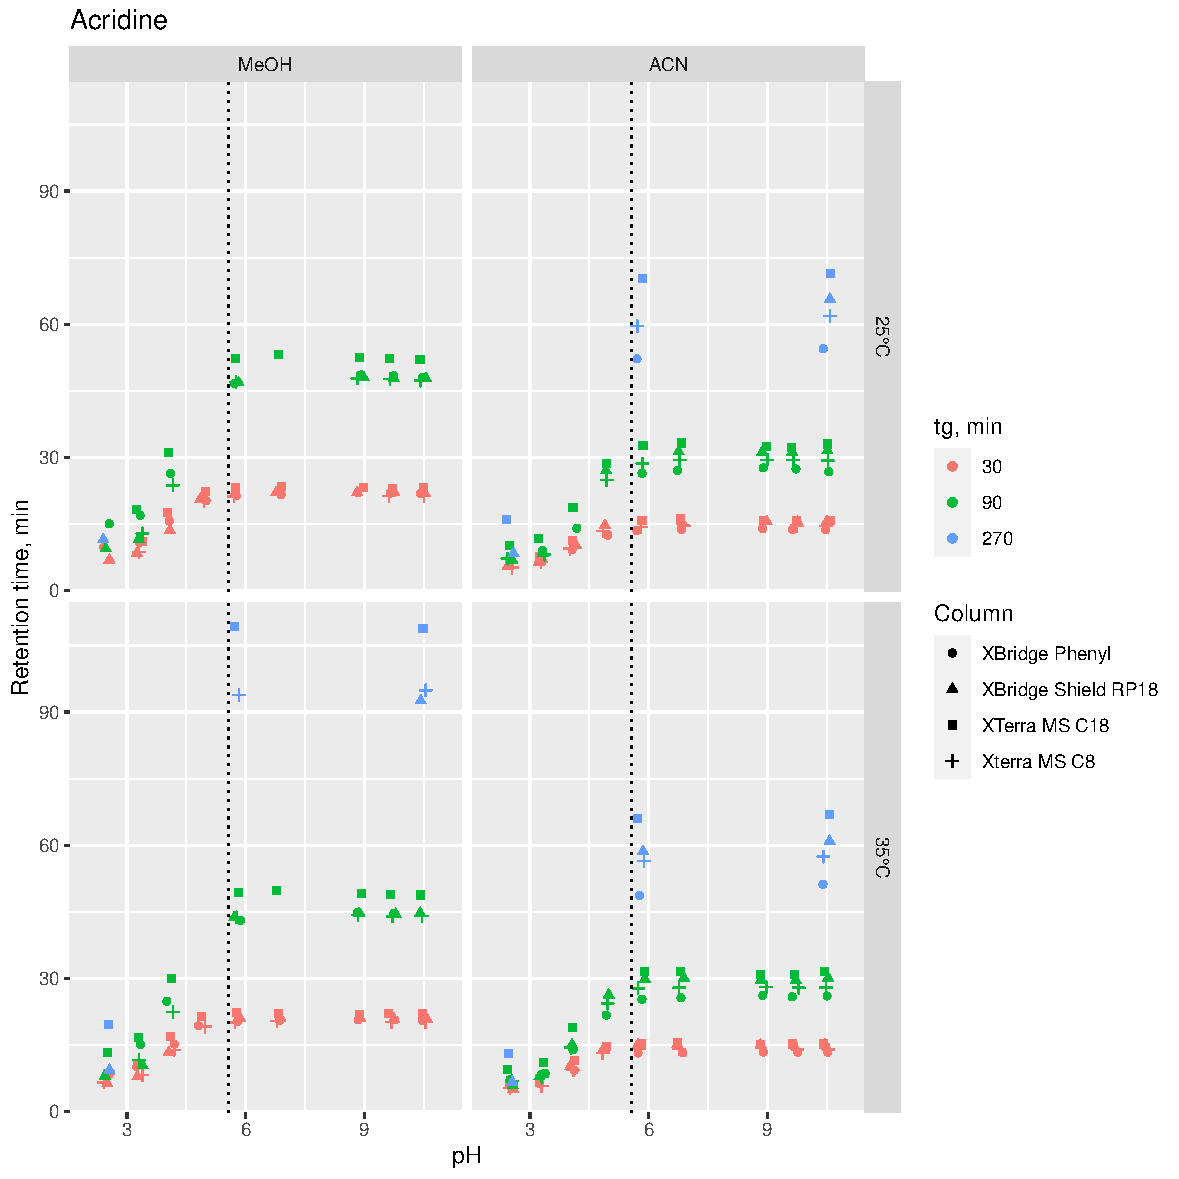
\includegraphics{../figures/rawdata/Acridine.pdf}

\newpage{}

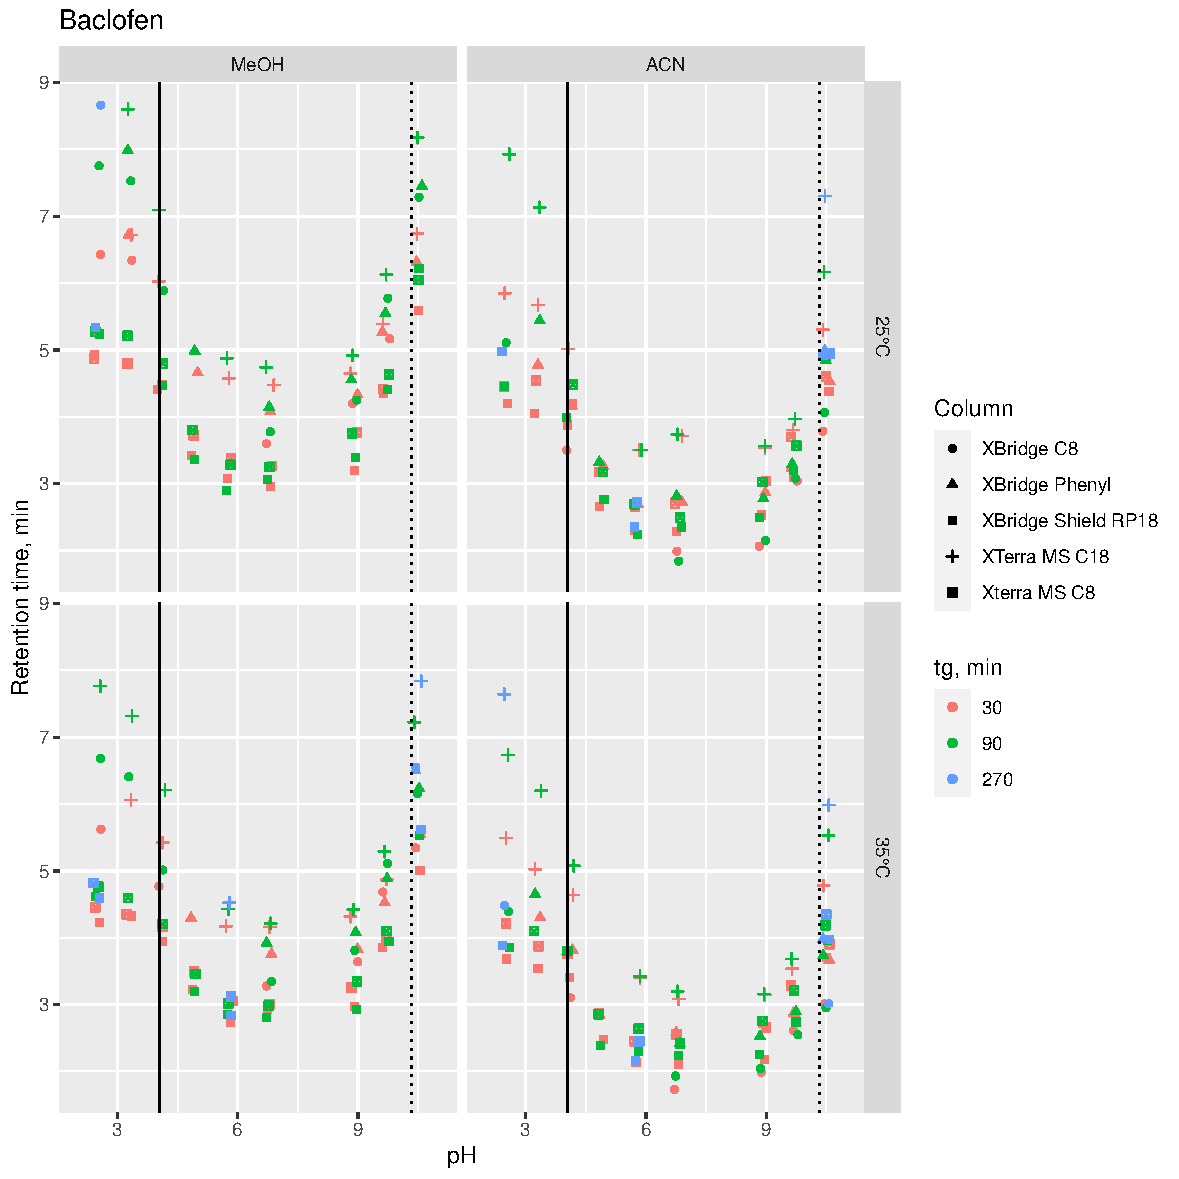
\includegraphics{../figures/rawdata/Baclofen.pdf}

\newpage{}

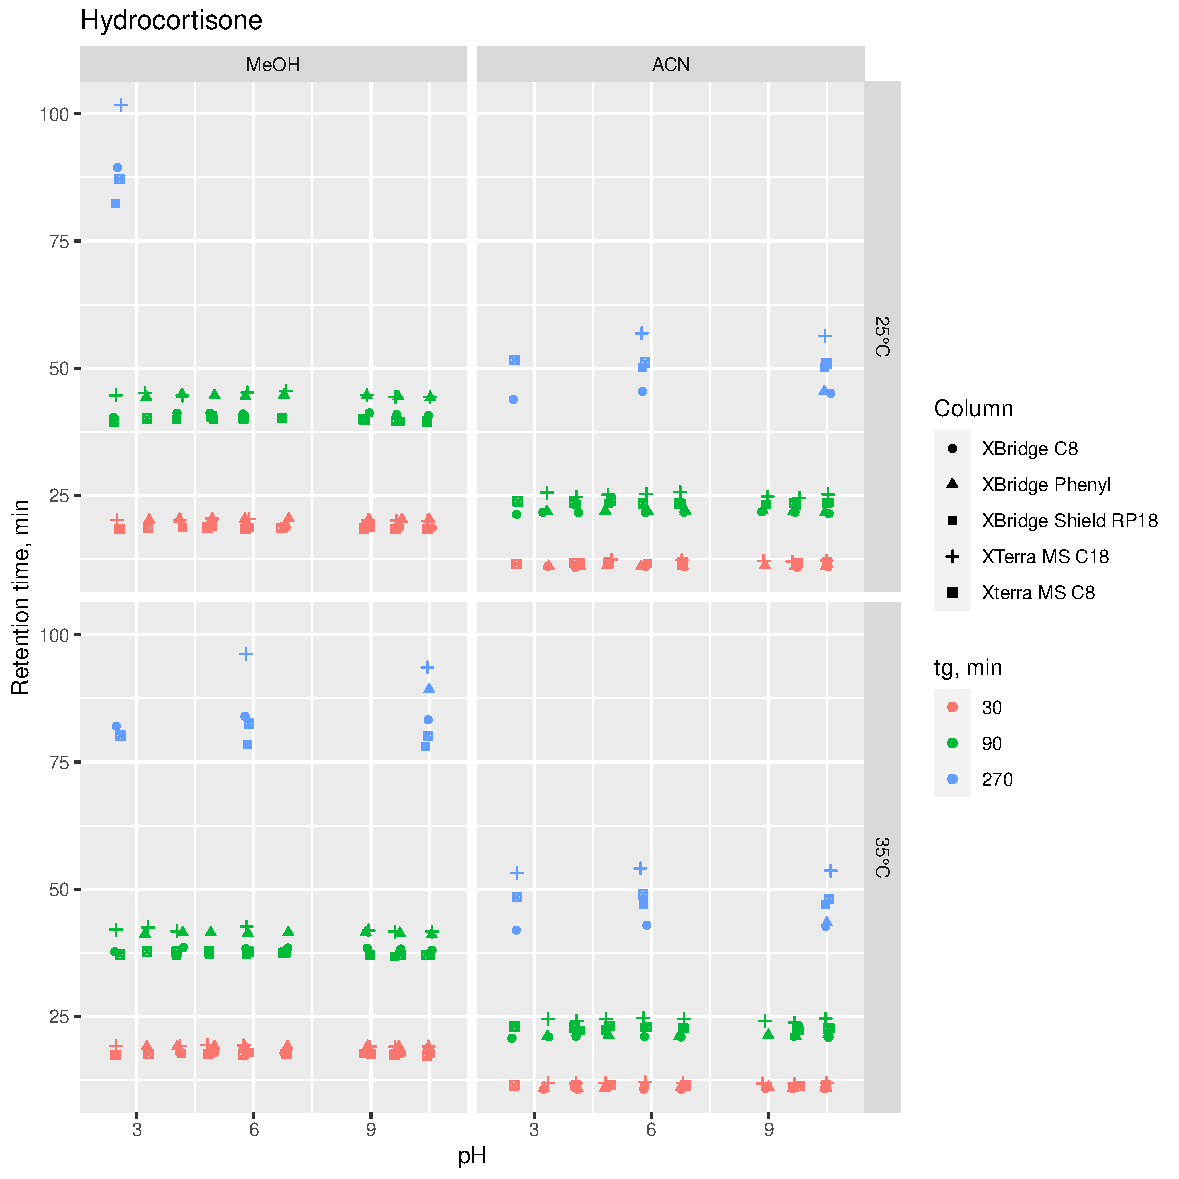
\includegraphics{../figures/rawdata/Hydrocortisone.pdf}

\newpage{}

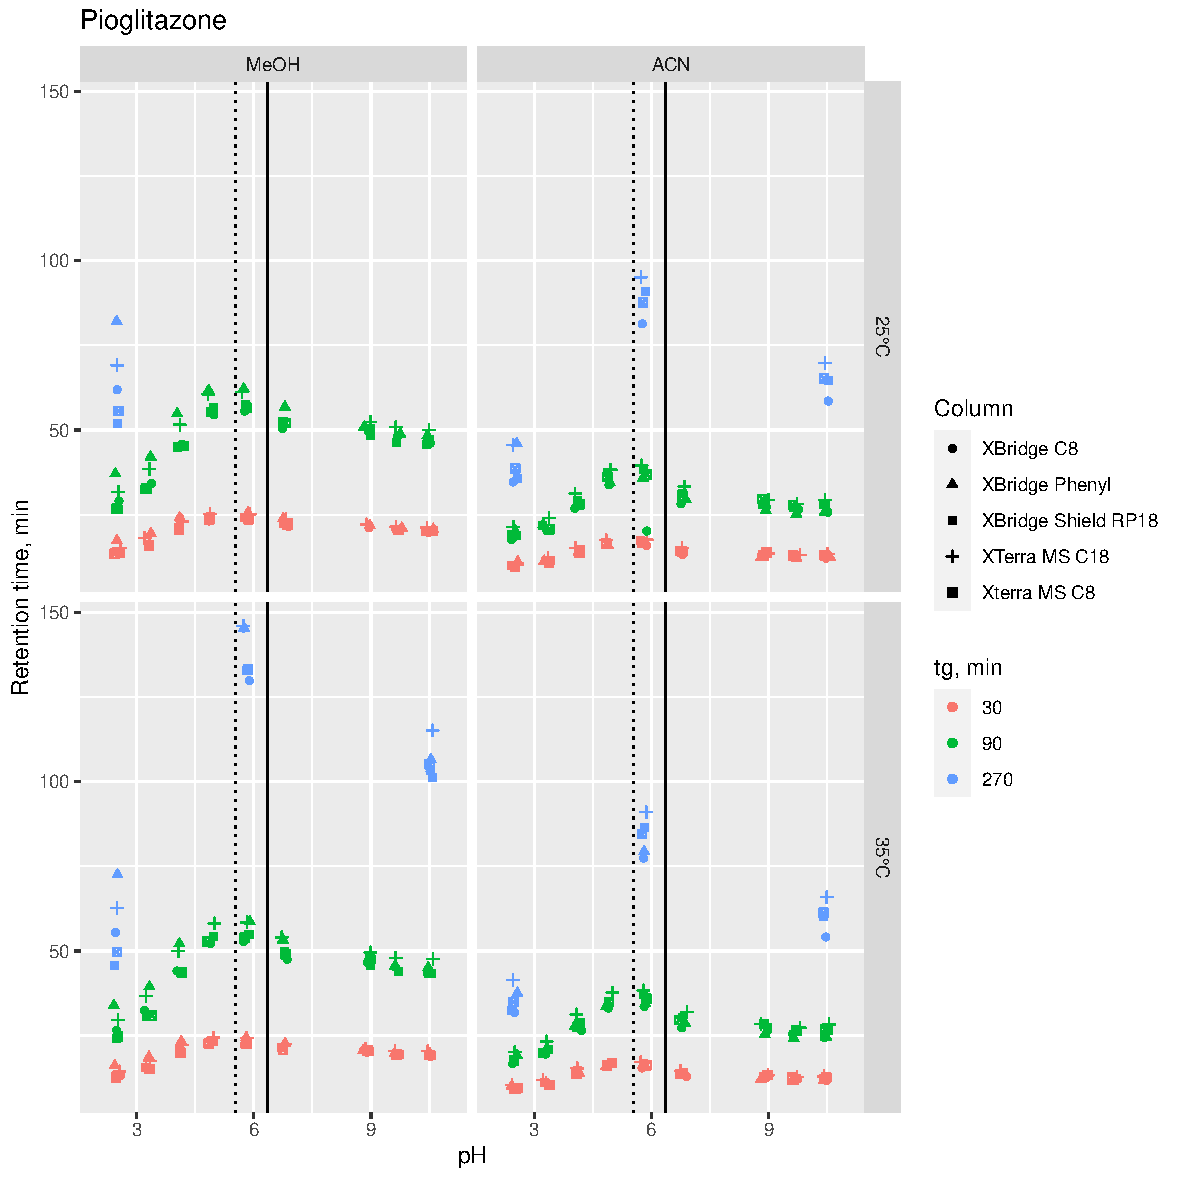
\includegraphics{../figures/rawdata/Pioglitazone.pdf}

\newpage{}

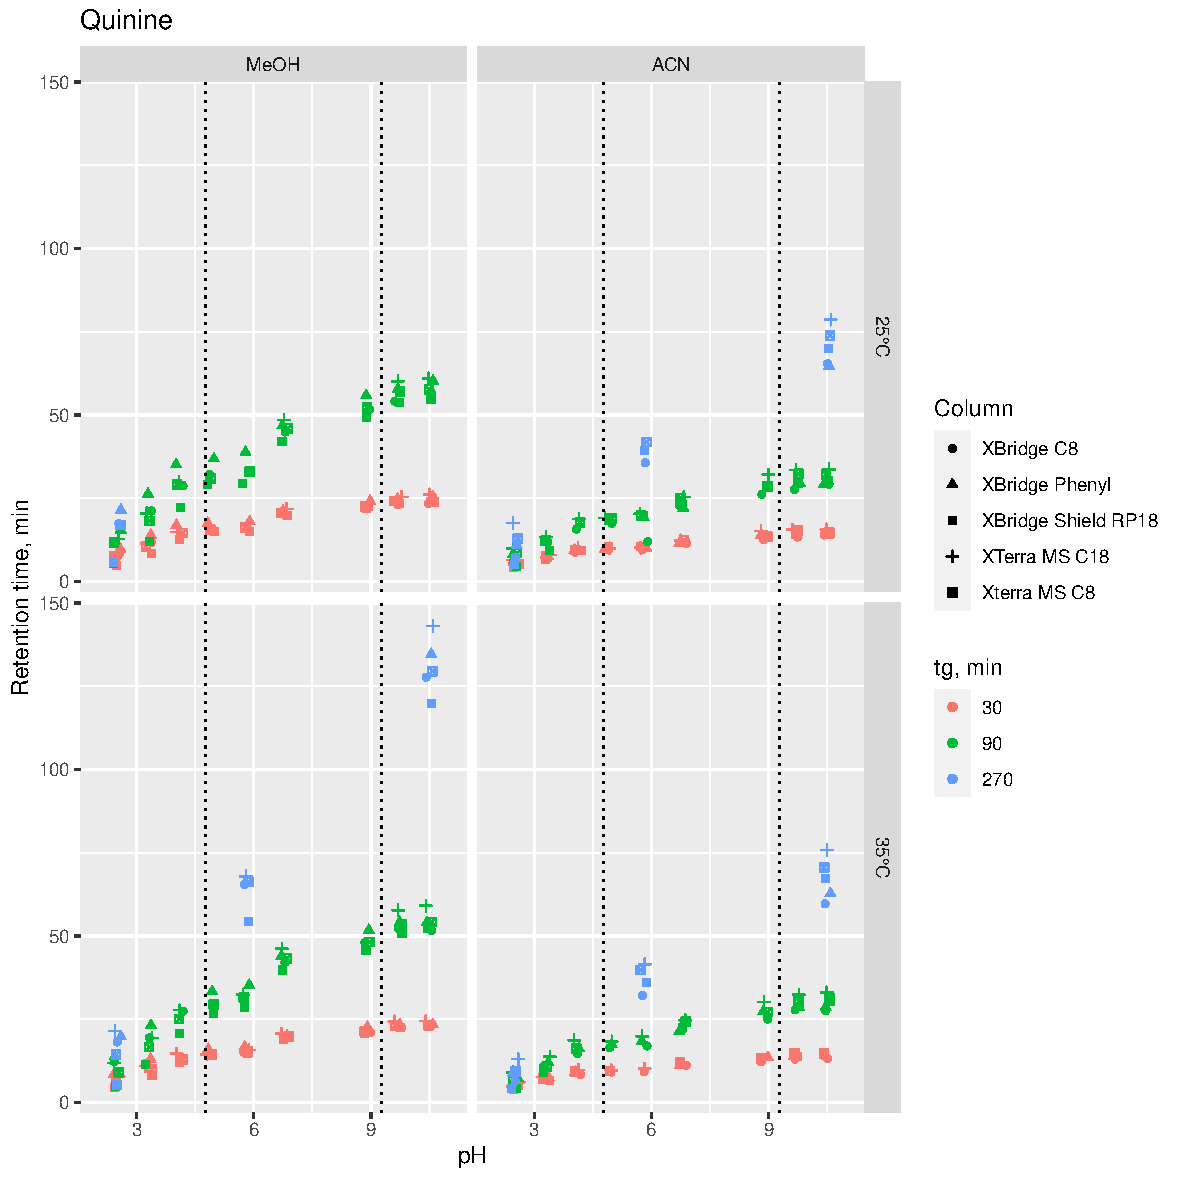
\includegraphics{../figures/rawdata/Quinine.pdf}

\newpage{}

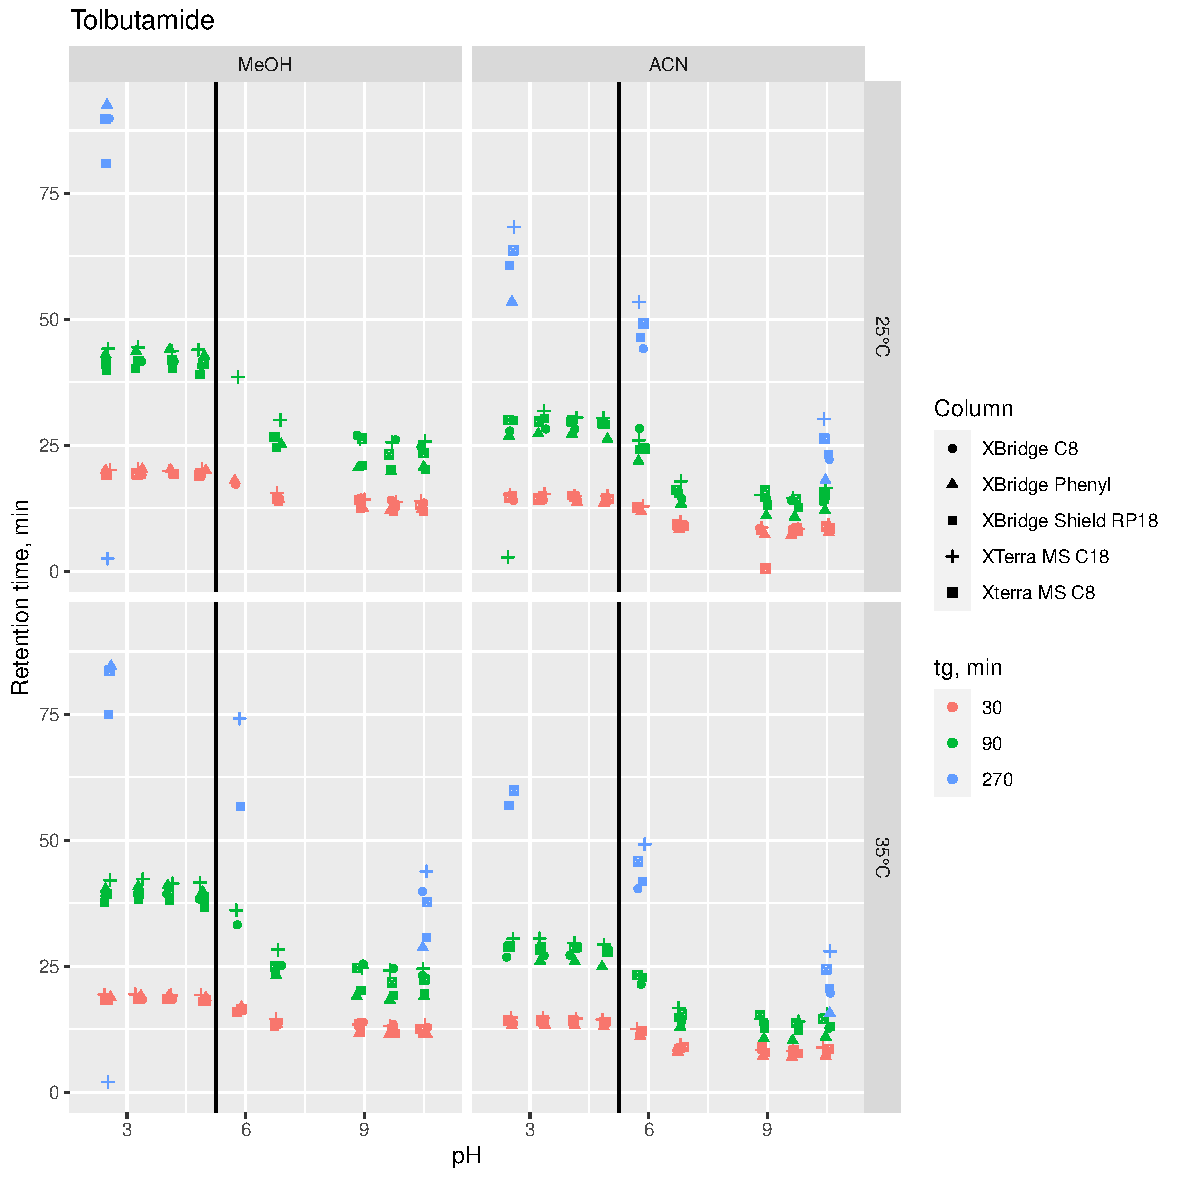
\includegraphics{../figures/rawdata/Tolbutamide.pdf}

\newpage{}

\hypertarget{figure-s2.-summary-of-the-mcmc-simulations-of-the-marginal-posterior-distributions-of-population-level-model-parameters.}{%
\section{Figure S2. Summary of the MCMC simulations of the marginal
posterior distributions of population-level model
parameters.}\label{figure-s2.-summary-of-the-mcmc-simulations-of-the-marginal-posterior-distributions-of-population-level-model-parameters.}}

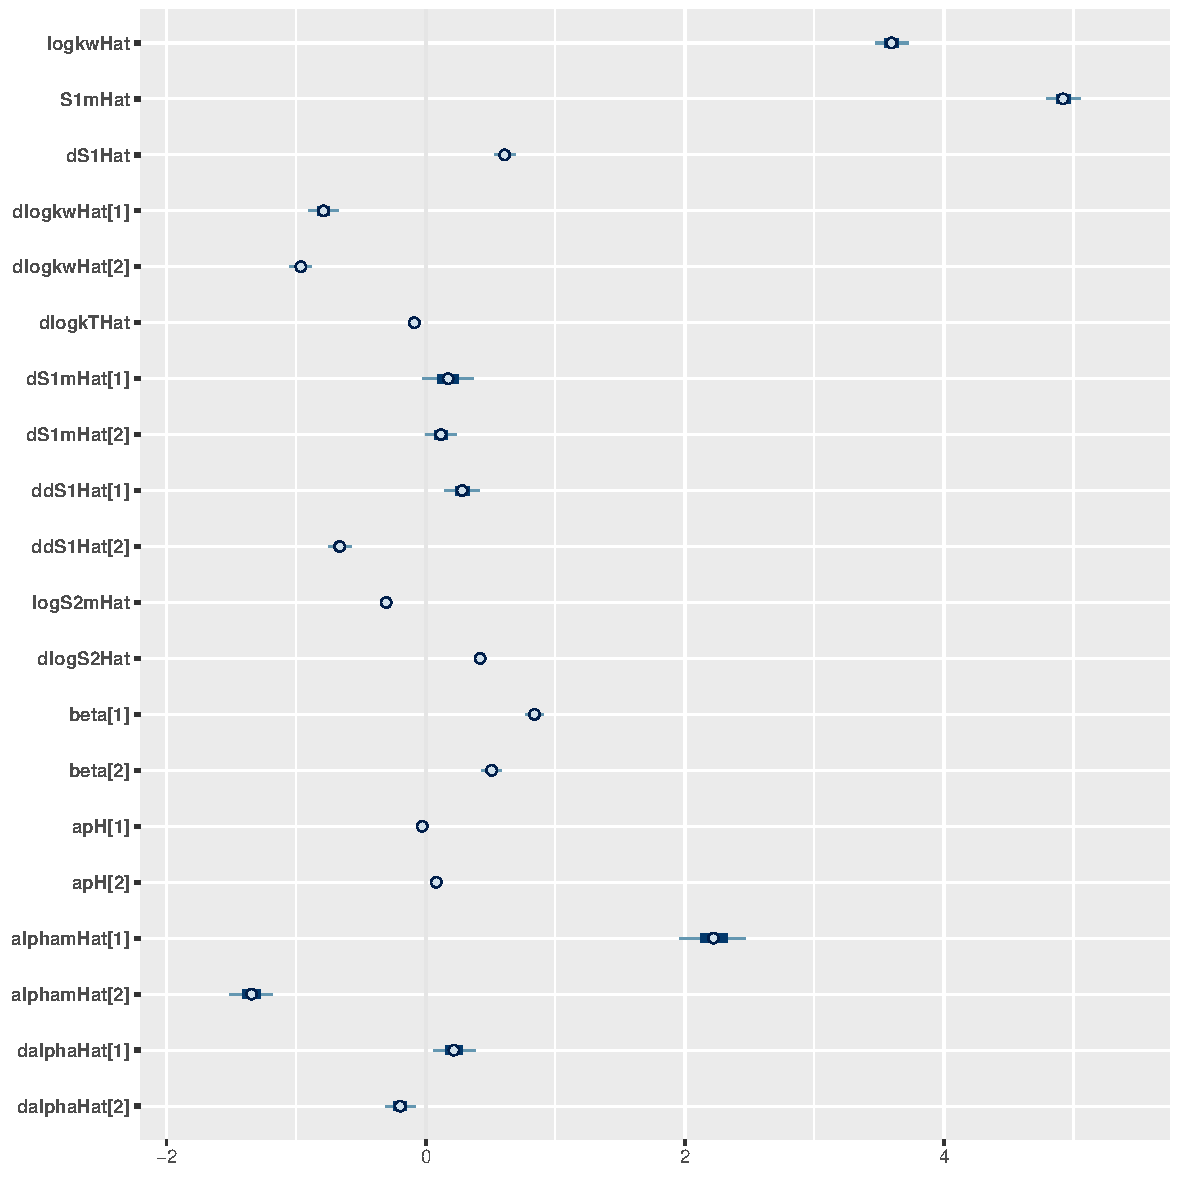
\includegraphics{../figures/param/XBridgeShieldRP18_1.pdf}

\newpage{}

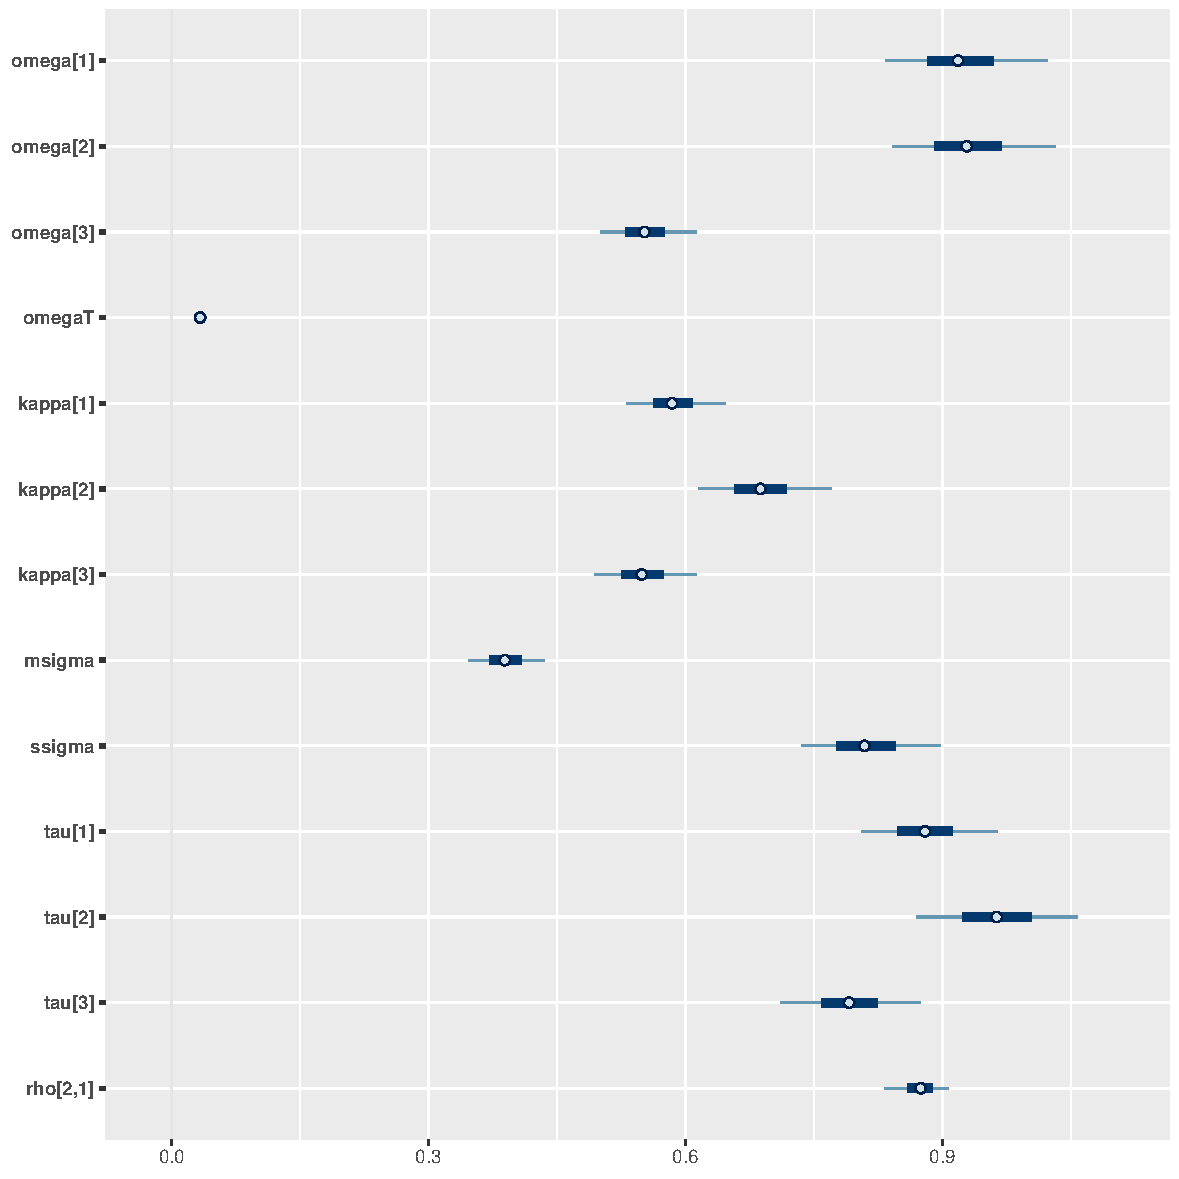
\includegraphics{../figures/param/XBridgeShieldRP18_2.pdf}

\newpage{}

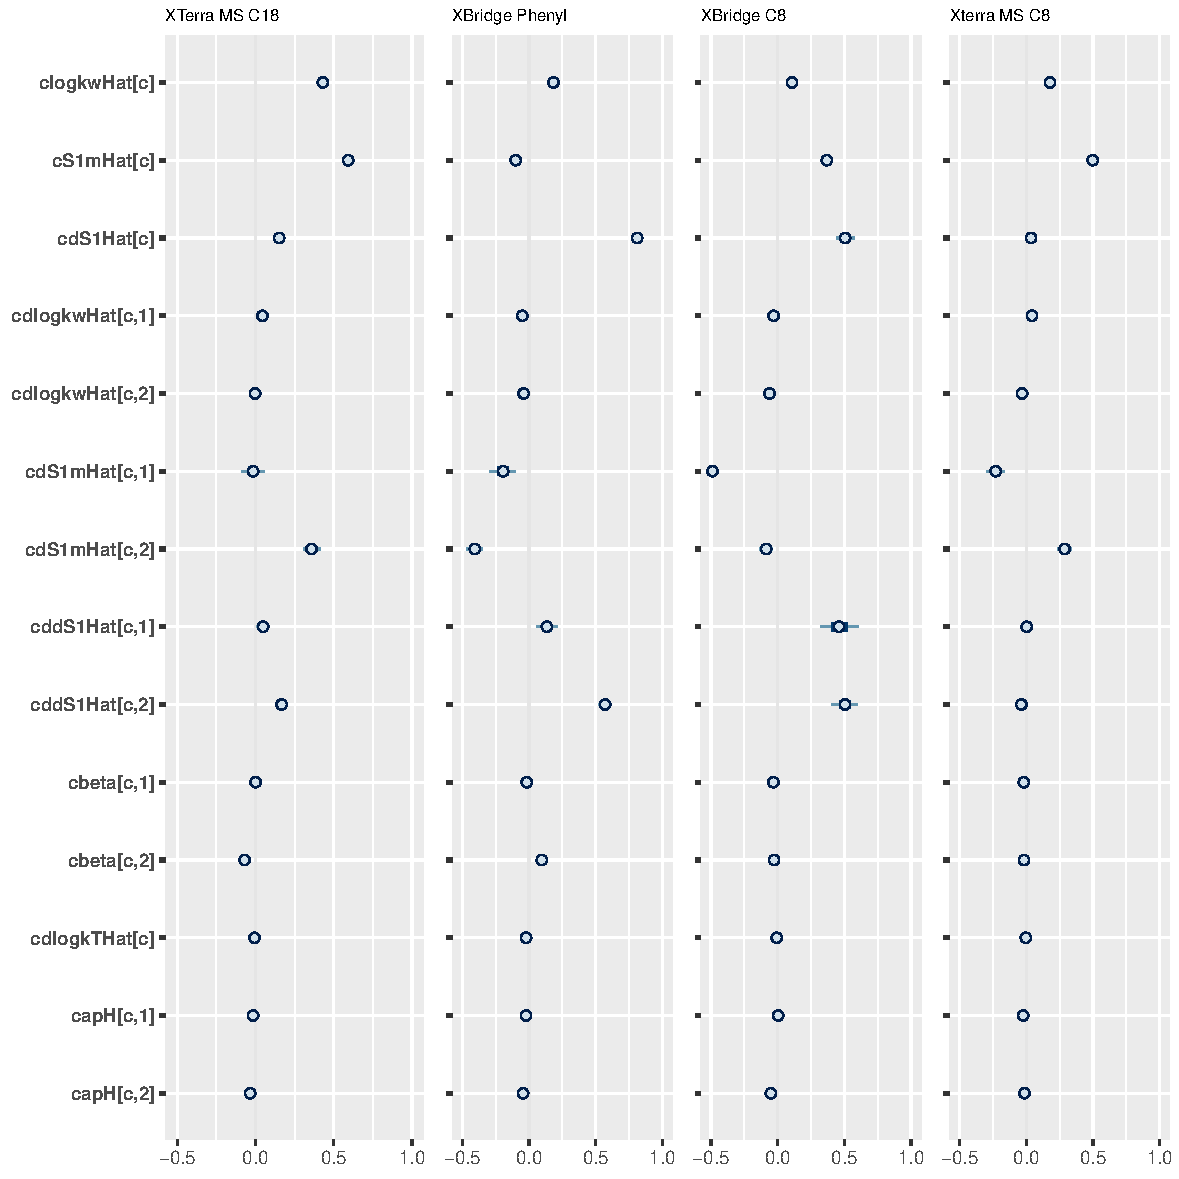
\includegraphics{../figures/param/columneffects1.pdf}

\newpage{}

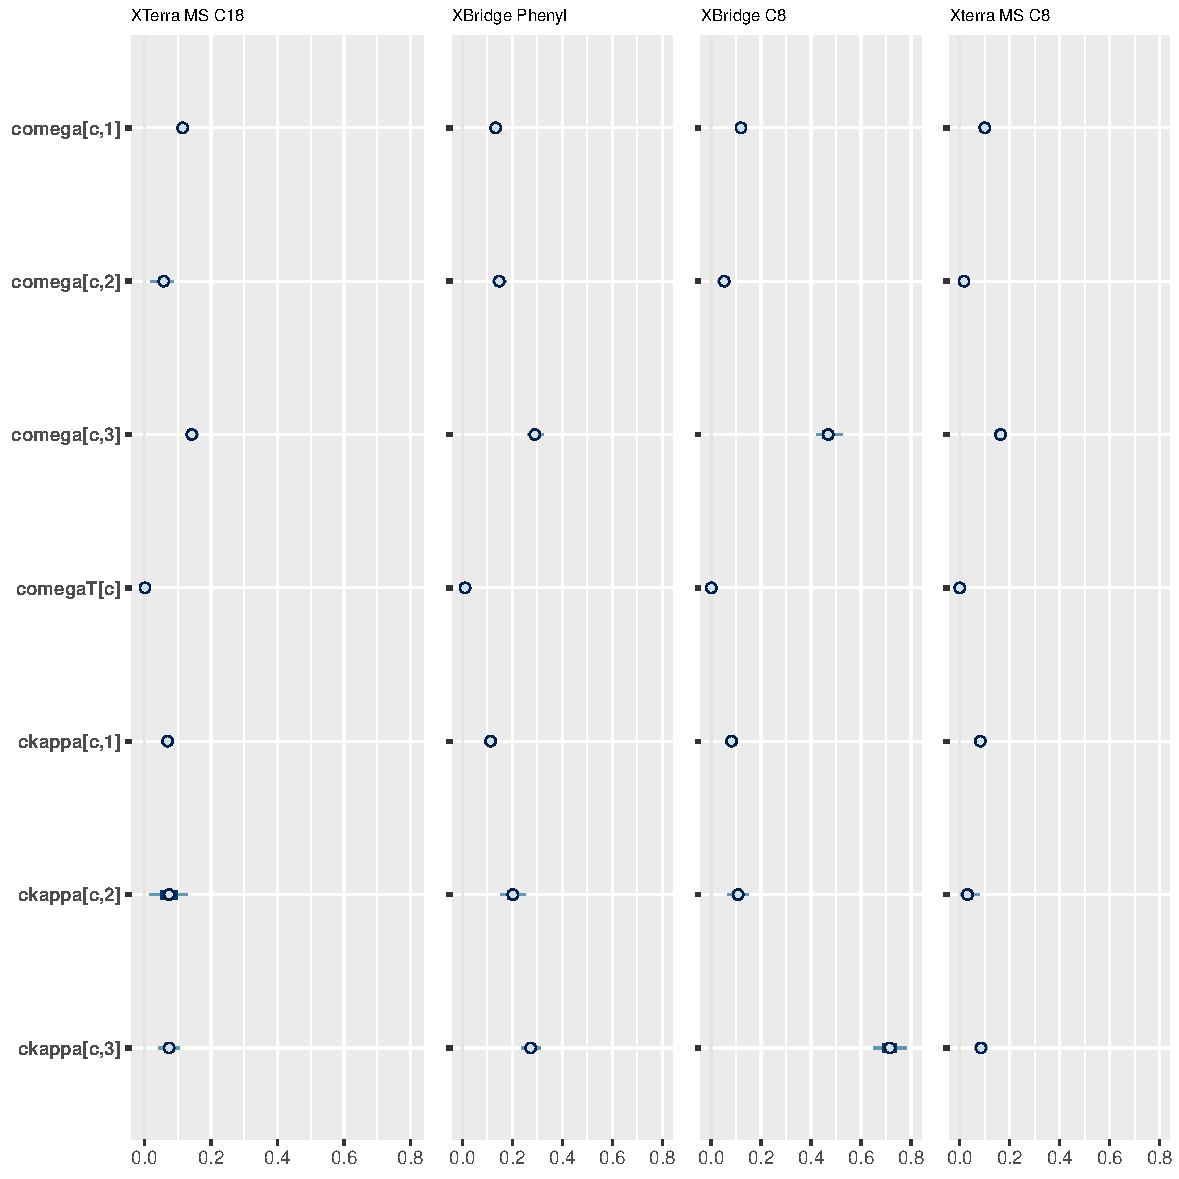
\includegraphics{../figures/param/columneffects2.pdf}

\newpage{}

\hypertarget{figure-s3.-goodness-of-fit-plots.}{%
\section{Figure S3. Goodness of fit
plots.}\label{figure-s3.-goodness-of-fit-plots.}}

Individual residuals:

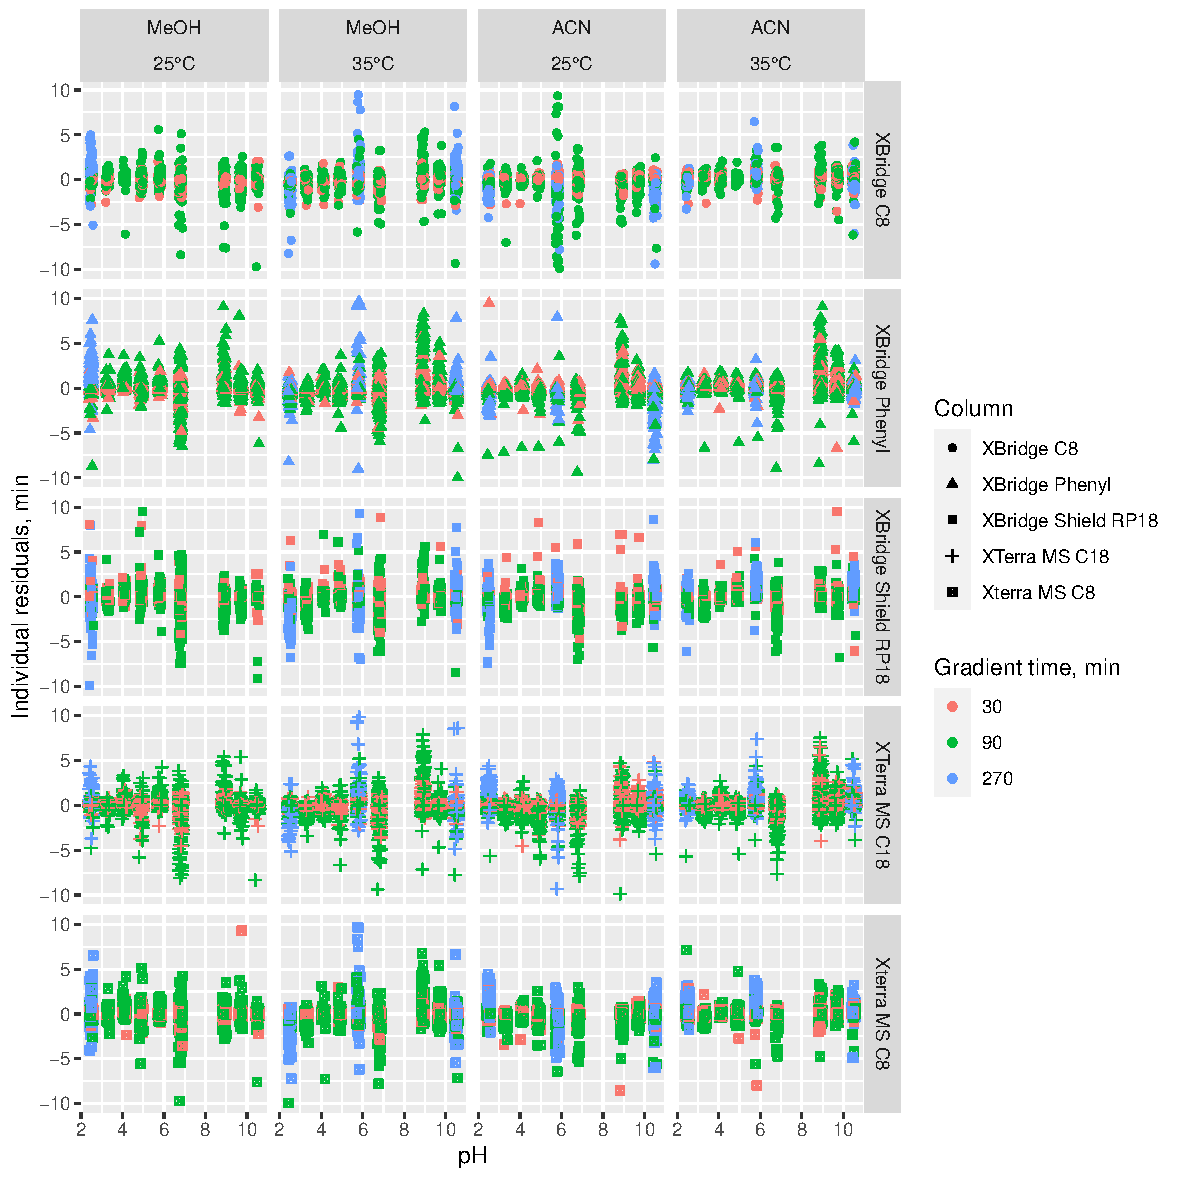
\includegraphics{../figures/concordanceplots/individualresiduals.pdf}

\newpage{}

Population residuals:

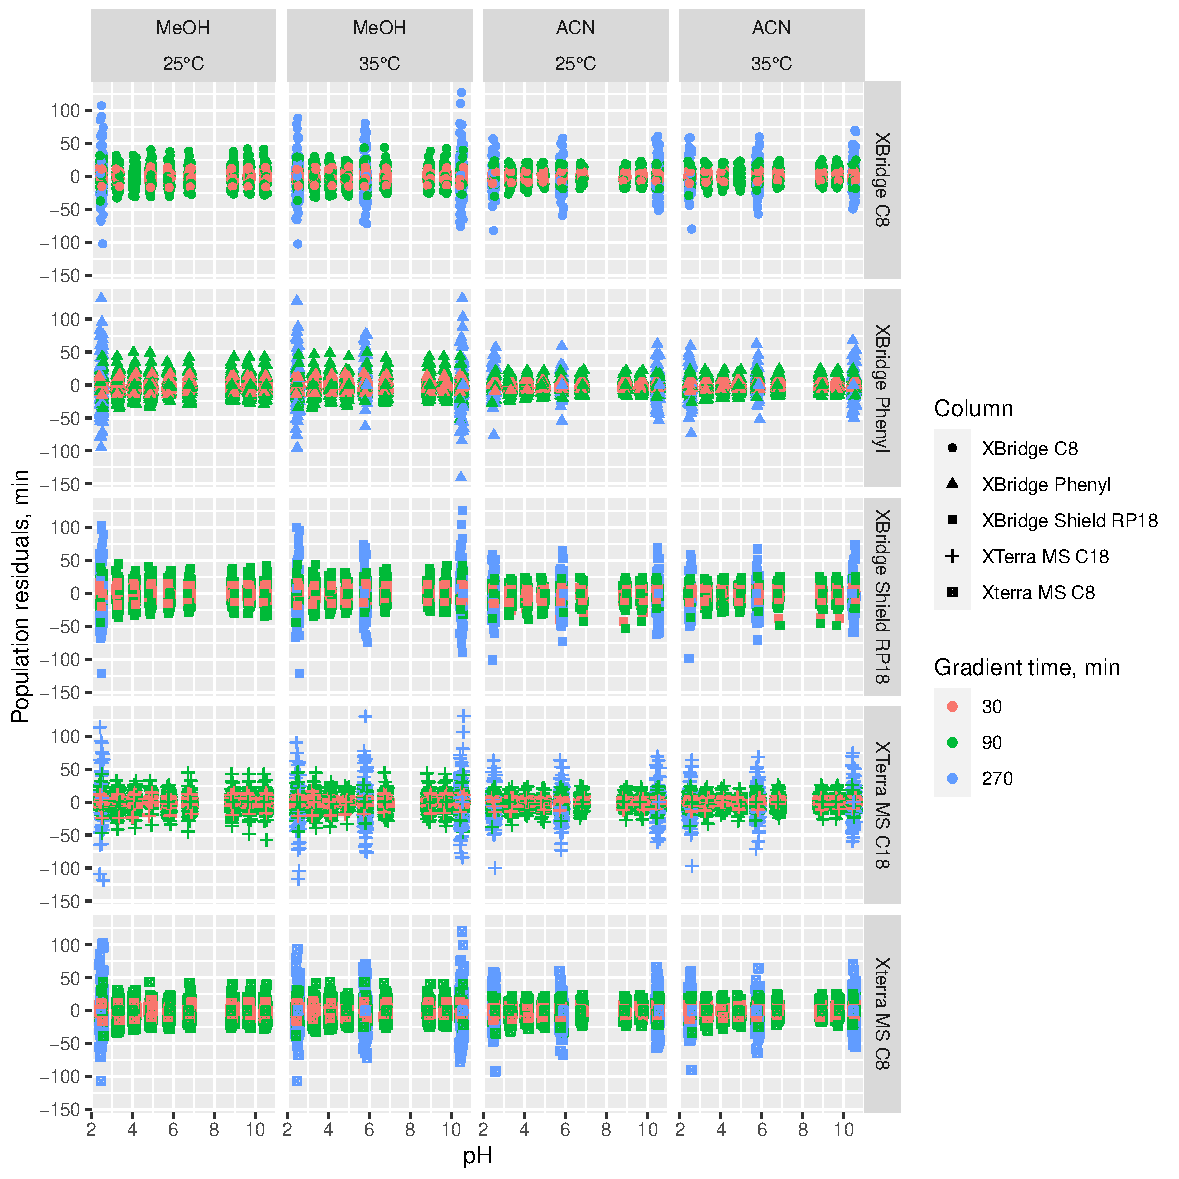
\includegraphics{../figures/concordanceplots/populationresiduals.pdf}

\newpage{}

The observed vs.~the mean individual-predicted retention times (i.e., a
posteriori mean of a predictive distribution conditioned on the observed
data from the same analyte).
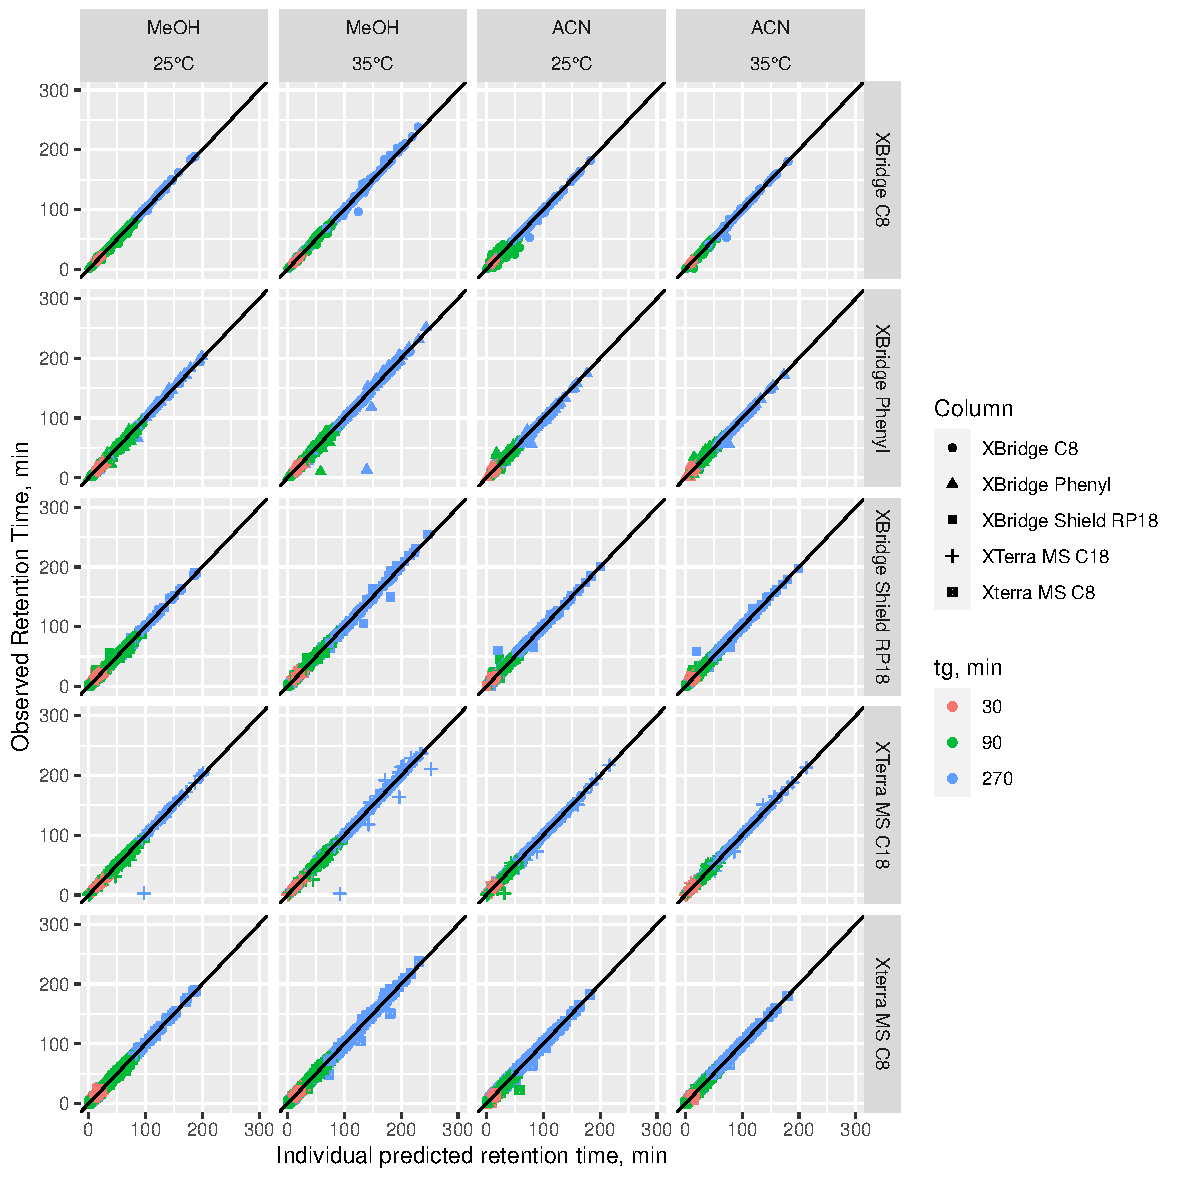
\includegraphics{../figures/concordanceplots/individual.pdf}

\newpage{}

The observed vs.~the mean population-predicted retention times (i.e., a
posteriori means of predictive distributions corresponding to the future
observations of a new analyte)
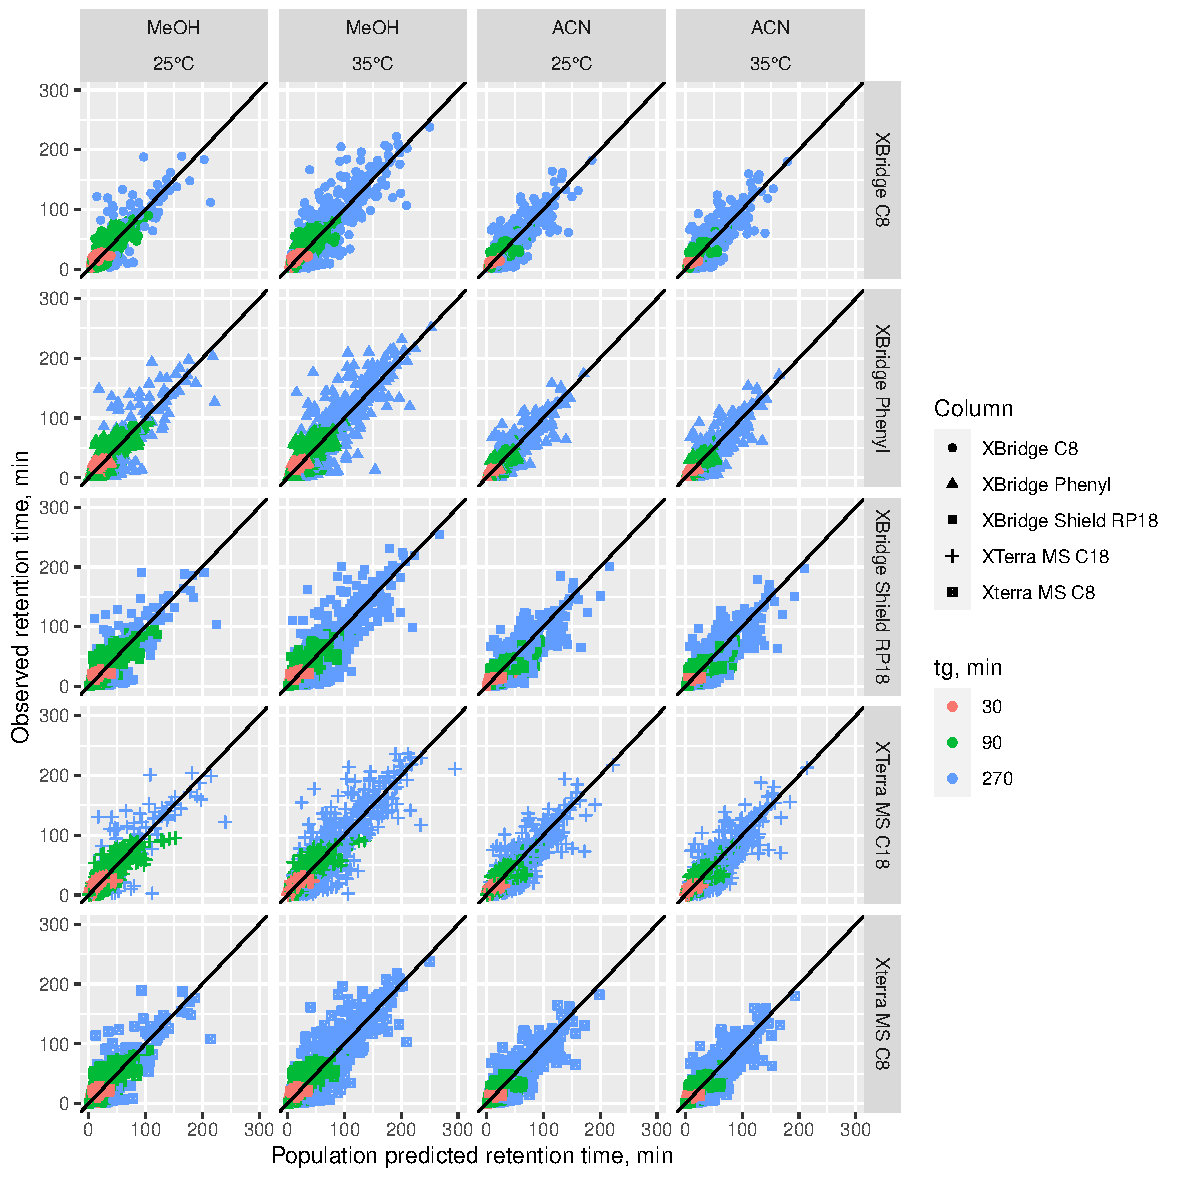
\includegraphics{../figures/concordanceplots/population.pdf}

\newpage{}

\hypertarget{figure-s4.-individual-gradient-predictions.}{%
\section{Figure S4. Individual gradient
predictions.}\label{figure-s4.-individual-gradient-predictions.}}

Predictions represented as posterior median (line) and 5th-95th
percentiles (areas) for a 6 exemplary analytes. Predictions
corresponding to future observations given the population-level
parameters and all the retention data measured for a particular analyte.

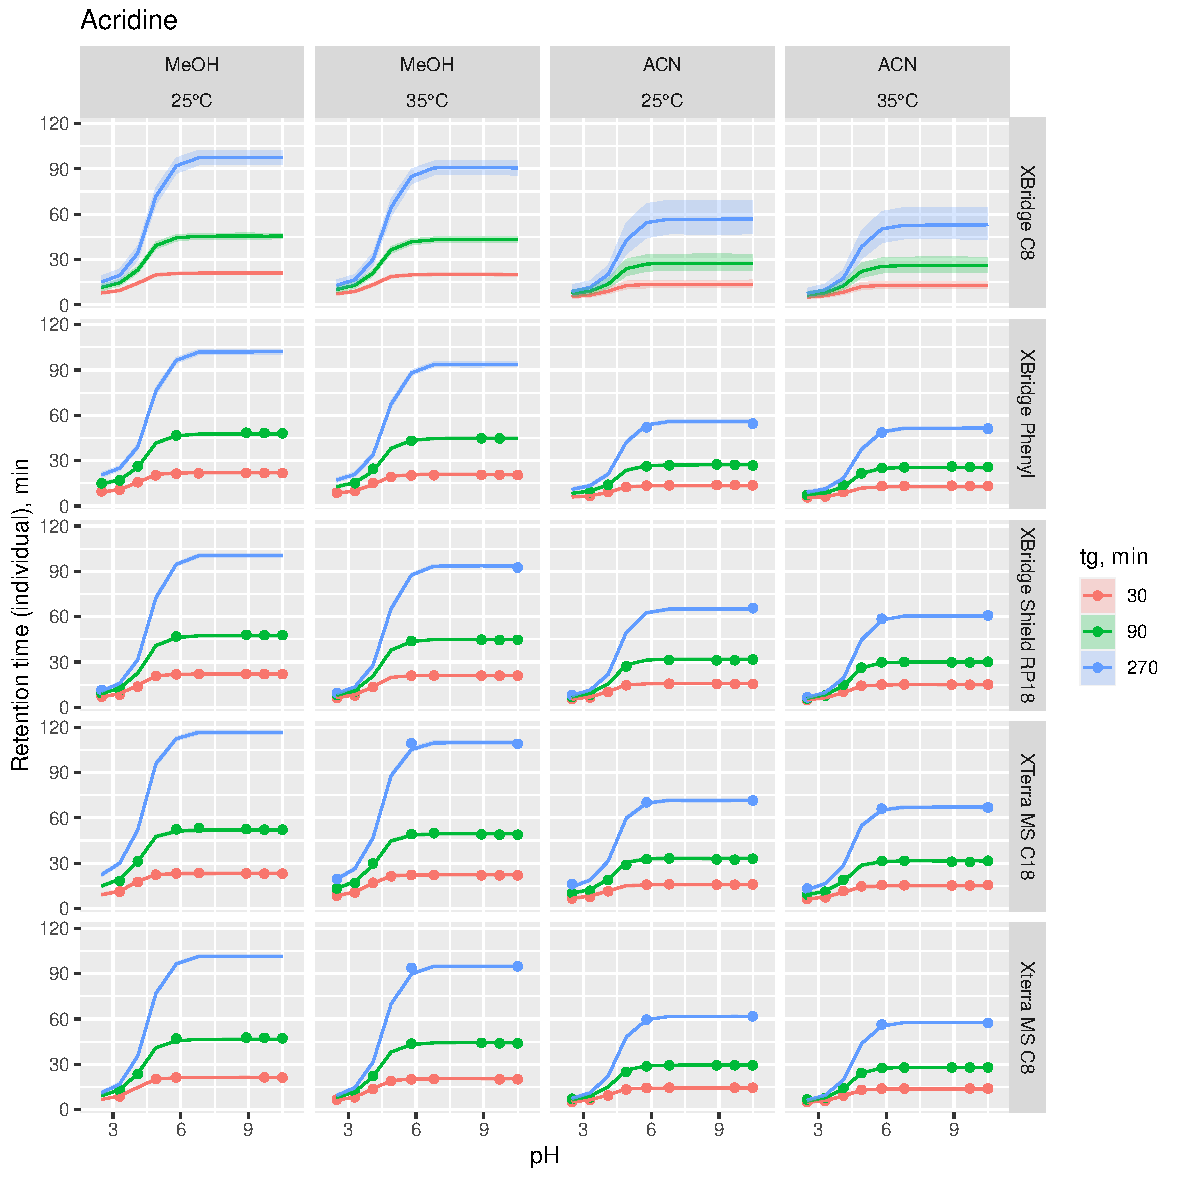
\includegraphics{../figures/concordanceplots/Acridine.individual.pdf}

\newpage{}

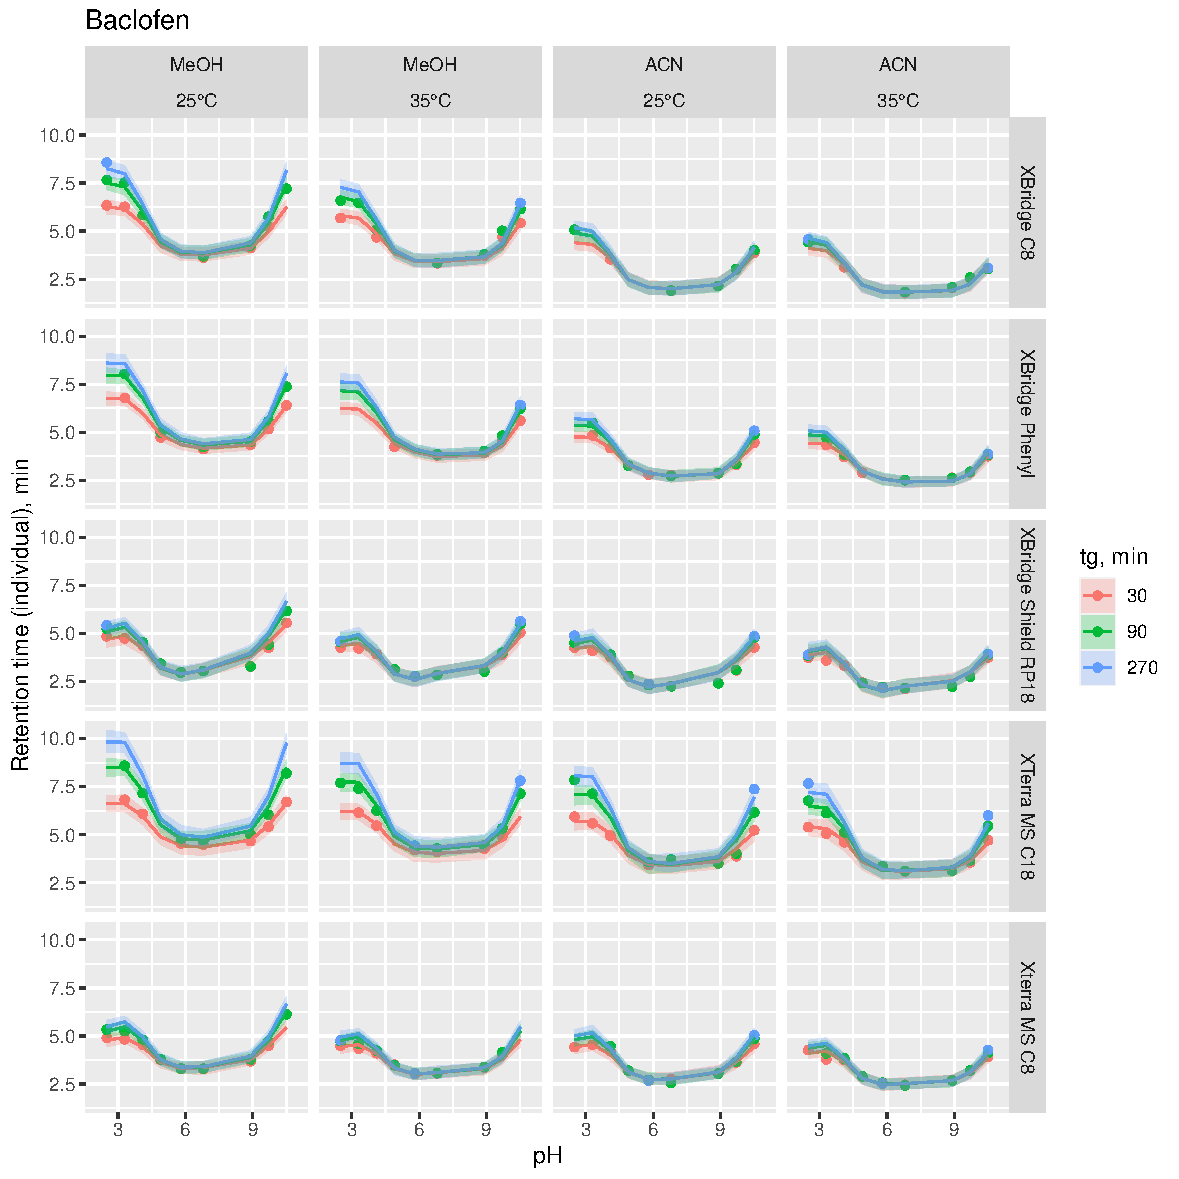
\includegraphics{../figures/concordanceplots/Baclofen.individual.pdf}

\newpage{}

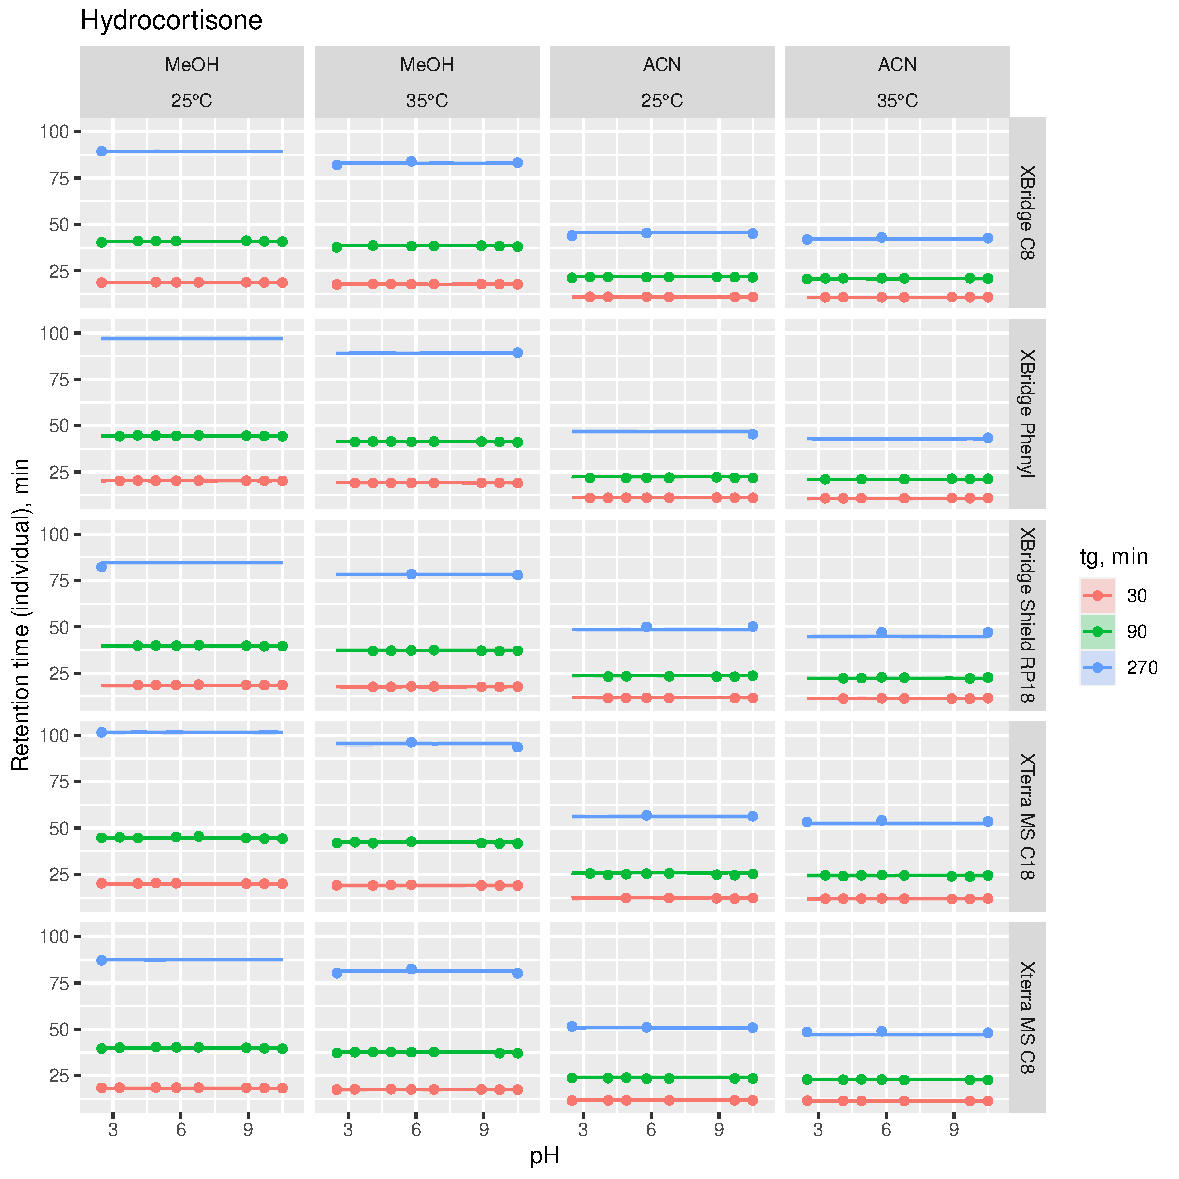
\includegraphics{../figures/concordanceplots/Hydrocortisone.individual.pdf}

\newpage{}

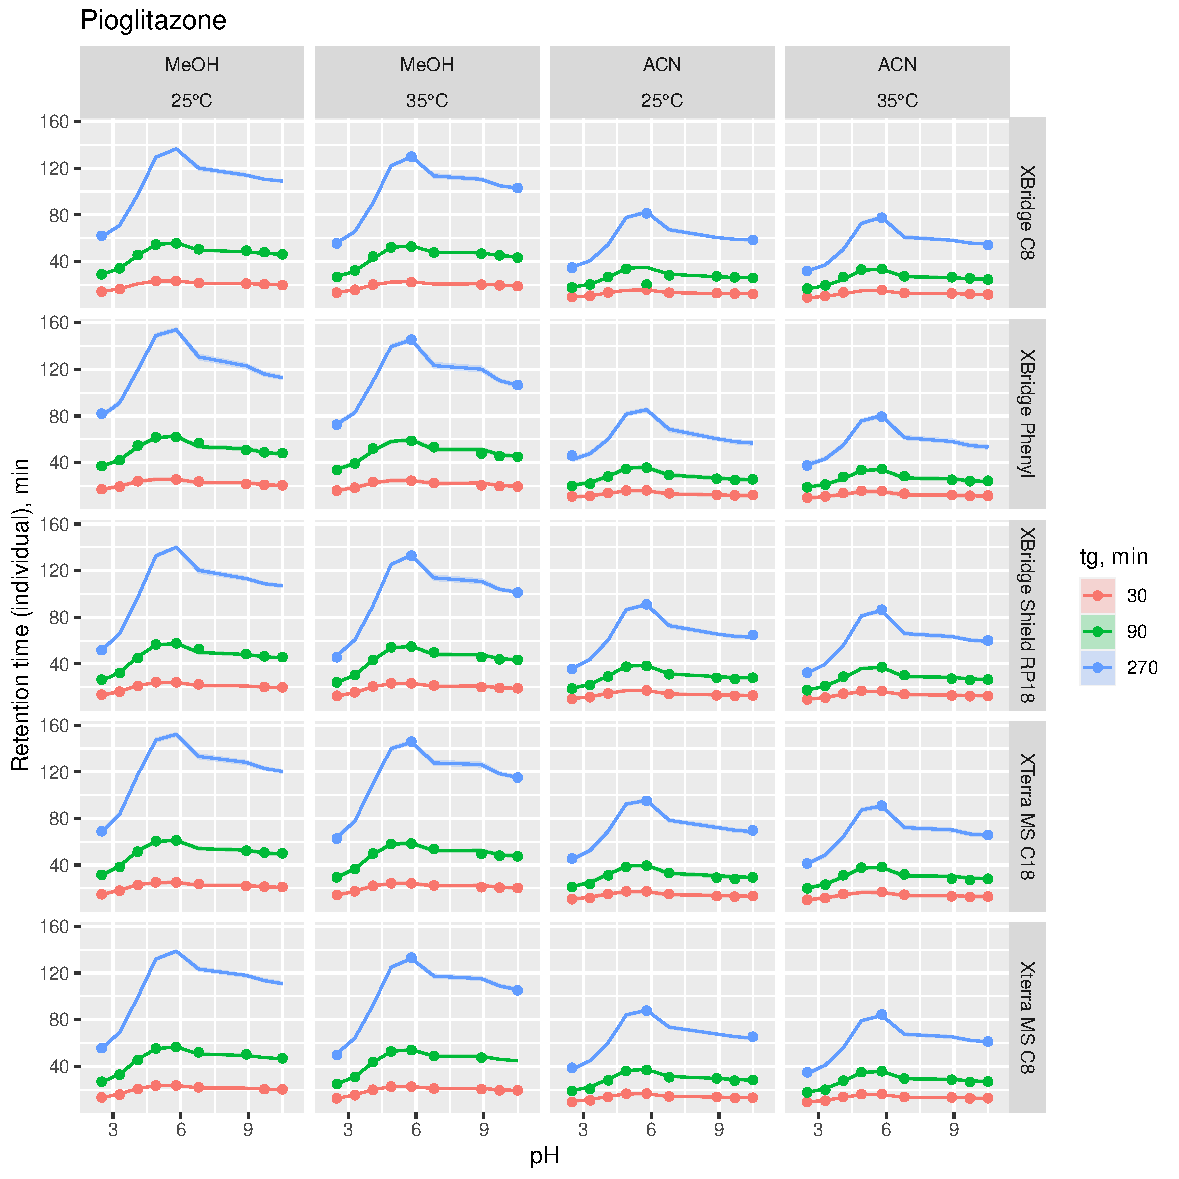
\includegraphics{../figures/concordanceplots/Pioglitazone.individual.pdf}

\newpage{}

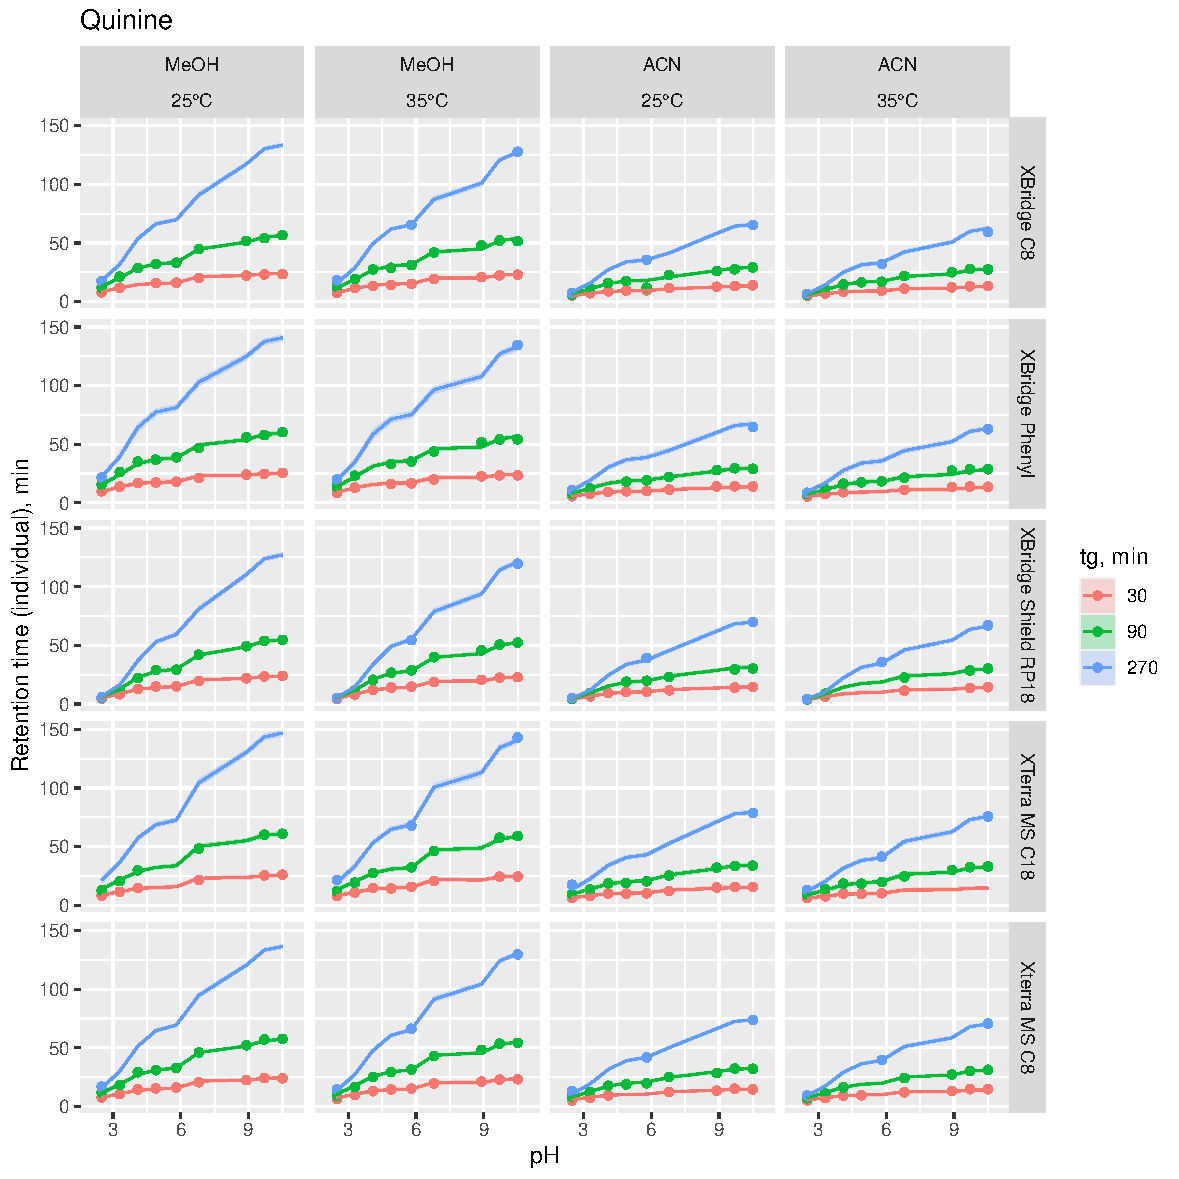
\includegraphics{../figures/concordanceplots/Quinine.individual.pdf}

\newpage{}

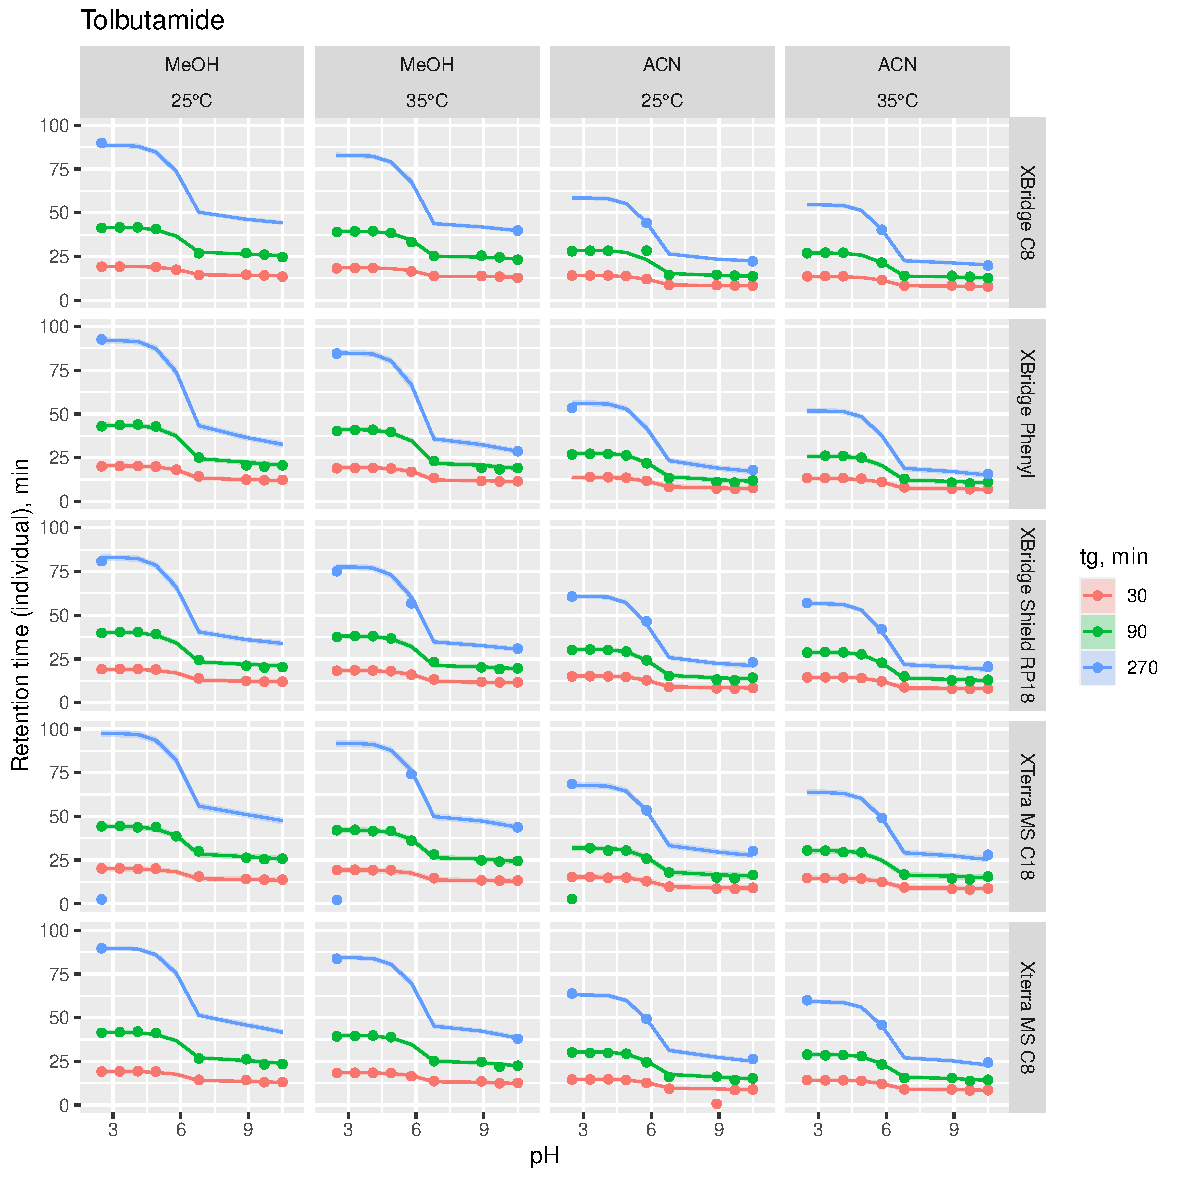
\includegraphics{../figures/concordanceplots/Tolbutamide.individual.pdf}

\newpage{}

\hypertarget{figure-s5.-population-gradient-predictions.}{%
\section{Figure S5. Population gradient
predictions.}\label{figure-s5.-population-gradient-predictions.}}

Predictions represented as posterior median (line) and 5th-95th
percentiles (areas) for a 6 exemplary analytes. Predictions
corresponding to future observations given only population-level
parameters and predictors (logP and pKa).

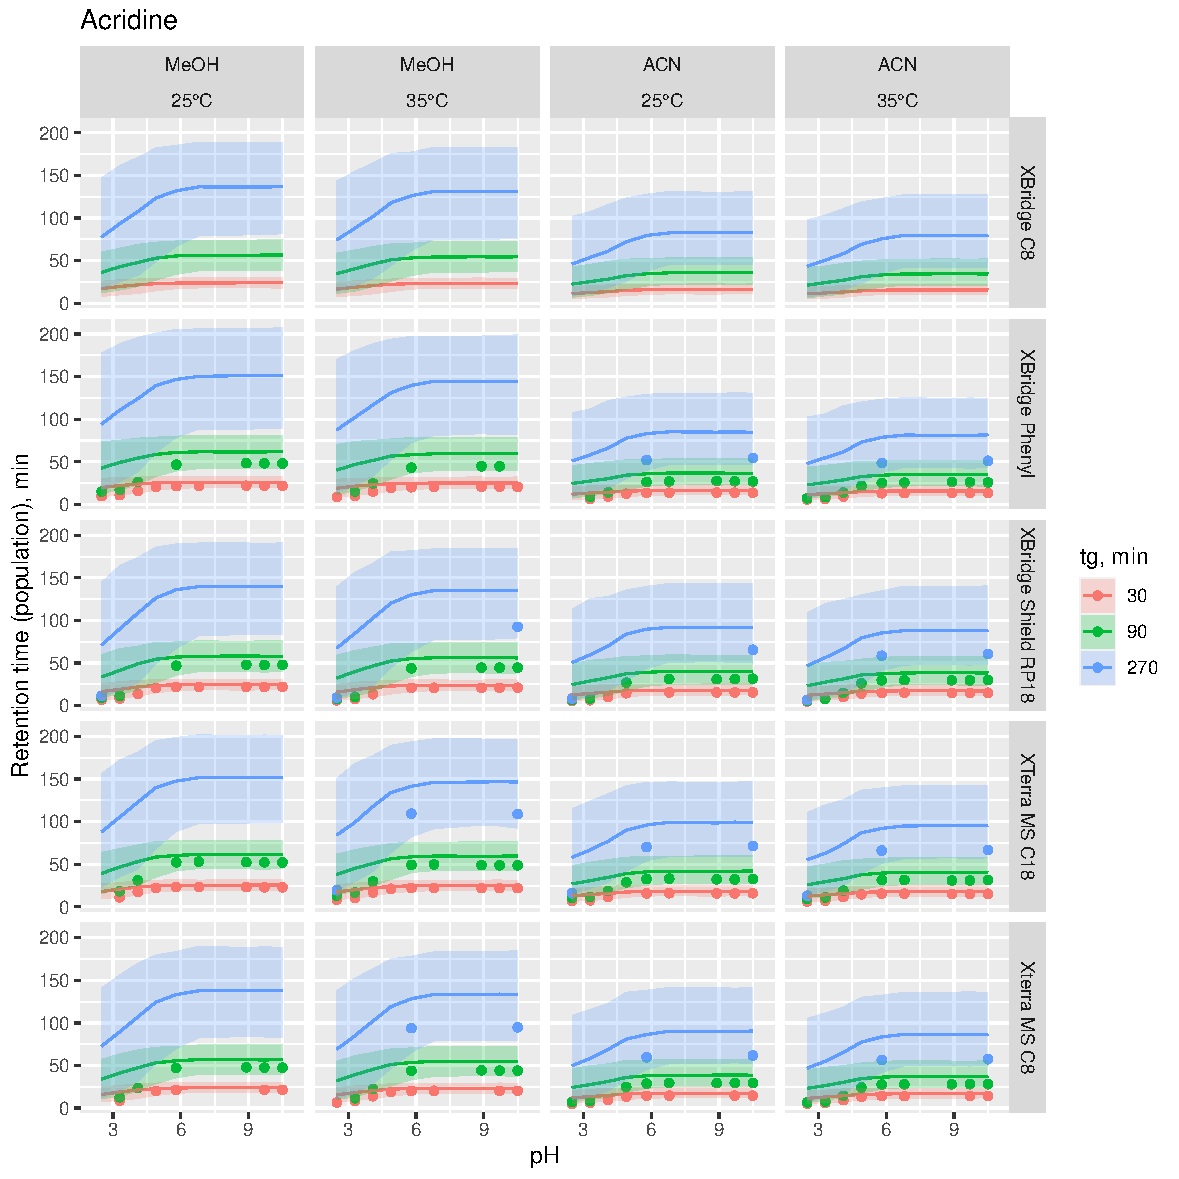
\includegraphics{../figures/concordanceplots/Acridine.population.pdf}

\newpage{}

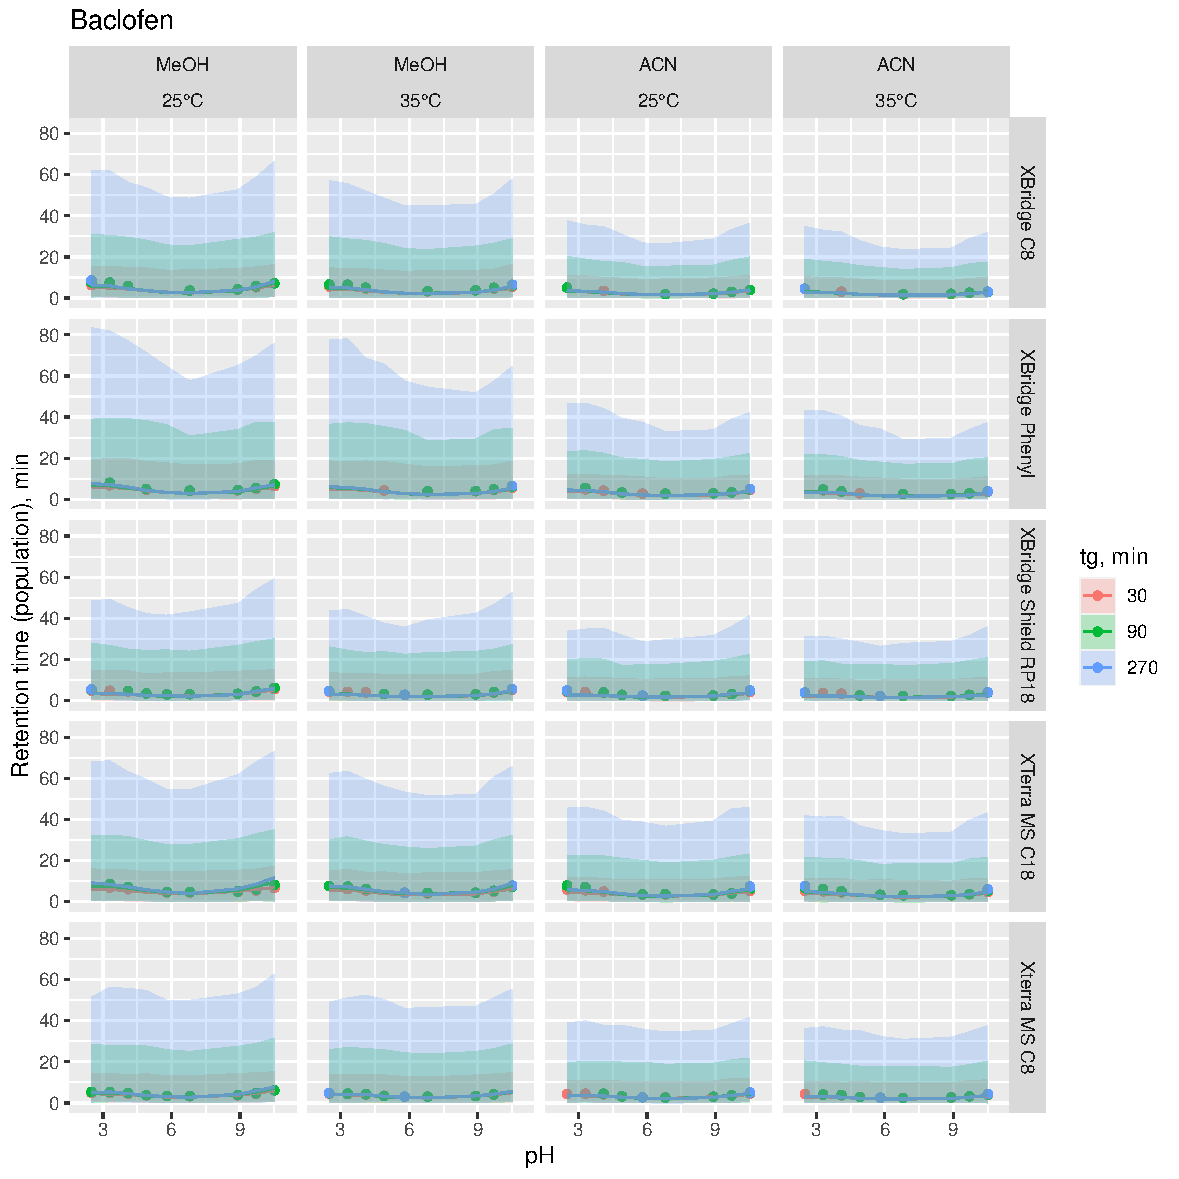
\includegraphics{../figures/concordanceplots/Baclofen.population.pdf}

\newpage{}

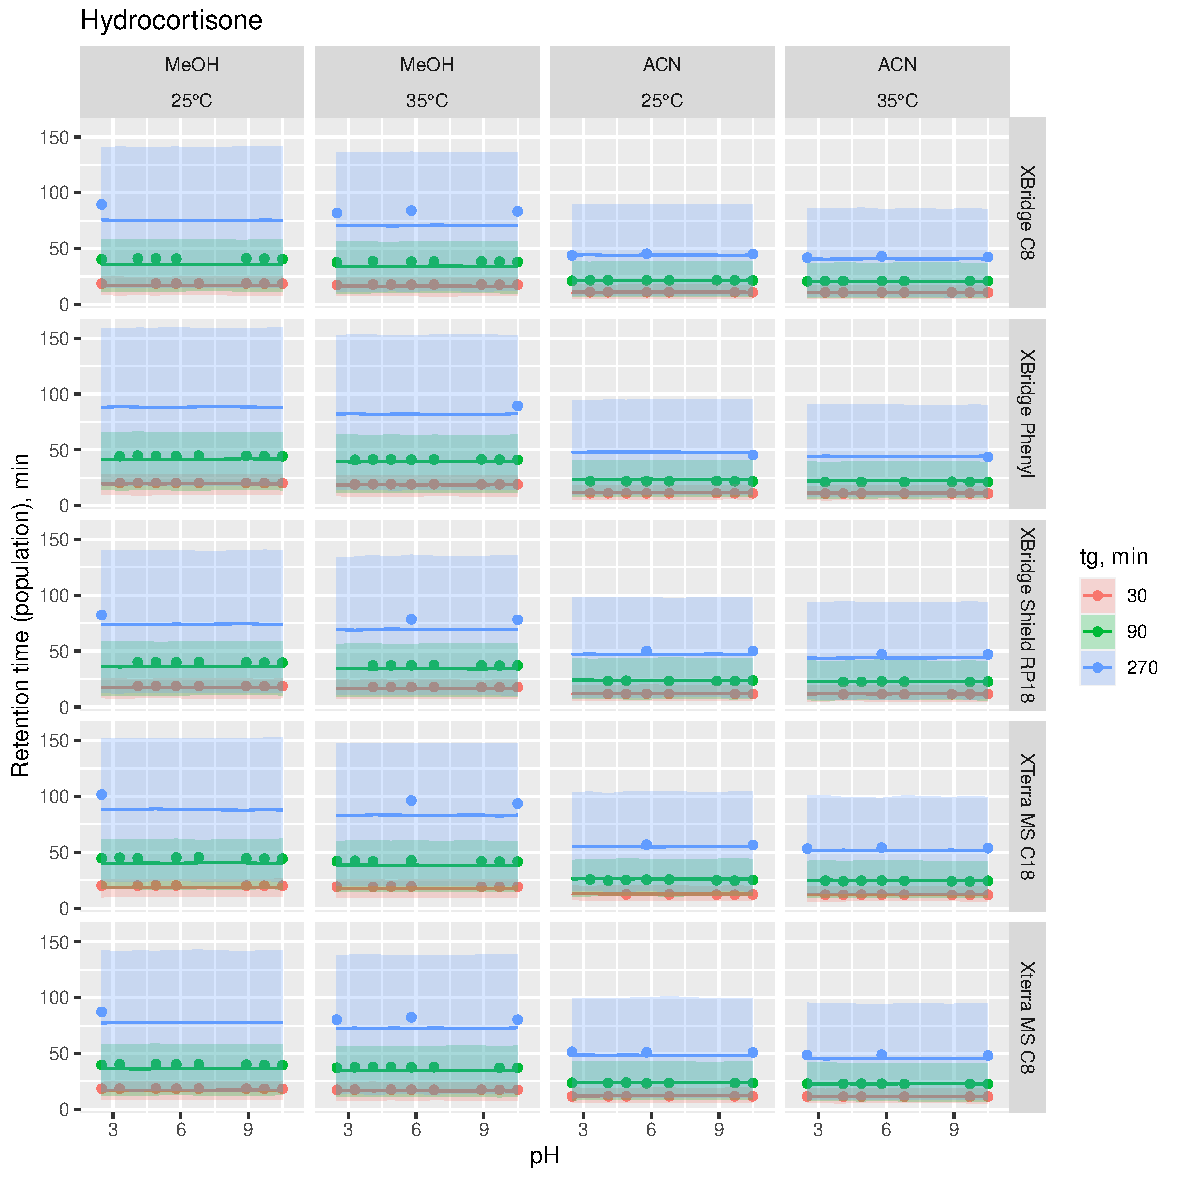
\includegraphics{../figures/concordanceplots/Hydrocortisone.population.pdf}

\newpage{}

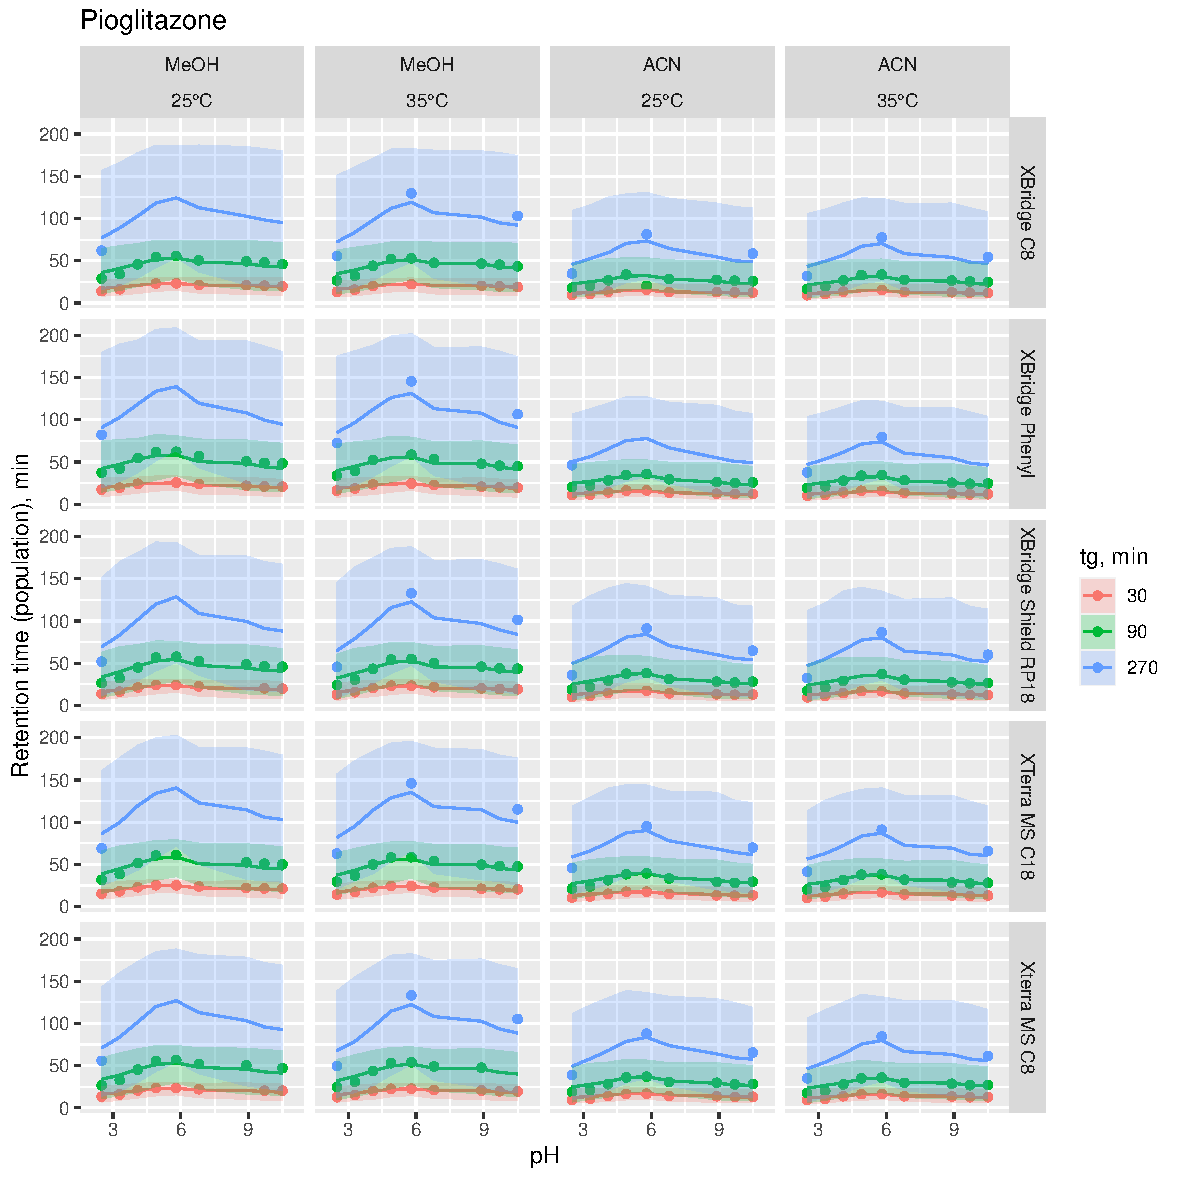
\includegraphics{../figures/concordanceplots/Pioglitazone.population.pdf}

\newpage{}

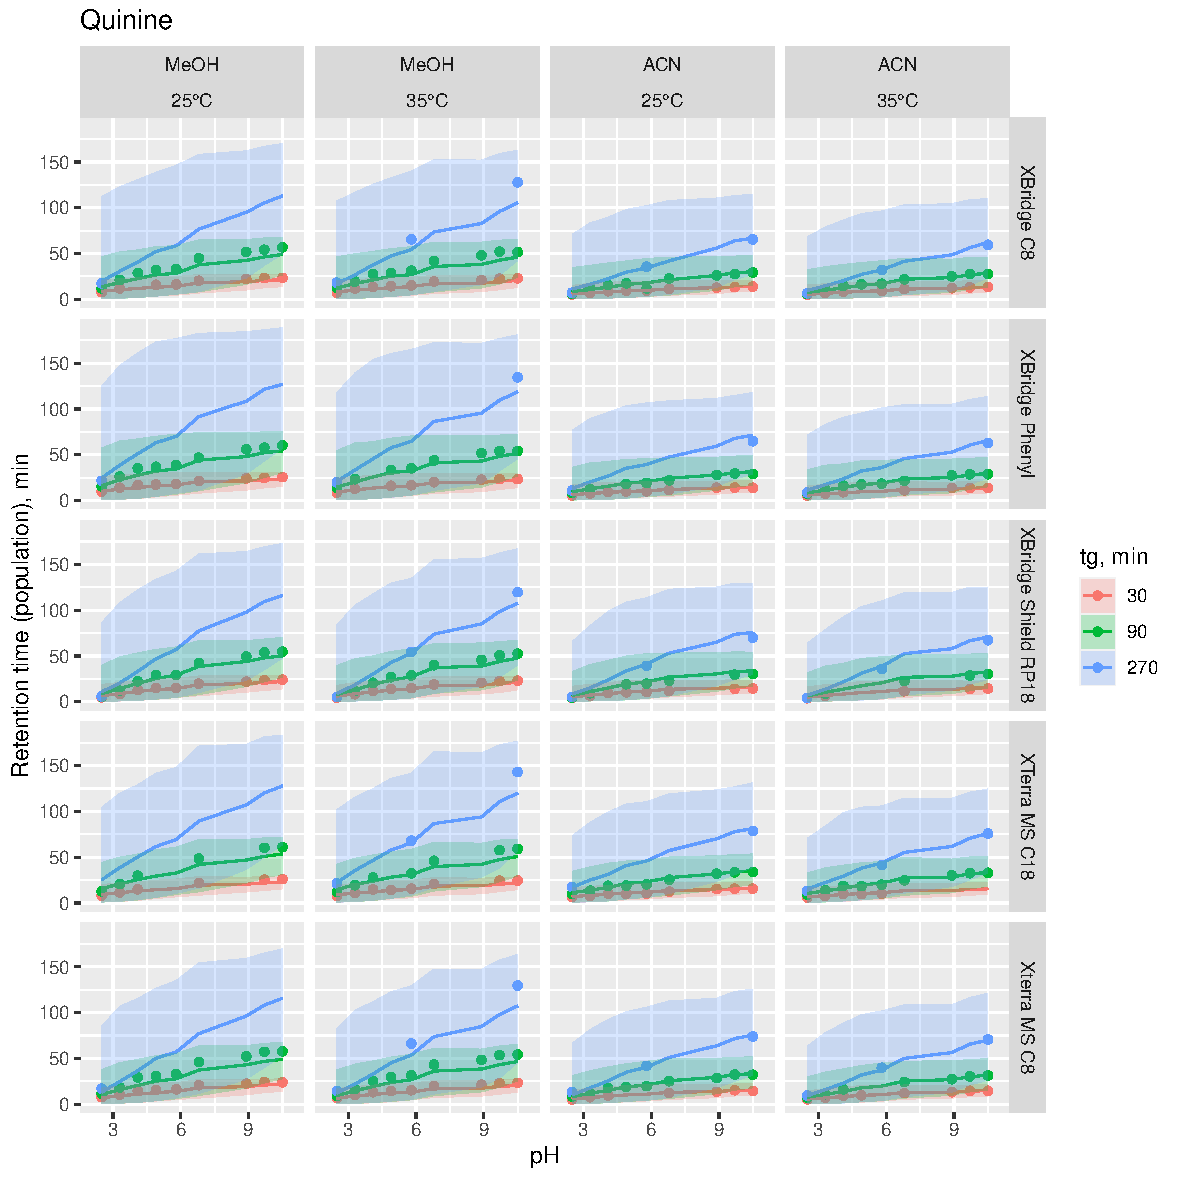
\includegraphics{../figures/concordanceplots/Quinine.population.pdf}

\newpage{}

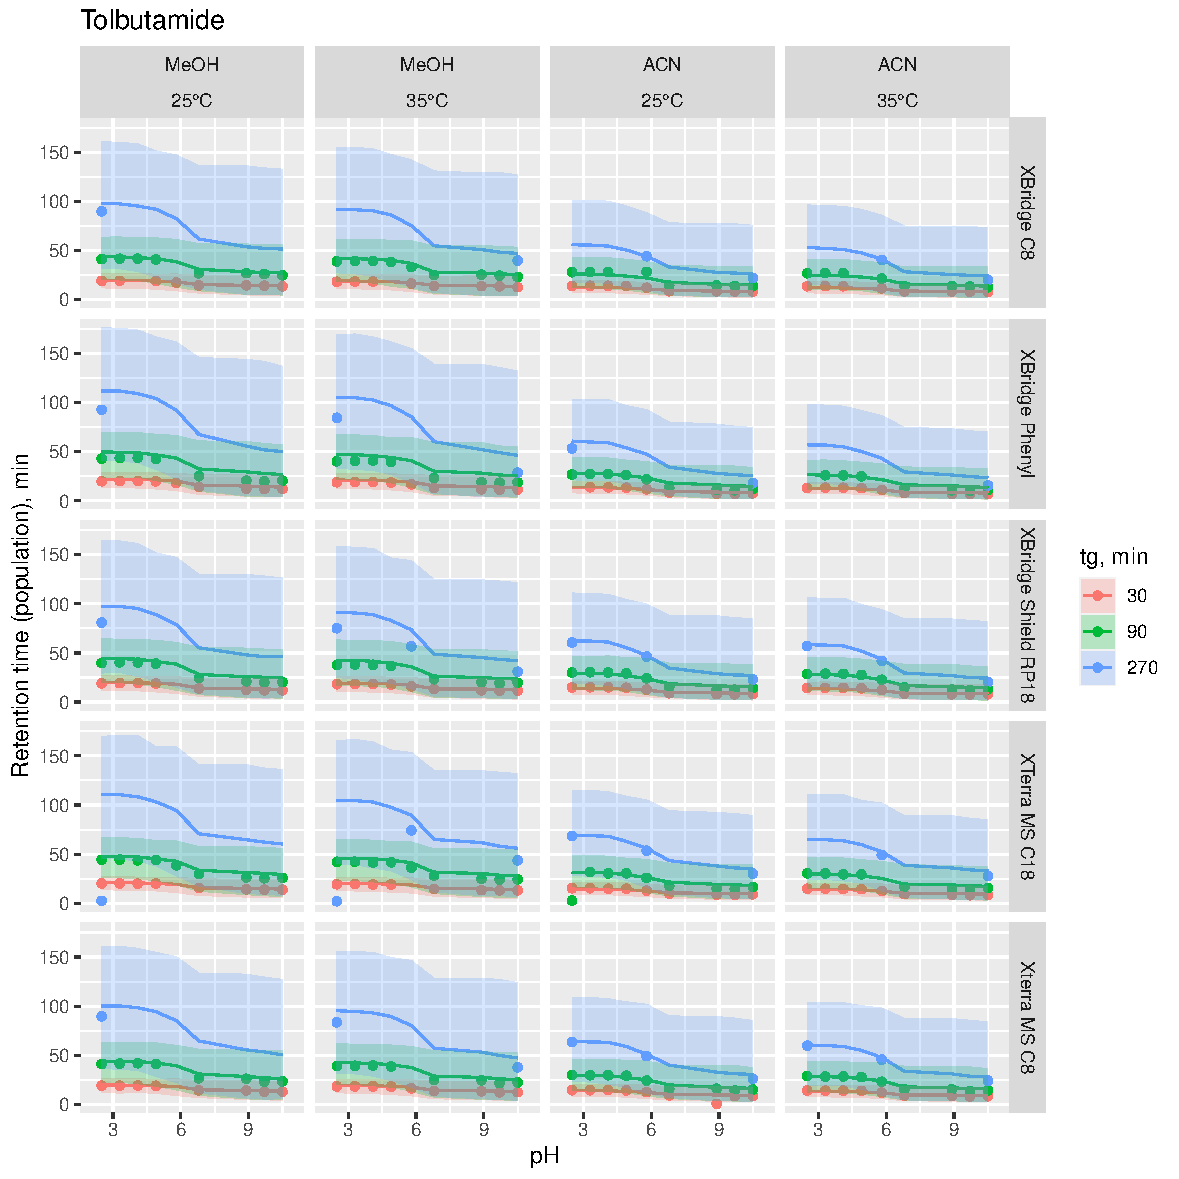
\includegraphics{../figures/concordanceplots/Tolbutamide.population.pdf}

\newpage{}

\hypertarget{figure-s6.-limited-data-gradient-predictions.}{%
\section{Figure S6. Limited data gradient
predictions.}\label{figure-s6.-limited-data-gradient-predictions.}}

Predictions represented as posterior median (line) and 5th-95th
percentiles (areas) for 6 exemplary analytes. Observed retention factors
are shown as dots. Predictions corresponding to future observations
given population-level parameters and predictors (logP and pKa), and
XBridge Shield RP18 data. Closed dotes represent data used for
predictions.

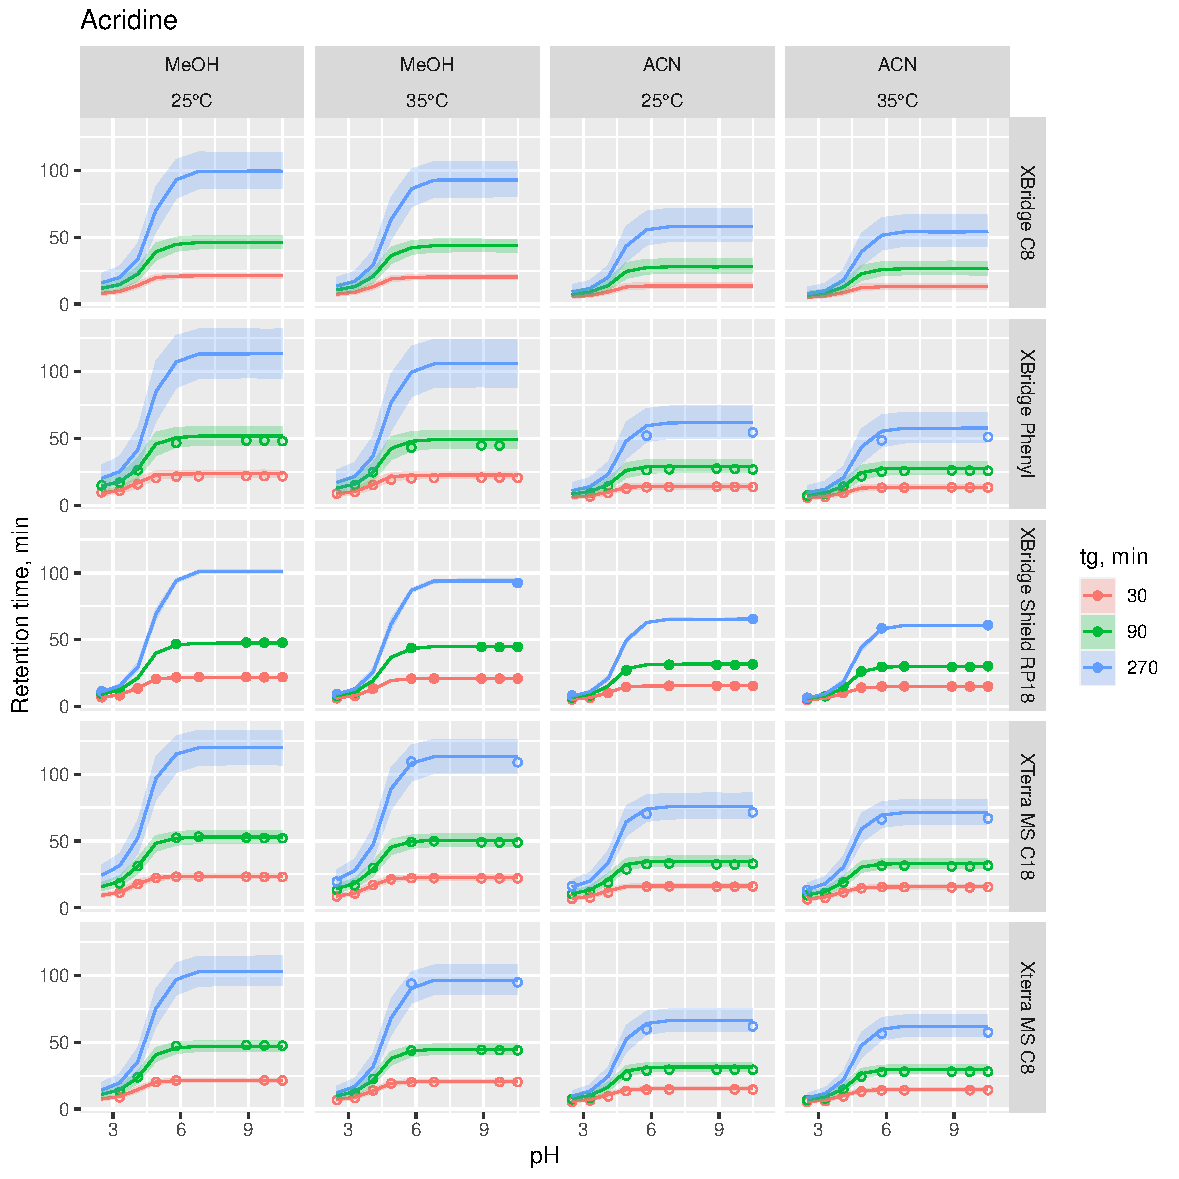
\includegraphics{../figures/casestudy2/concordanceplots/Acridine.pdf}

\newpage{}

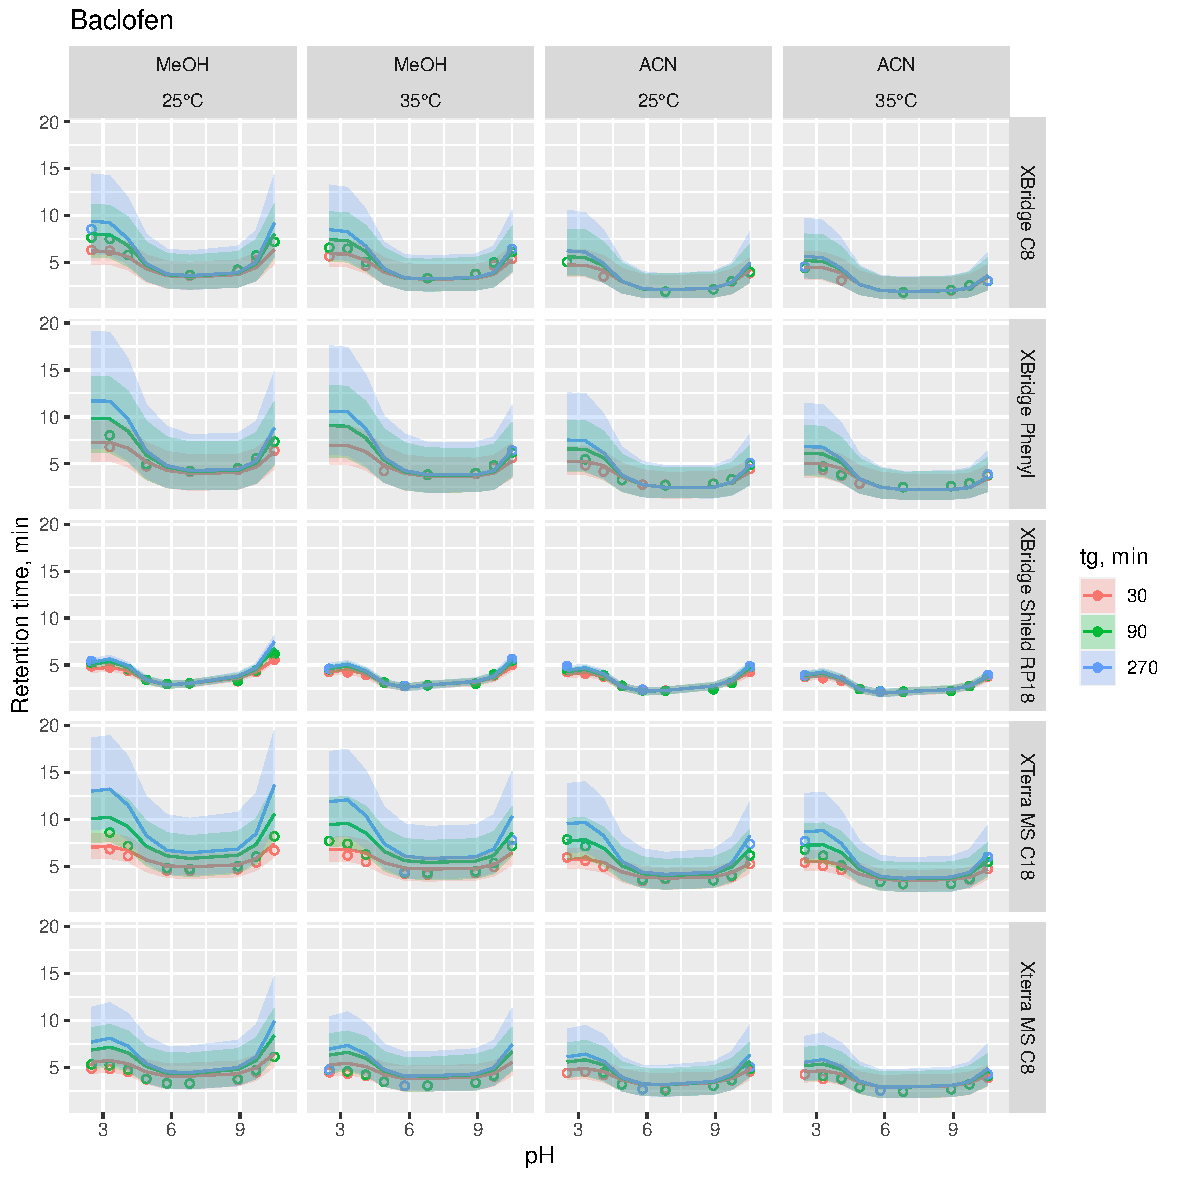
\includegraphics{../figures/casestudy2/concordanceplots/Baclofen.pdf}

\newpage{}

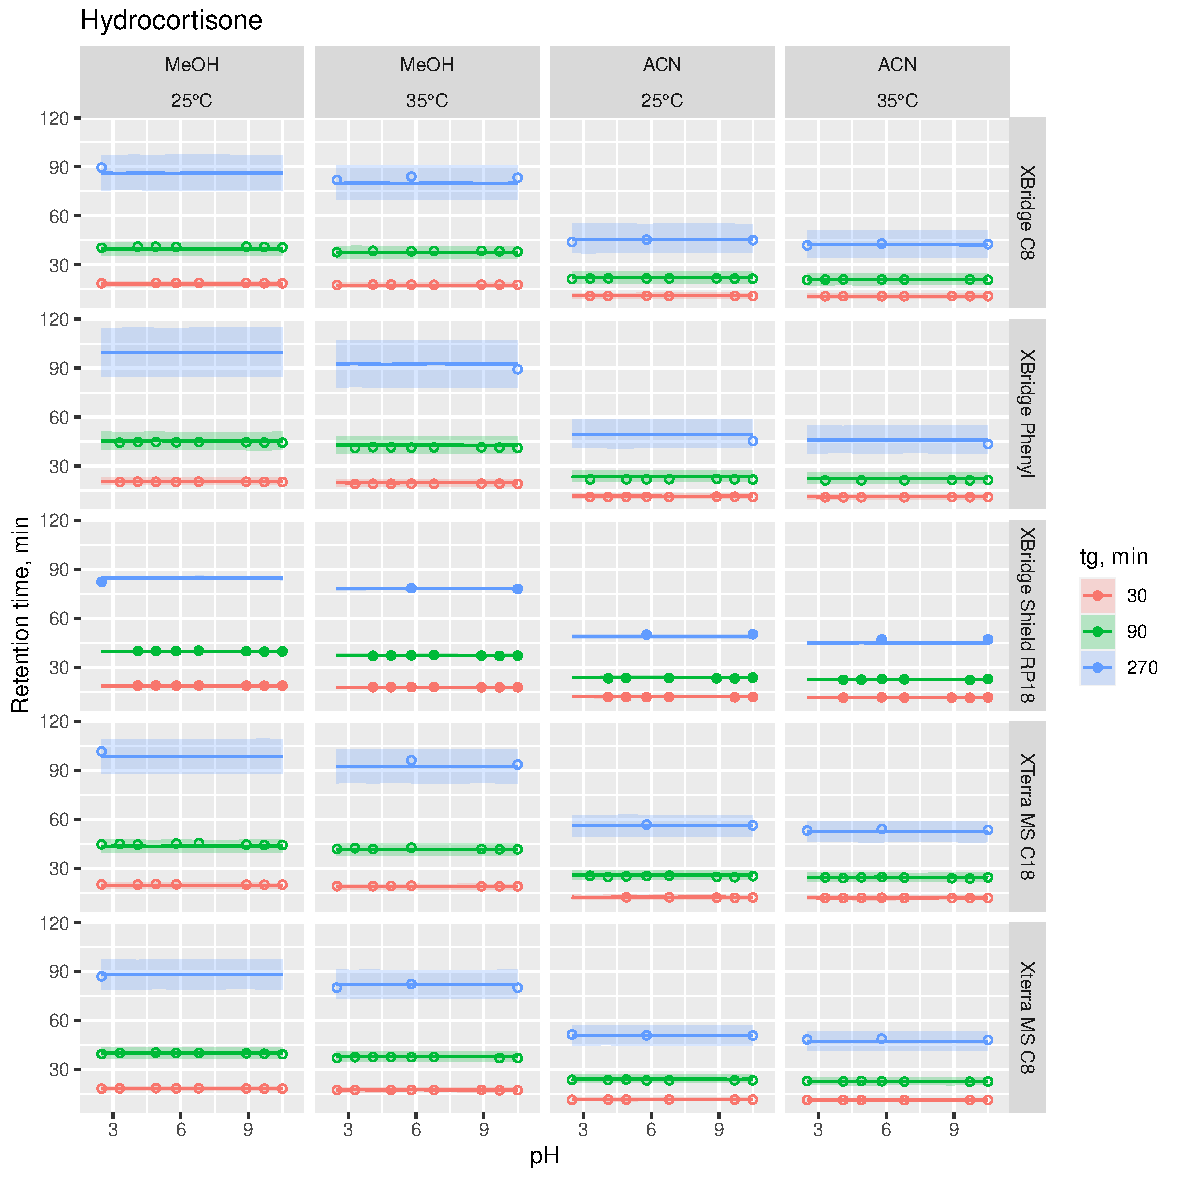
\includegraphics{../figures/casestudy2/concordanceplots/Hydrocortisone.pdf}

\newpage{}

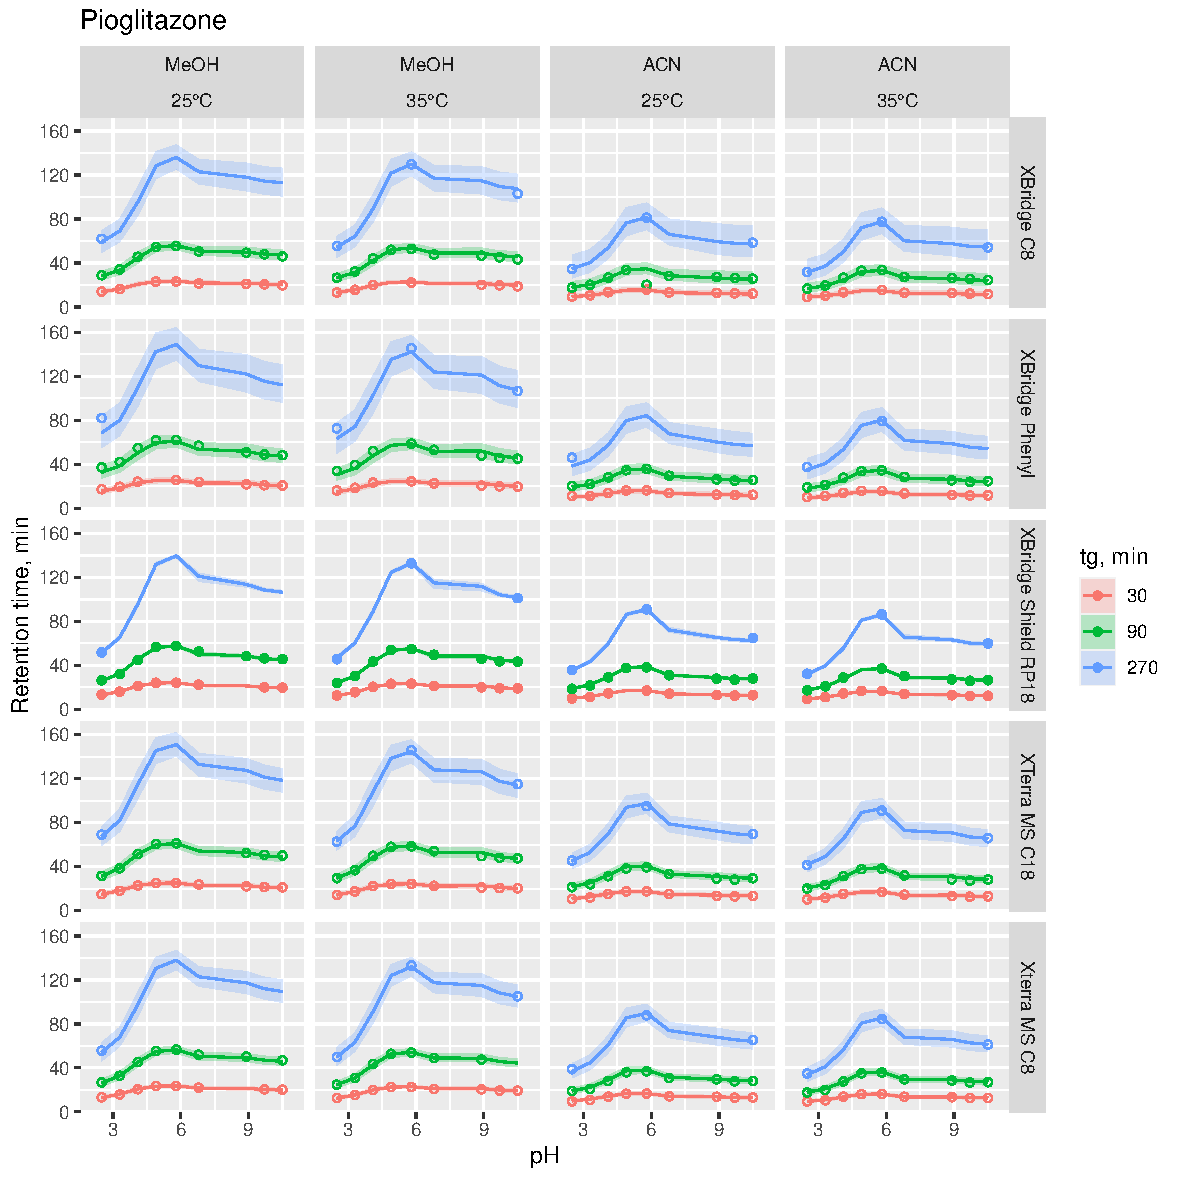
\includegraphics{../figures/casestudy2/concordanceplots/Pioglitazone.pdf}

\newpage{}

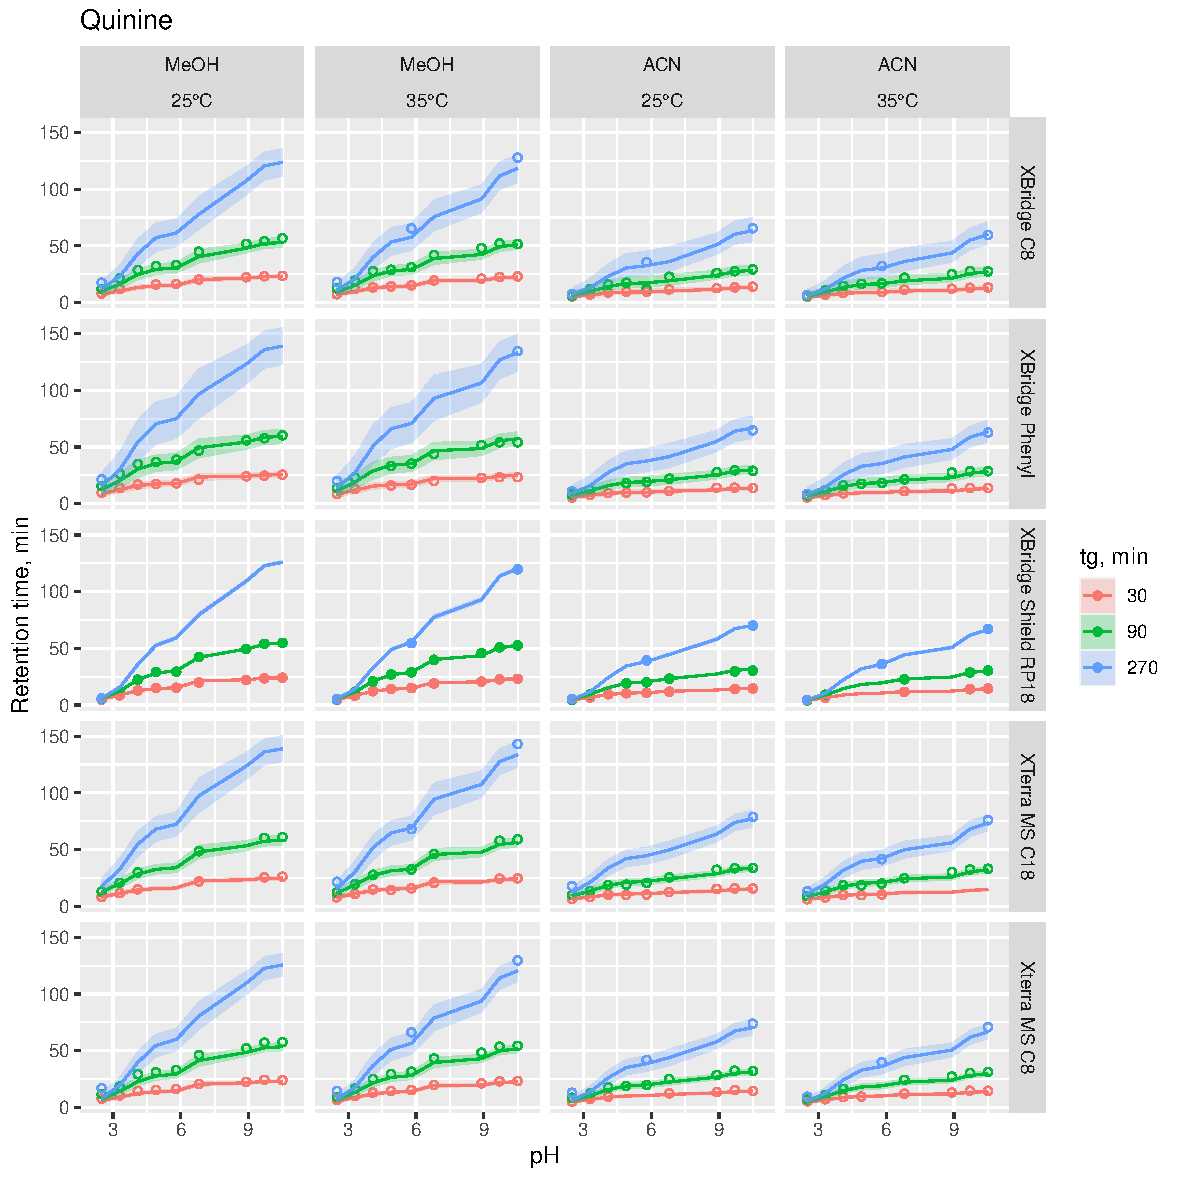
\includegraphics{../figures/casestudy2/concordanceplots/Quinine.pdf}

\newpage{}

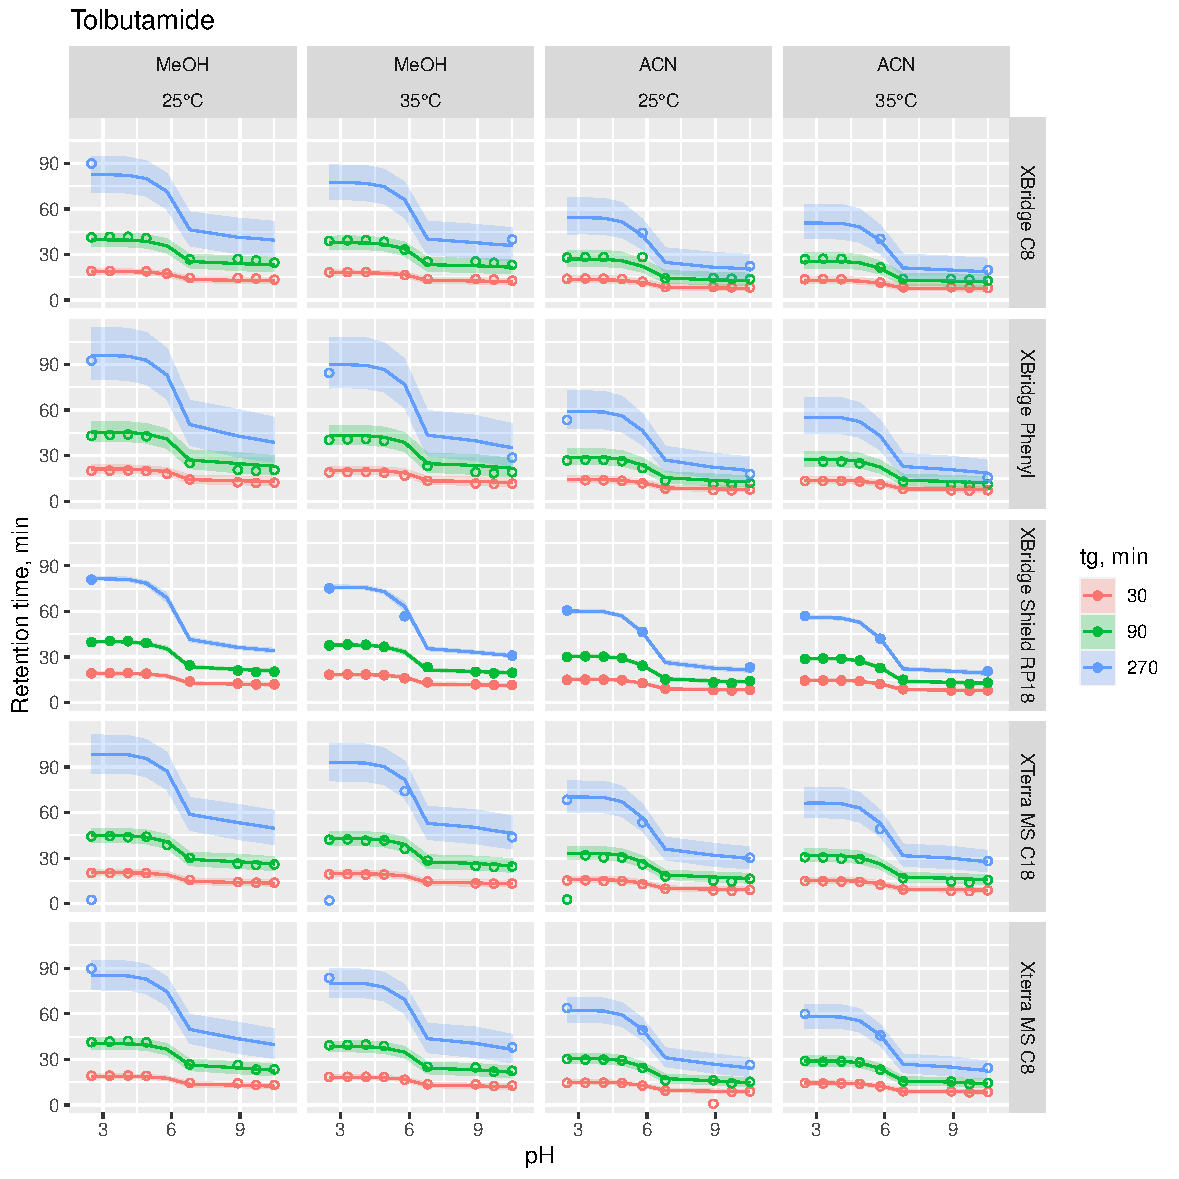
\includegraphics{../figures/casestudy2/concordanceplots/Tolbutamide.pdf}

\newpage{}

\hypertarget{figure-s7.-uncertainty-chromatograms.}{%
\section{Figure S7. Uncertainty
chromatograms.}\label{figure-s7.-uncertainty-chromatograms.}}

Uncertainty chromatograms displaying the predictions for 6 selected
analytes using individual, population and limited data predictions. Each
peak represents the range of analyte retention factors compatible with
prior and preliminary data. The chromatographic conditions are pHo=8.9,
ACN, 25oC, tg = 90 min.

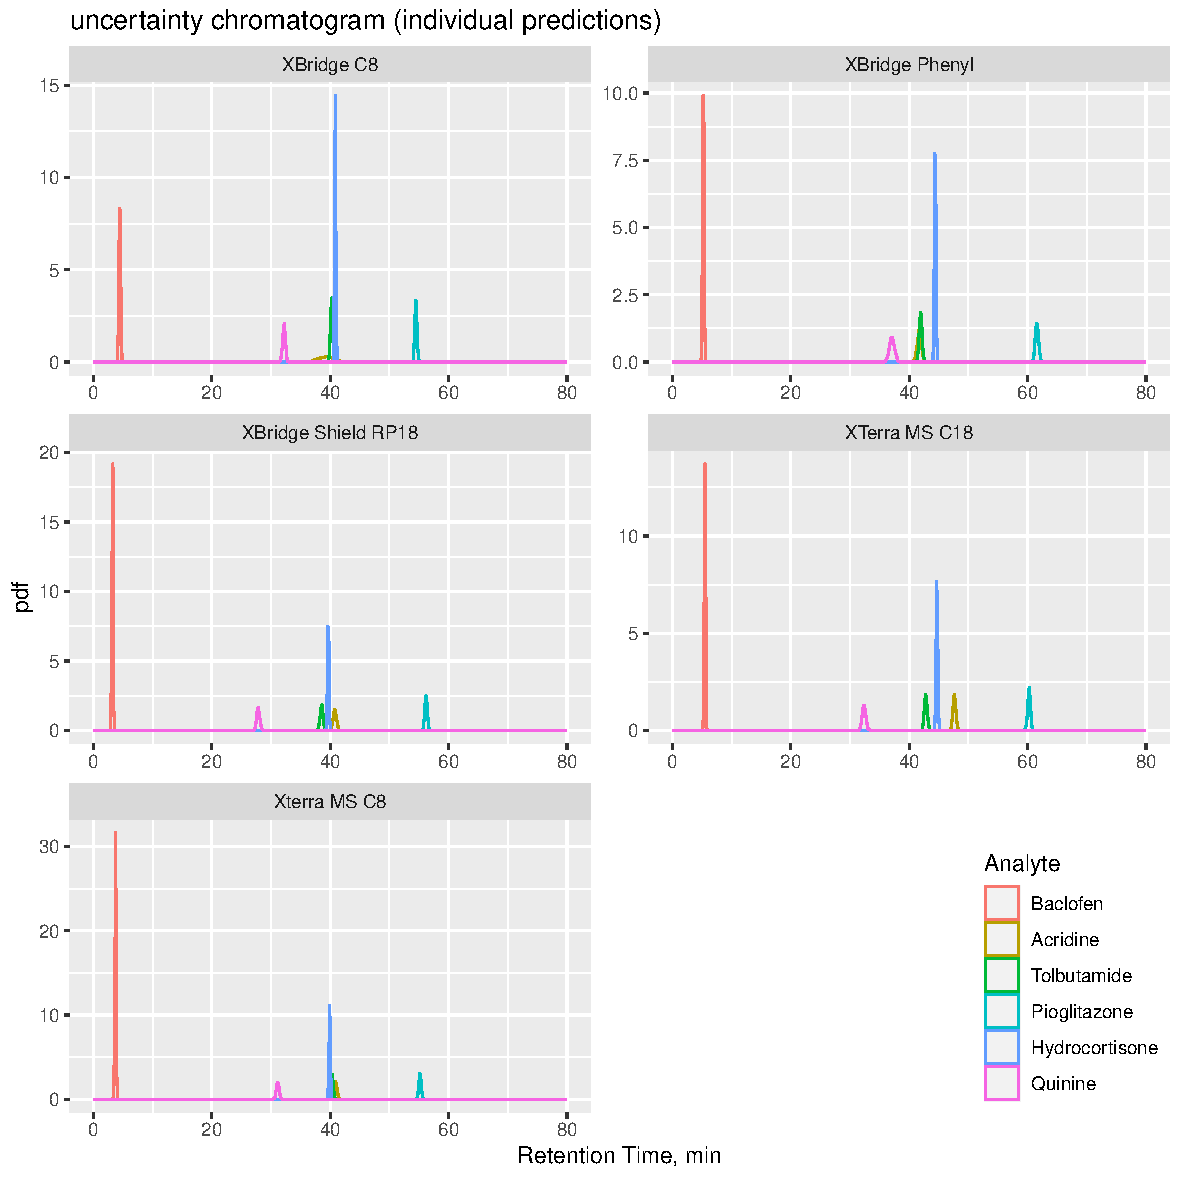
\includegraphics{../figures/concordanceplots/uncertainitychromatogram.individual.pdf}

\newpage{}

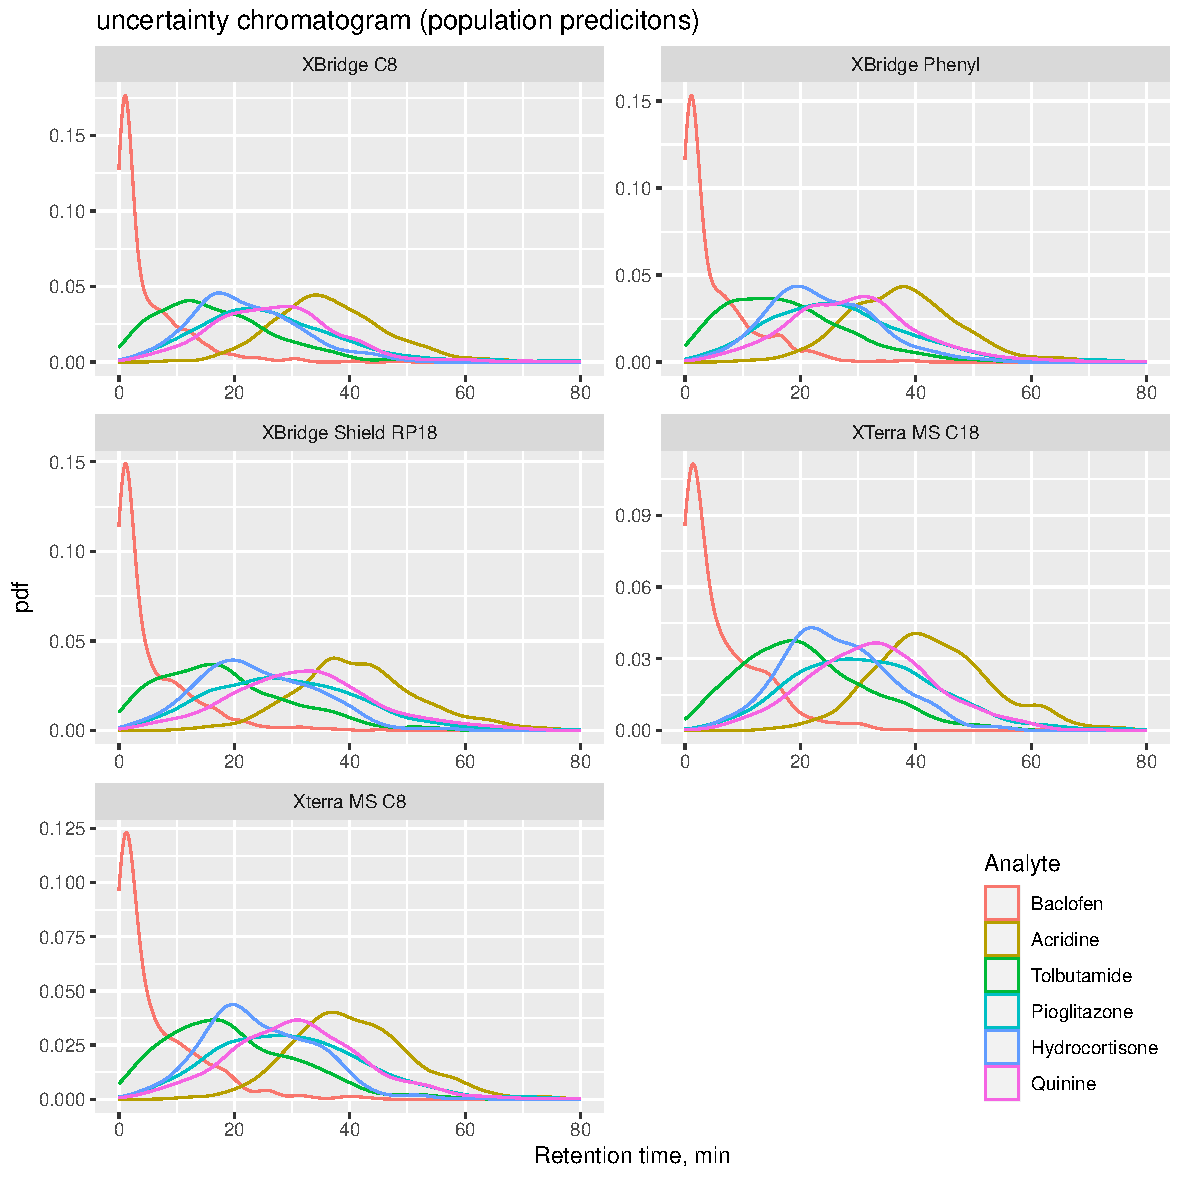
\includegraphics{../figures/concordanceplots/uncertainitychromatogram.population.pdf}

\newpage{}

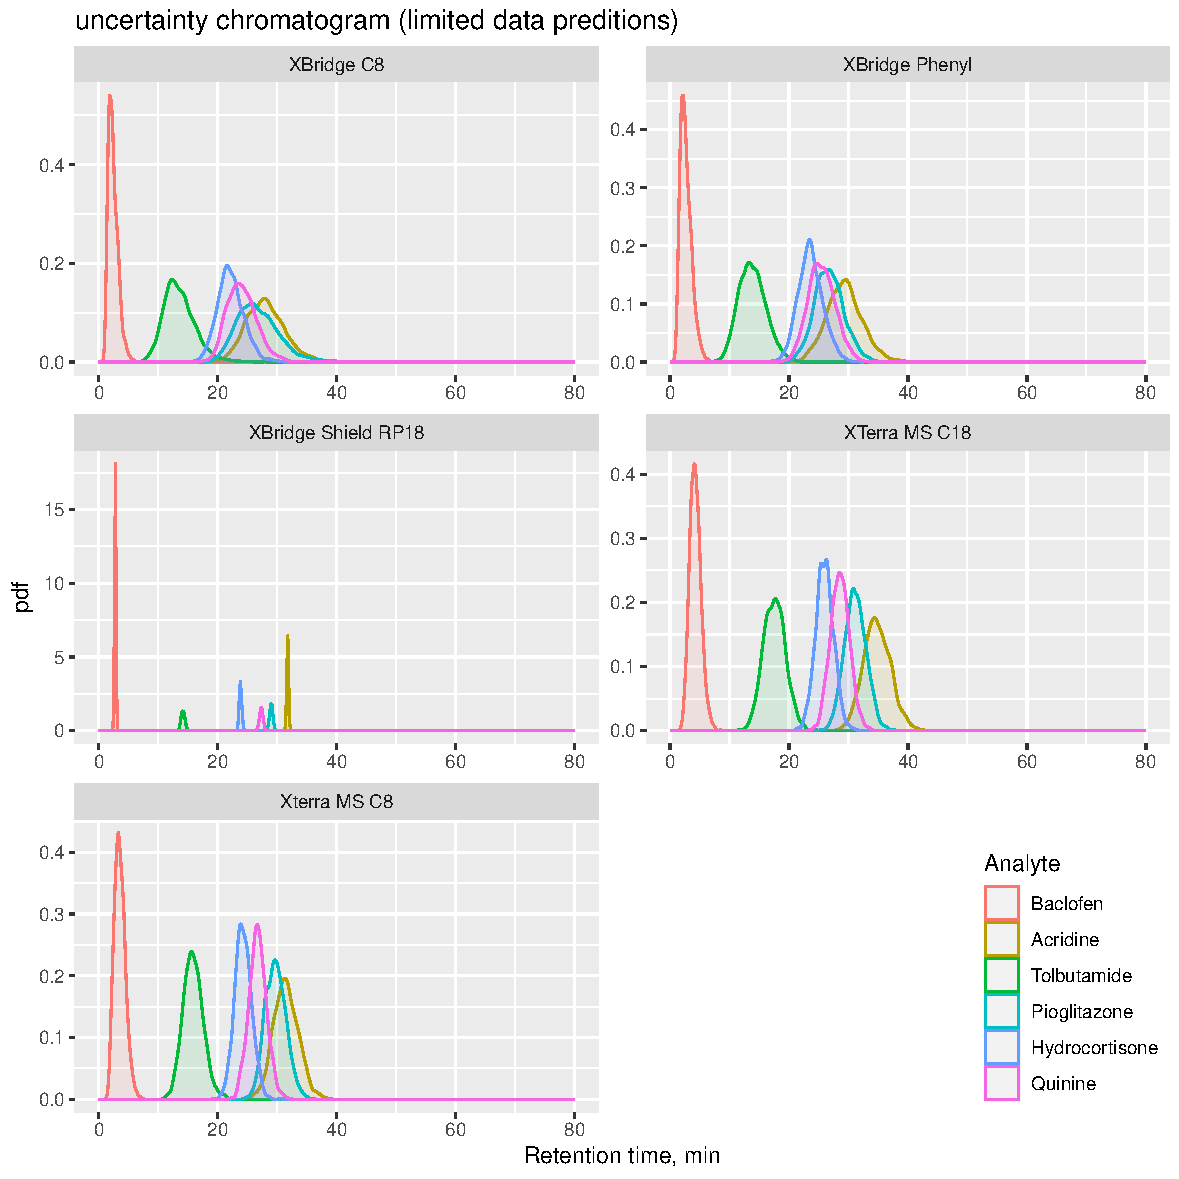
\includegraphics{../figures/casestudy2/concordanceplots/chromatogram.pdf}

\newpage{}

\hypertarget{figure-s8.-individual-izocratic-predictions.}{%
\section{Figure S8. Individual izocratic
predictions.}\label{figure-s8.-individual-izocratic-predictions.}}

Predictions represented as posterior median (line) and 5th-95th
percentiles (areas) for a 6 exemplary analytes. Predictions
corresponding to future observations given the population-level
parameters and all the retention data measured for a particular analyte.

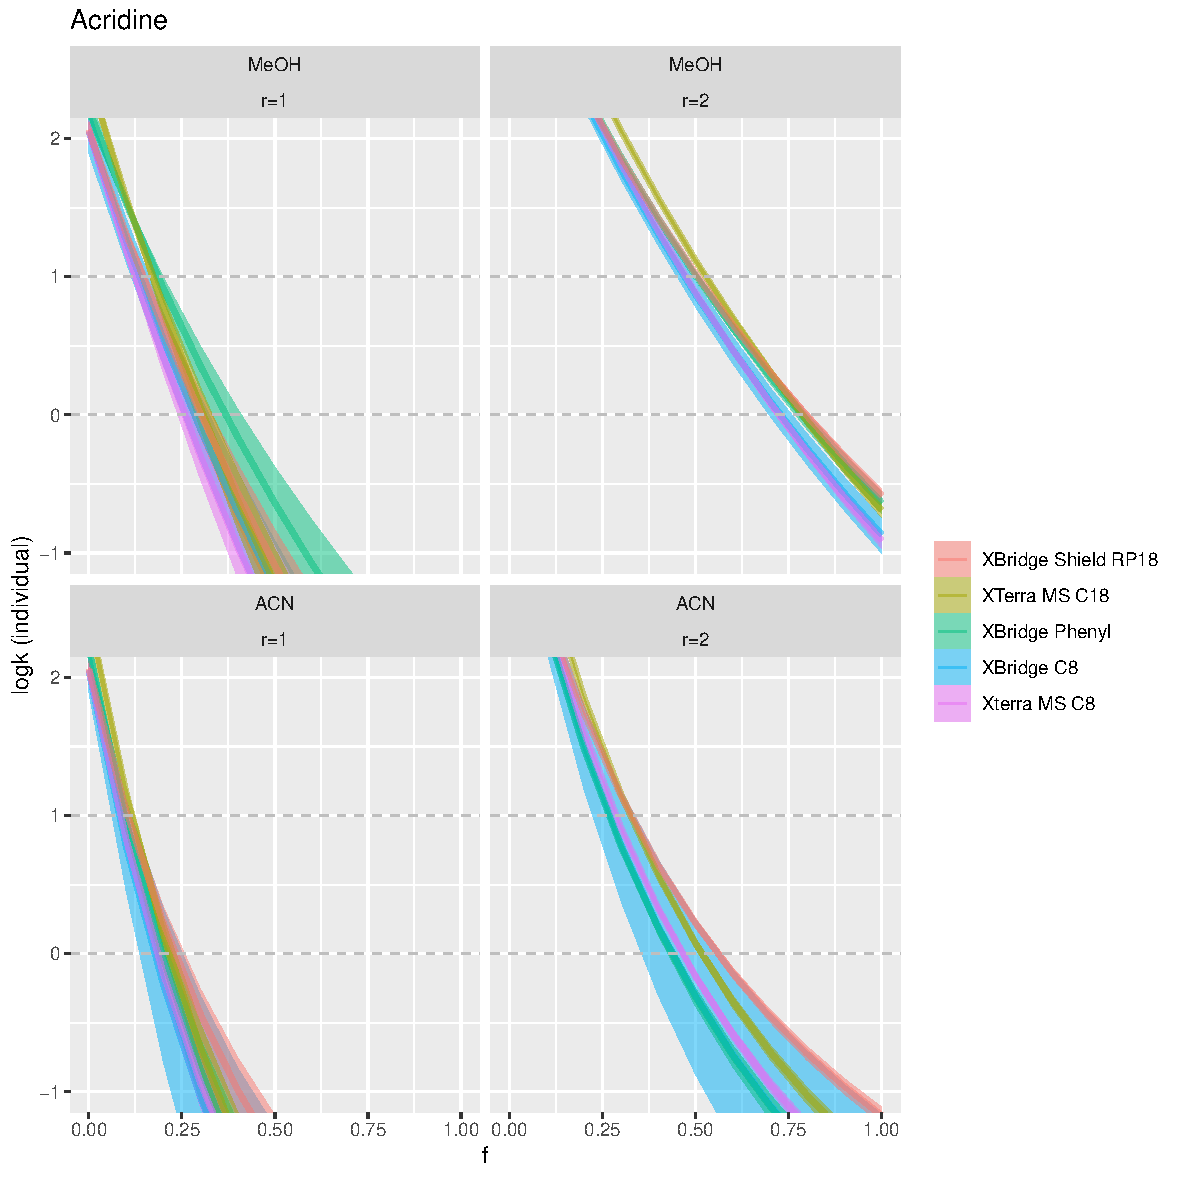
\includegraphics{../figures/izoparam/isopred/Acridine.individual.pdf}

\newpage{}

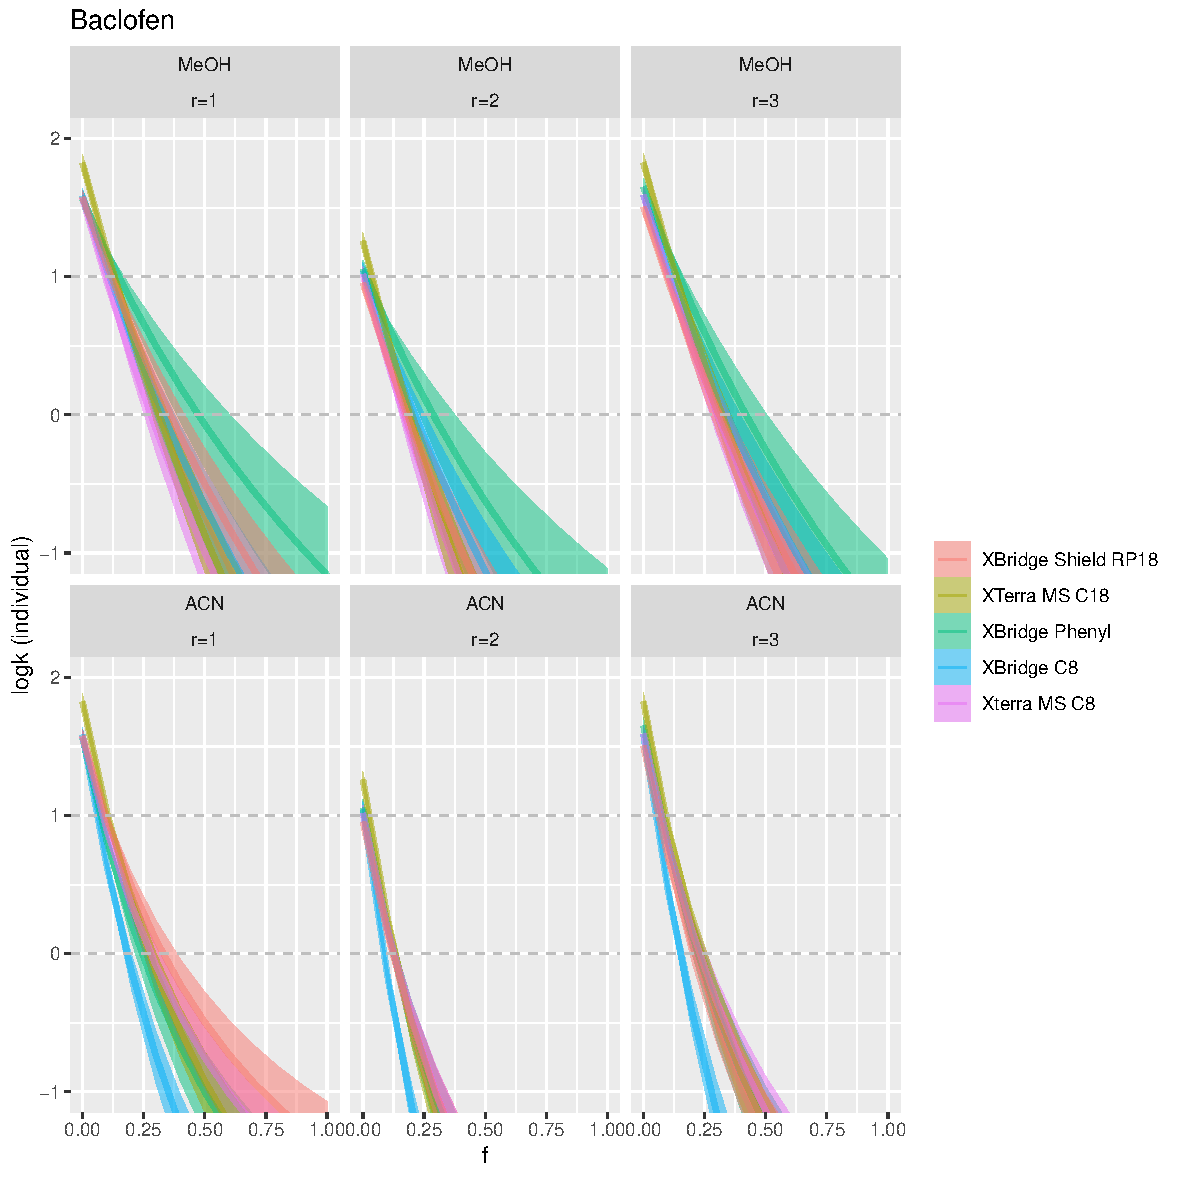
\includegraphics{../figures/izoparam/isopred/Baclofen.individual.pdf}

\newpage{}

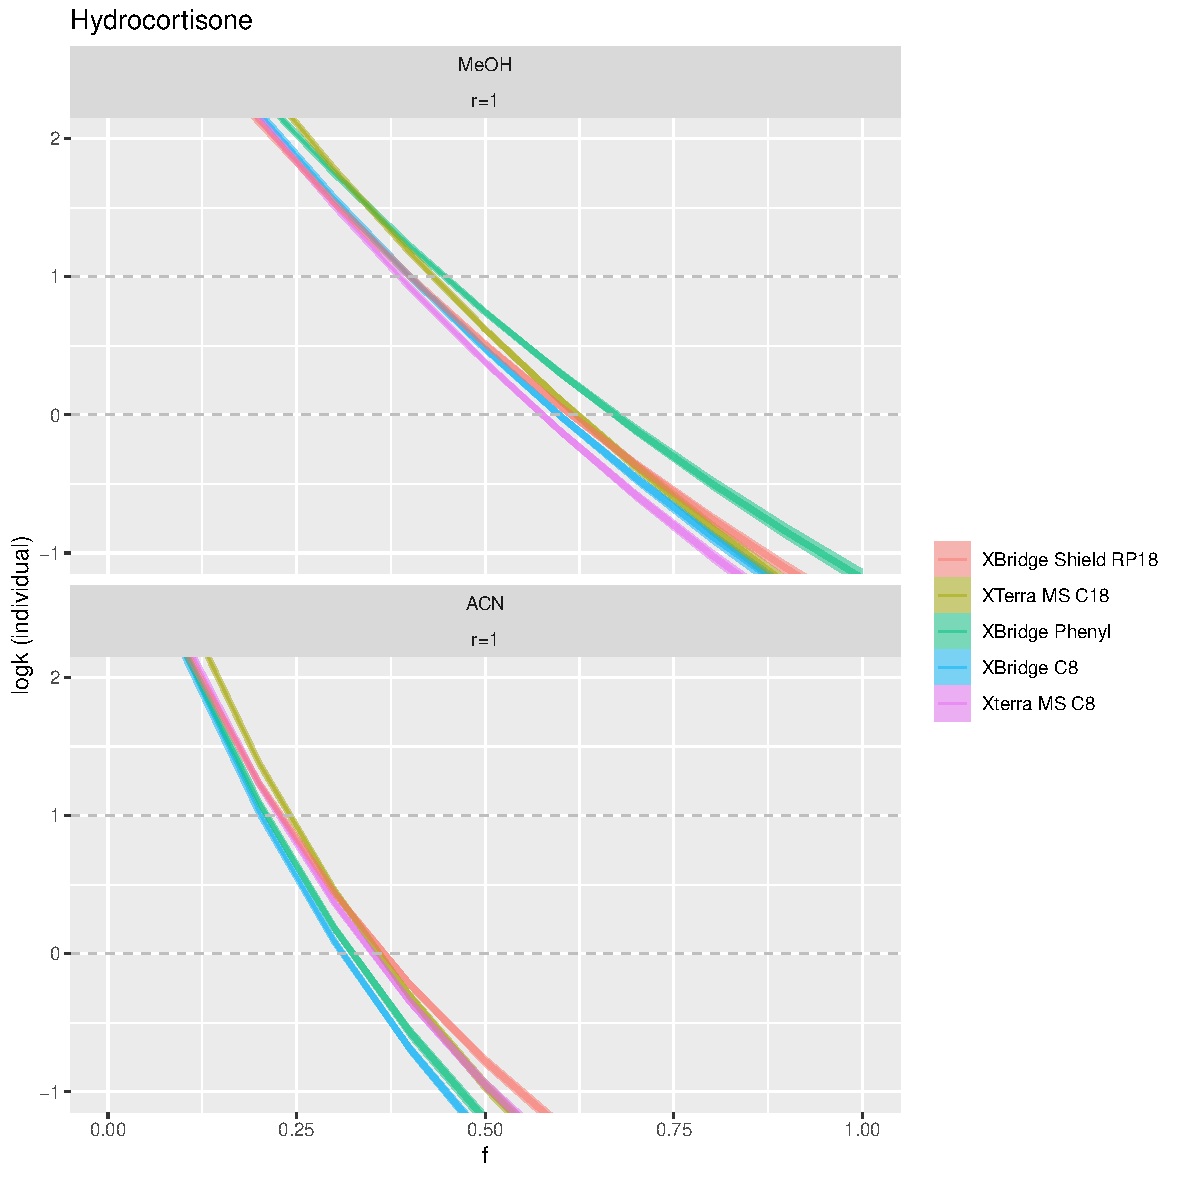
\includegraphics{../figures/izoparam/isopred/Hydrocortisone.individual.pdf}

\newpage{}

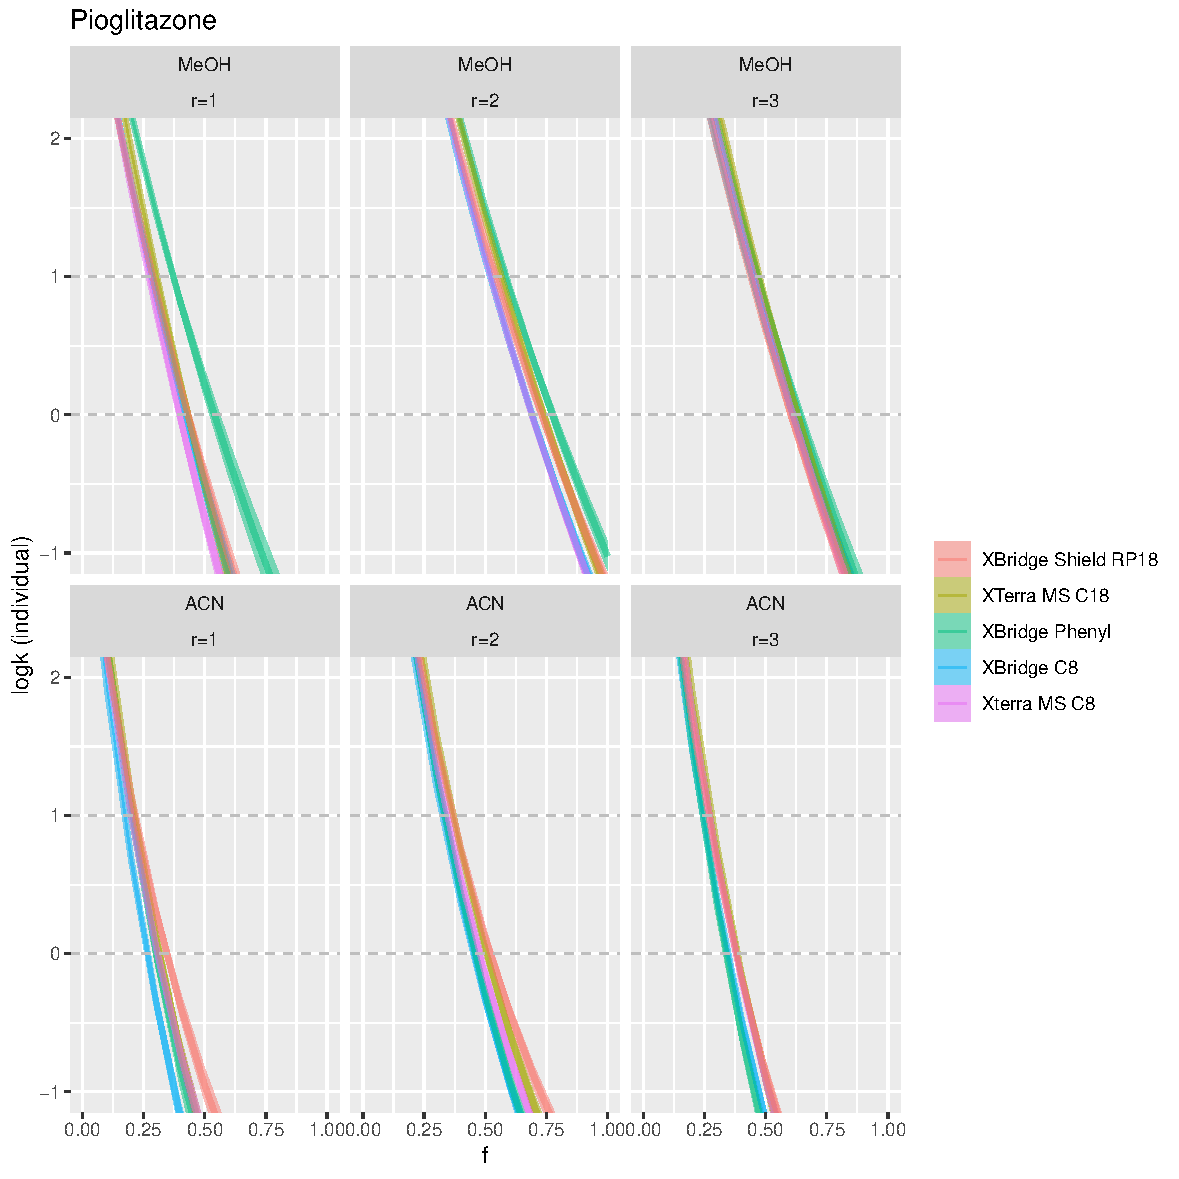
\includegraphics{../figures/izoparam/isopred/Pioglitazone.individual.pdf}

\newpage{}

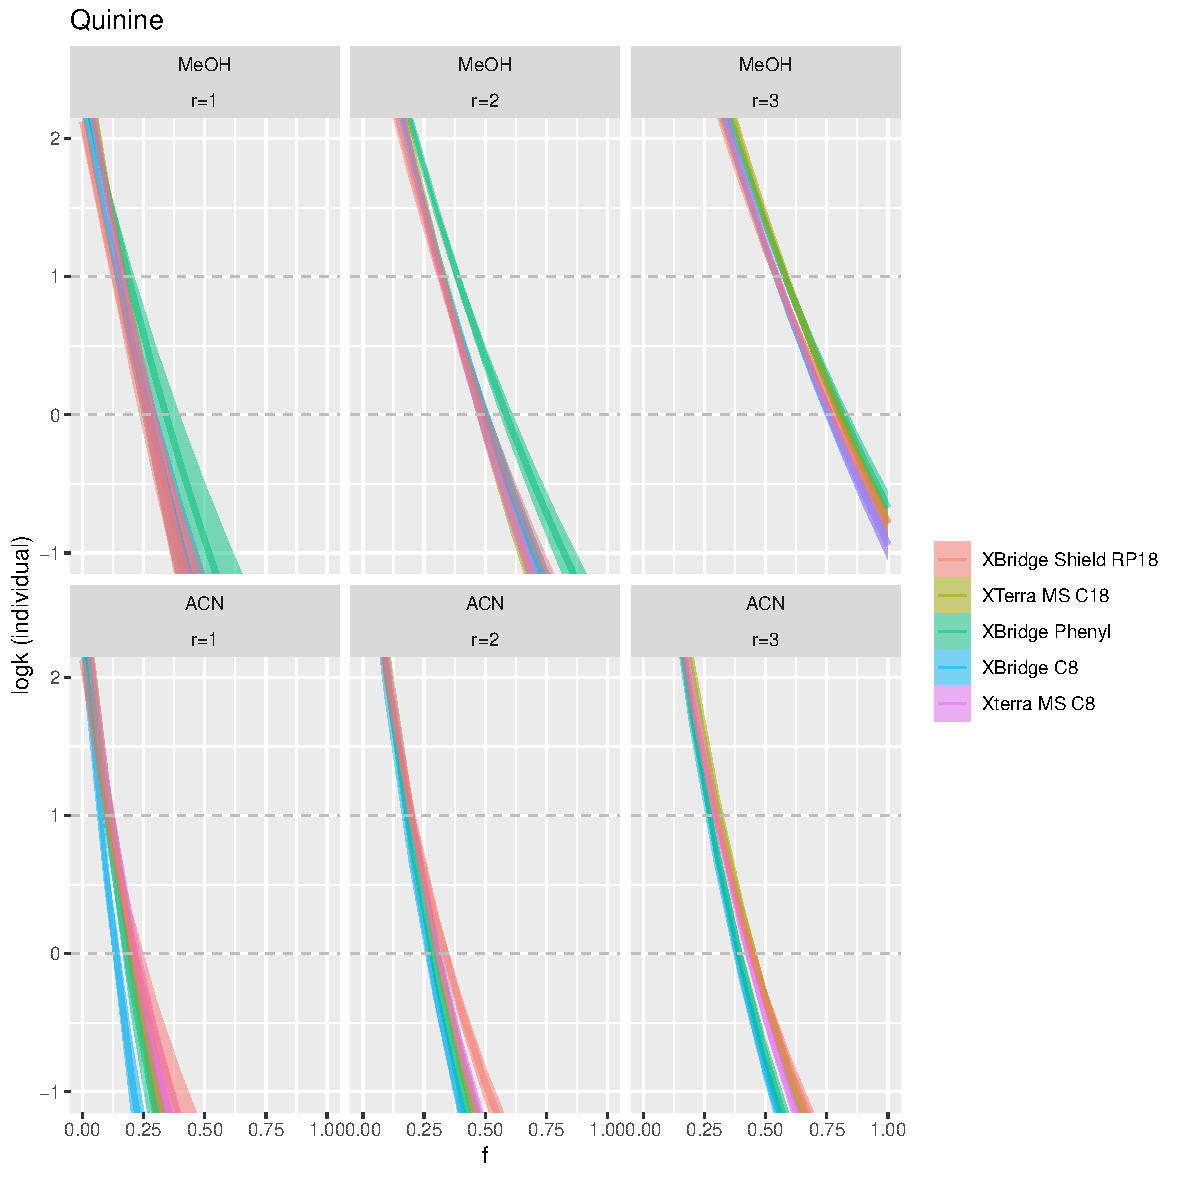
\includegraphics{../figures/izoparam/isopred/Quinine.individual.pdf}

\newpage{}

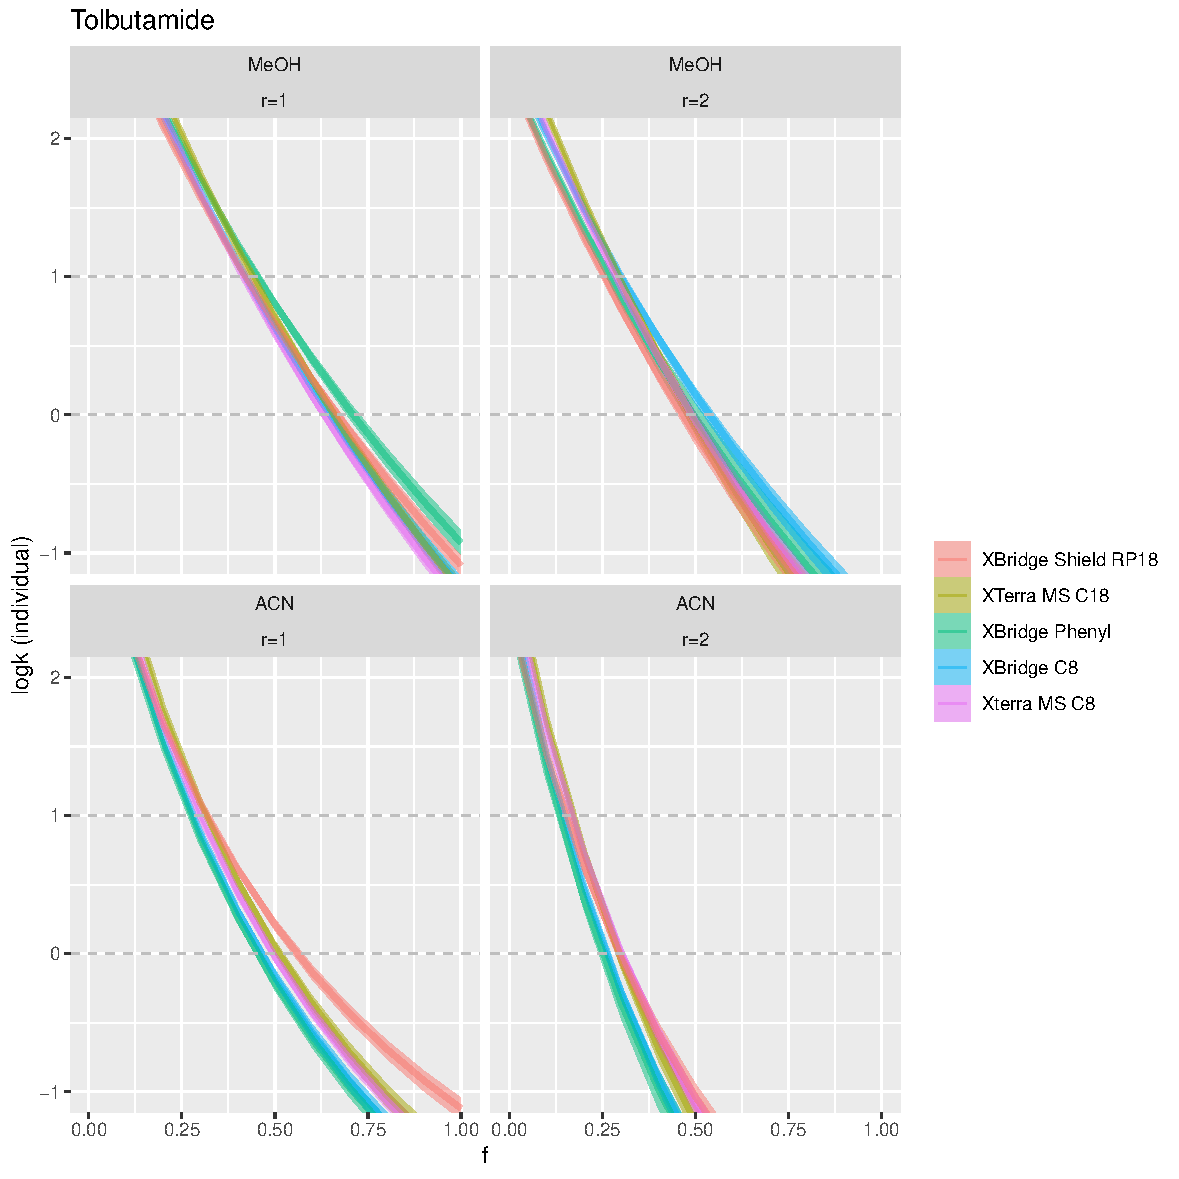
\includegraphics{../figures/izoparam/isopred/Tolbutamide.individual.pdf}

\newpage{}

\hypertarget{figure-s9.-population-isocratic-predictions.}{%
\section{Figure S9. Population isocratic
predictions.}\label{figure-s9.-population-isocratic-predictions.}}

Predictions represented as posterior median (line) and 5th-95th
percentiles (areas) for a 6 exemplary analytes. Predictions
corresponding to future observations given only population-level
parameters and predictors (logP and pKa).

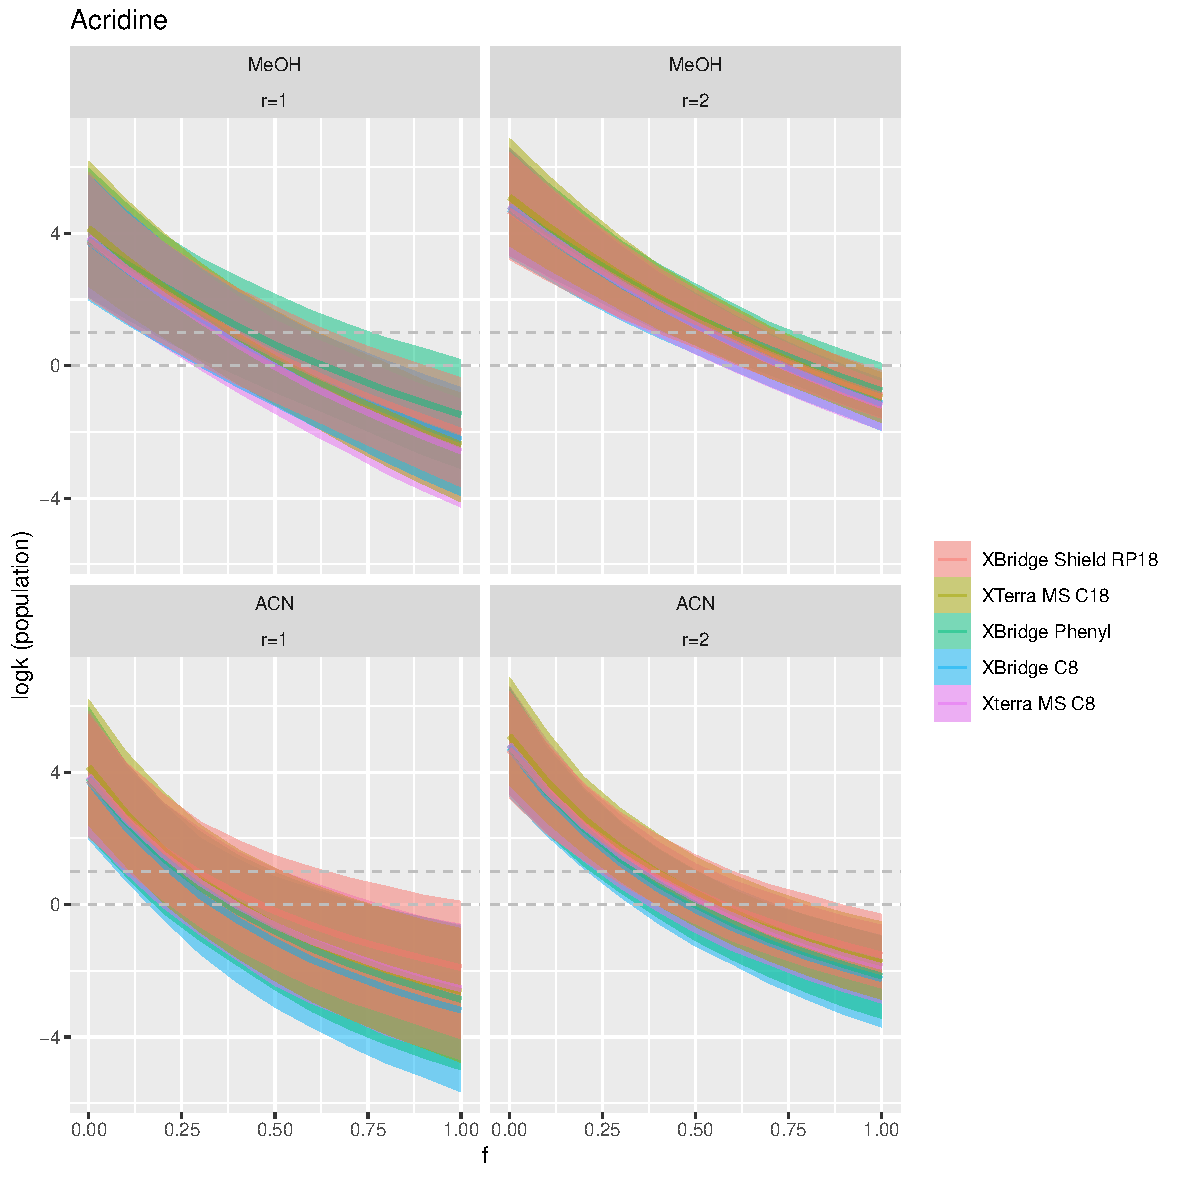
\includegraphics{../figures/izoparam/isopred/Acridine.population.pdf}

\newpage{}

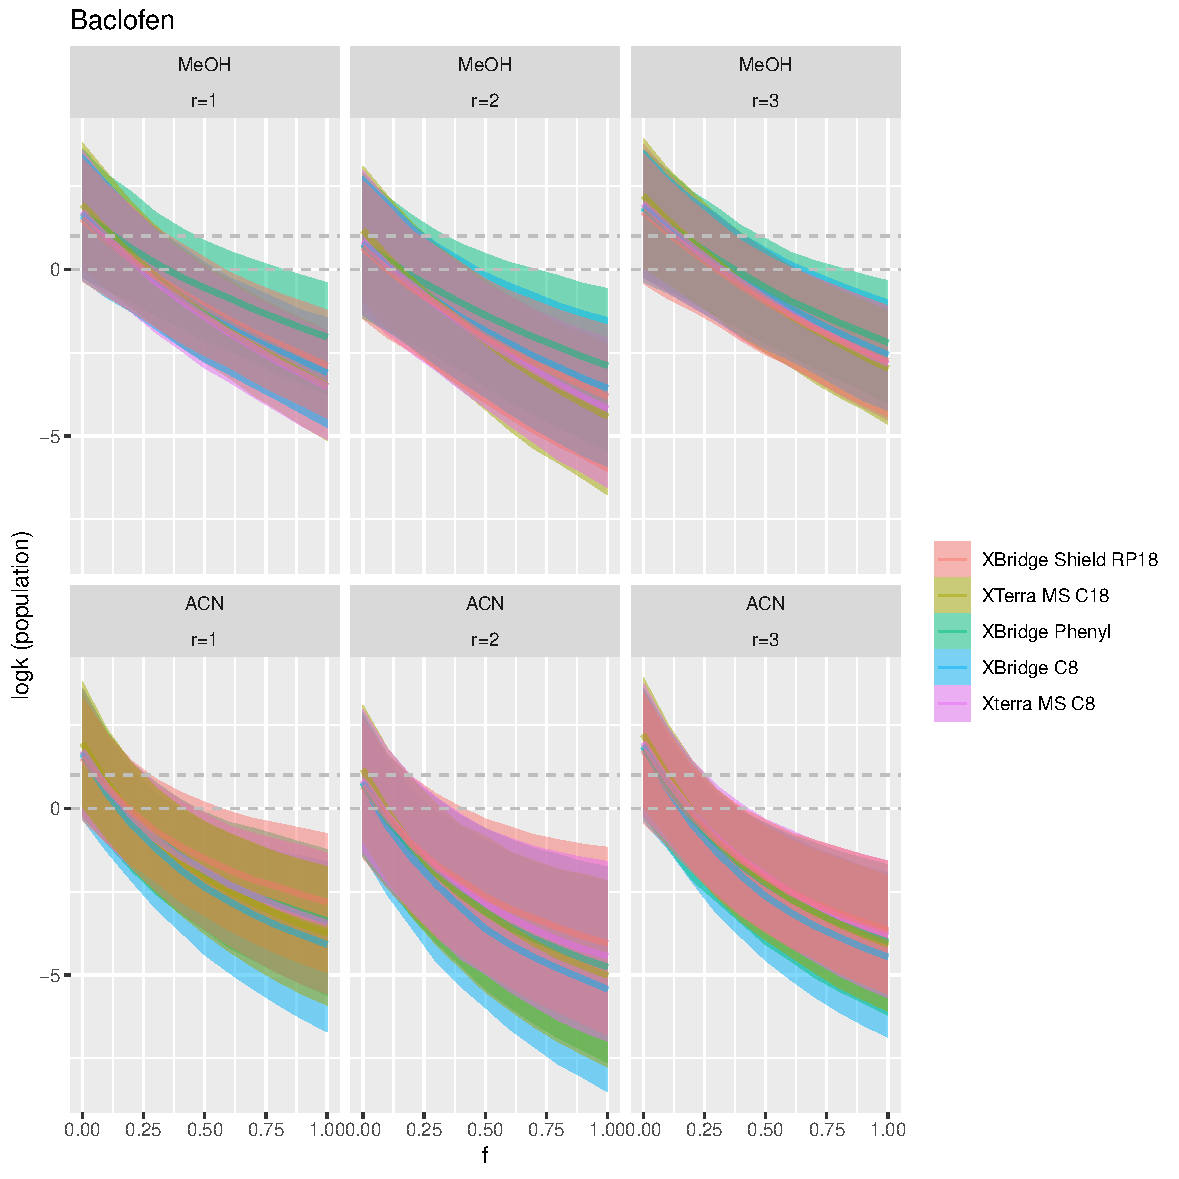
\includegraphics{../figures/izoparam/isopred/Baclofen.population.pdf}

\newpage{}

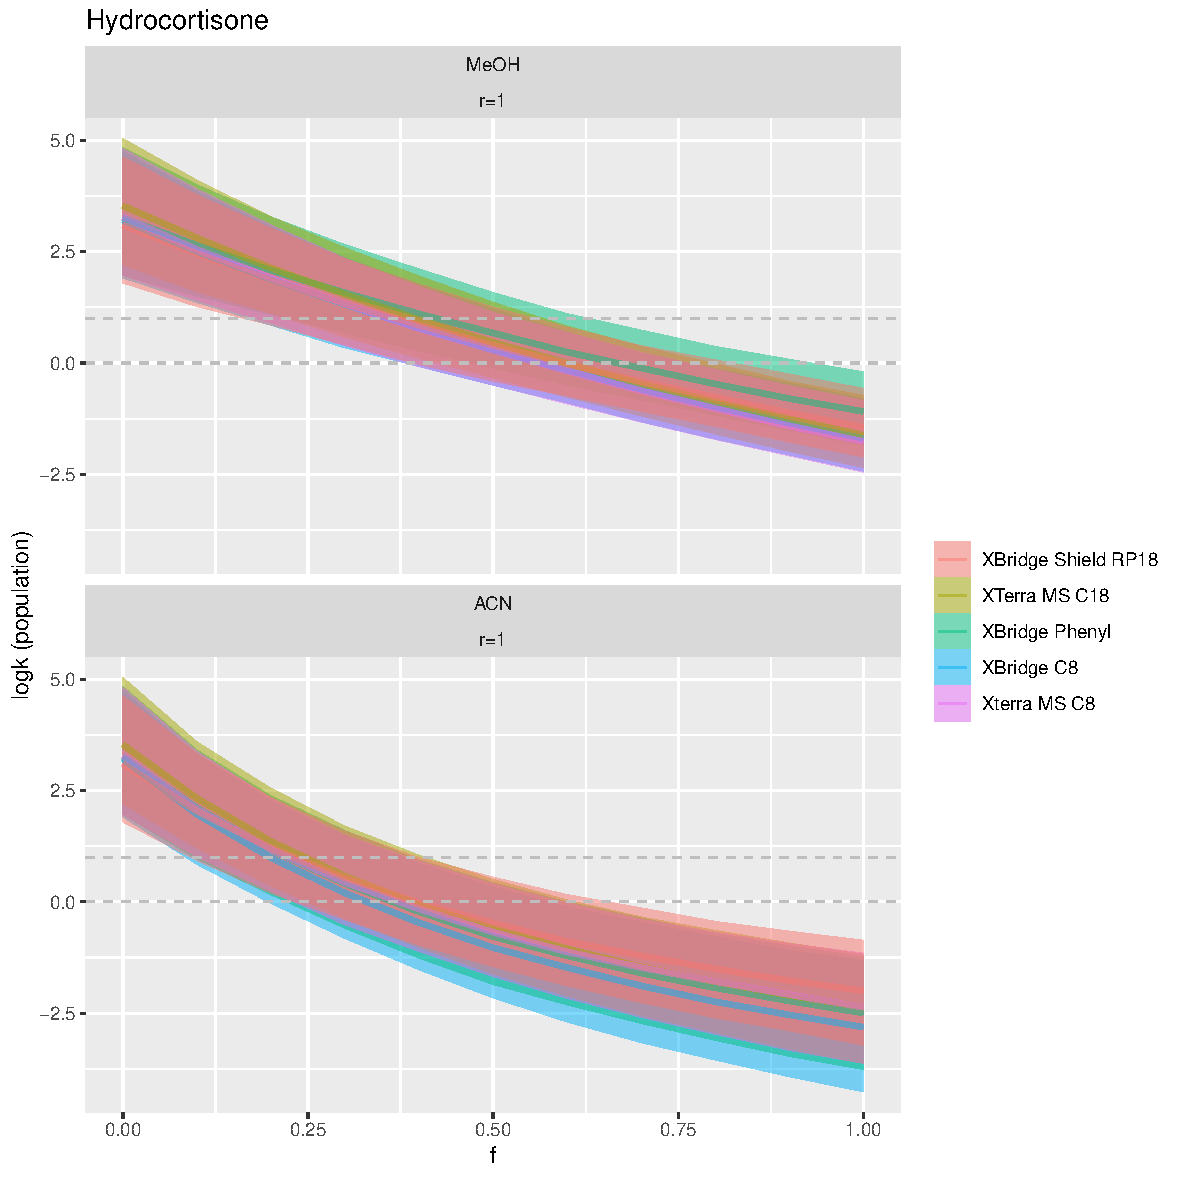
\includegraphics{../figures/izoparam/isopred/Hydrocortisone.population.pdf}

\newpage{}

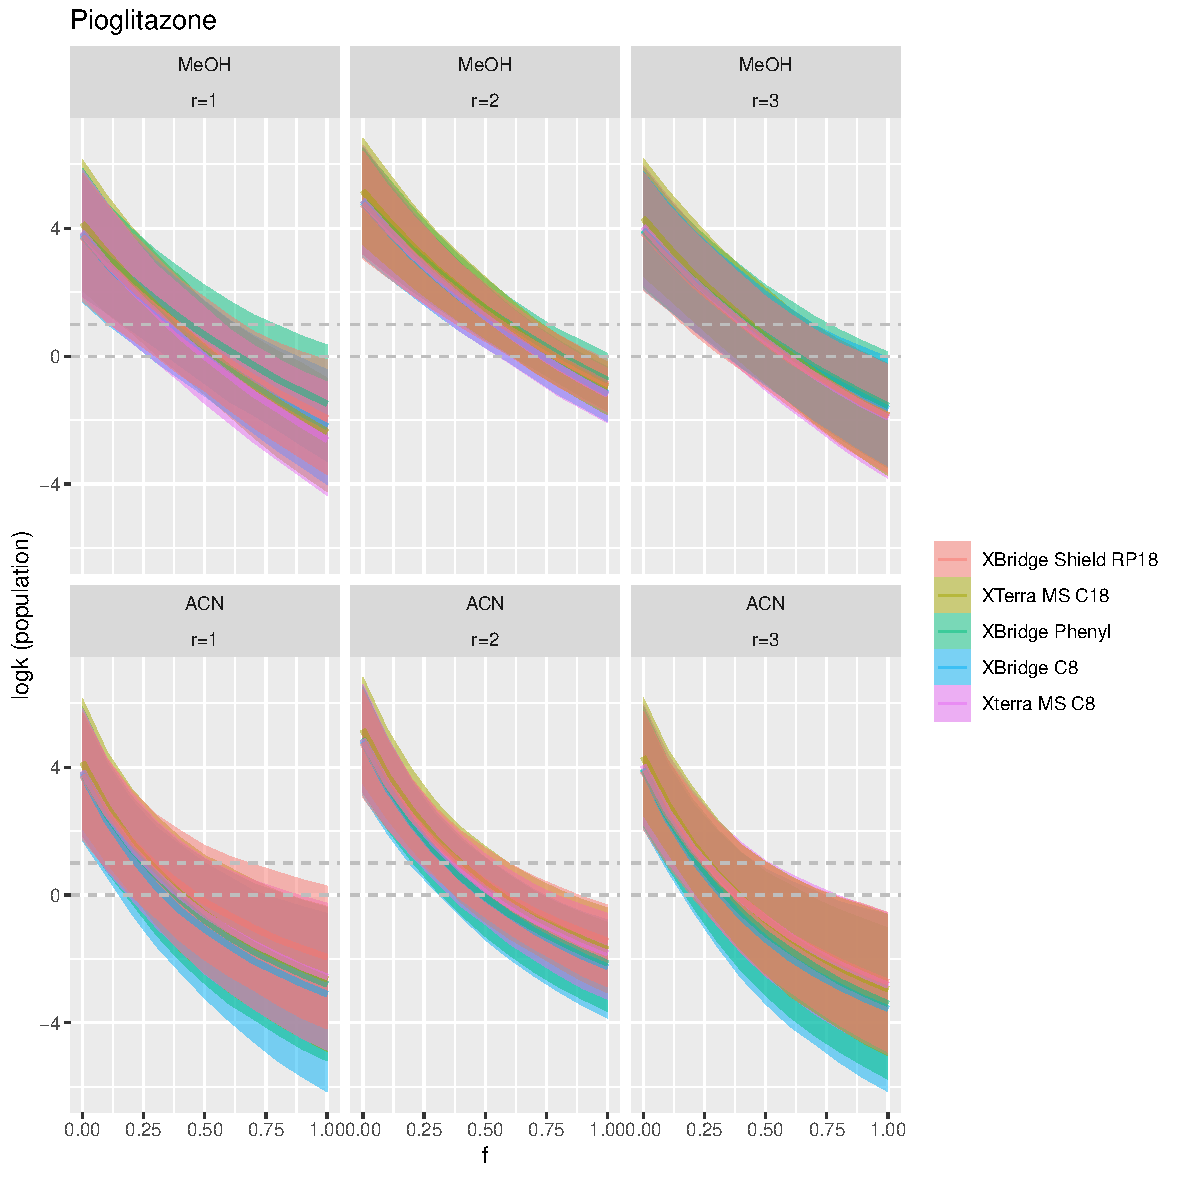
\includegraphics{../figures/izoparam/isopred/Pioglitazone.population.pdf}

\newpage{}

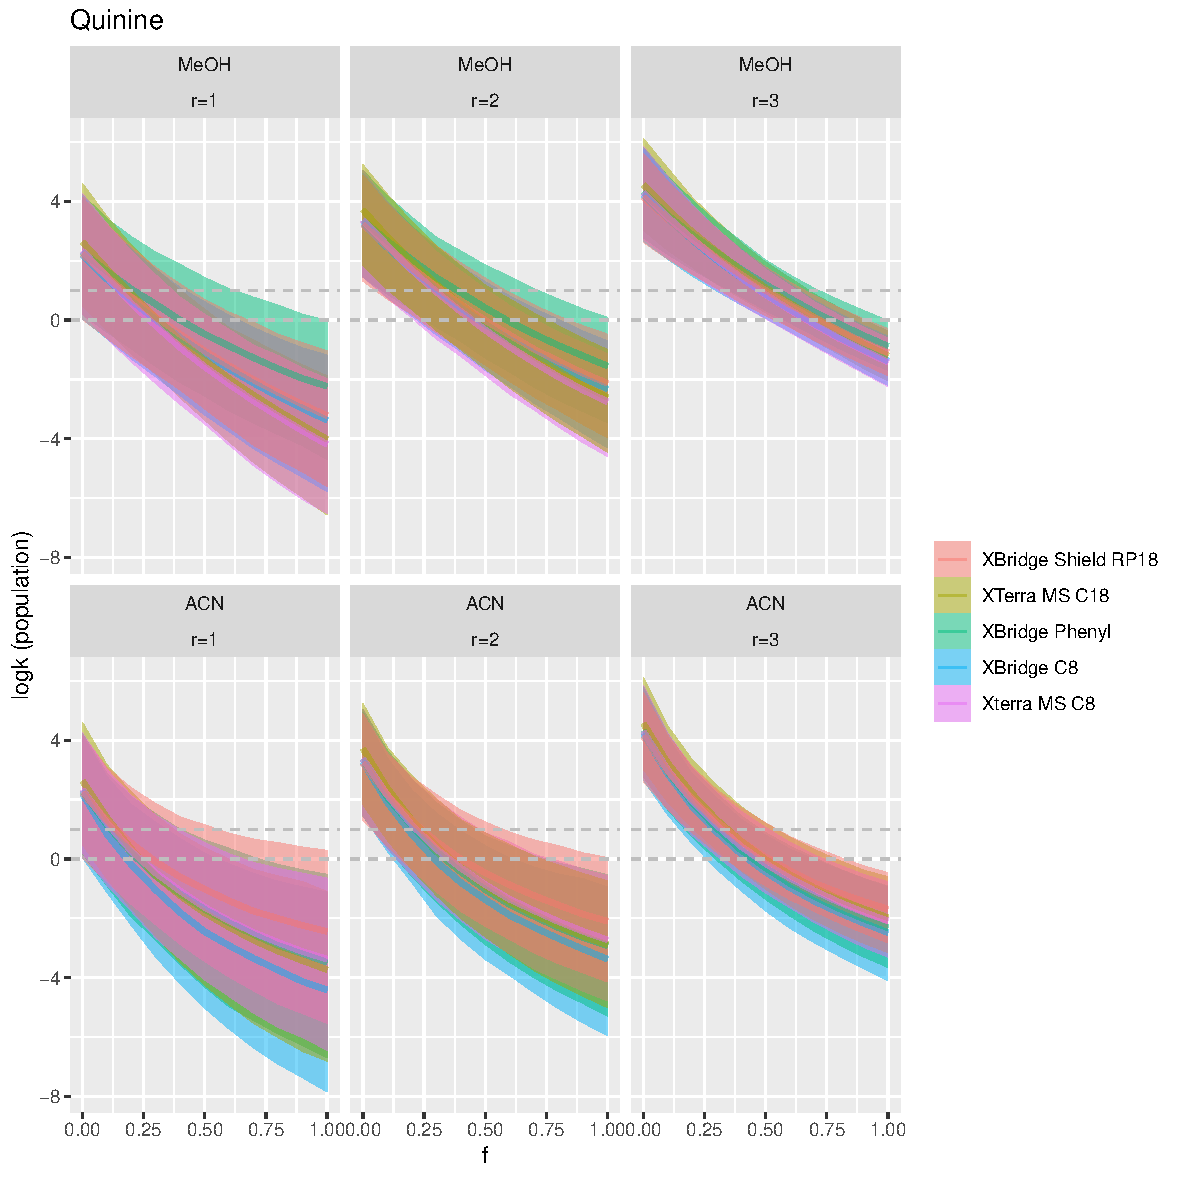
\includegraphics{../figures/izoparam/isopred/Quinine.population.pdf}

\newpage{}

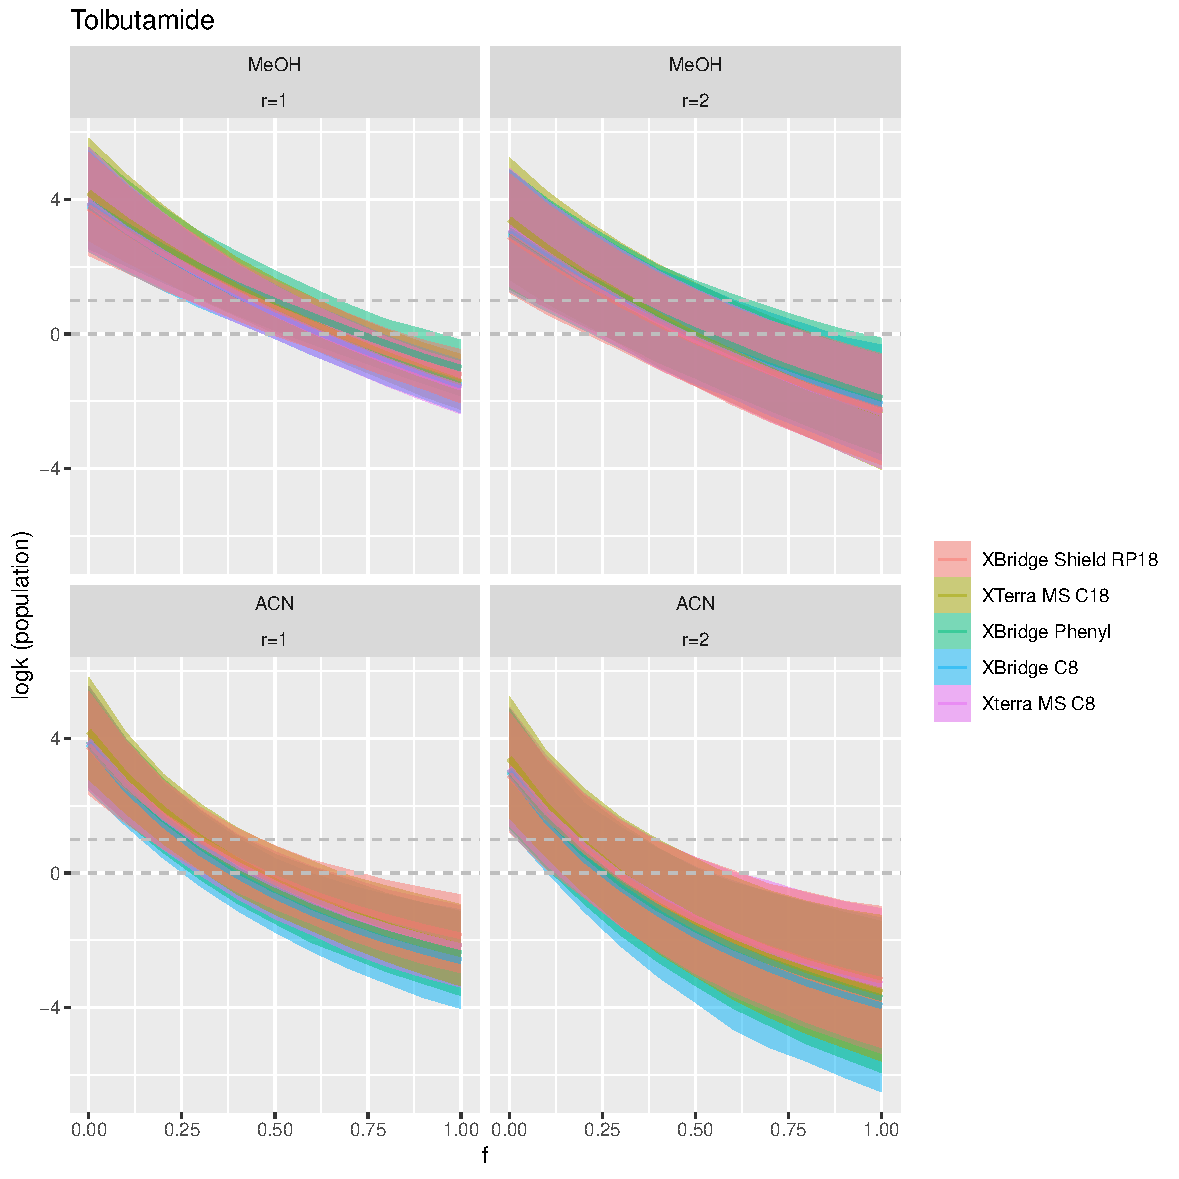
\includegraphics{../figures/izoparam/isopred/Tolbutamide.population.pdf}

\newpage{}

\hypertarget{figure-s10.-the-expected-utility-maps-based-on-individual-predictions.}{%
\section{Figure S10. The expected utility maps based on individual
predictions.}\label{figure-s10.-the-expected-utility-maps-based-on-individual-predictions.}}

The expected utility map for each column:

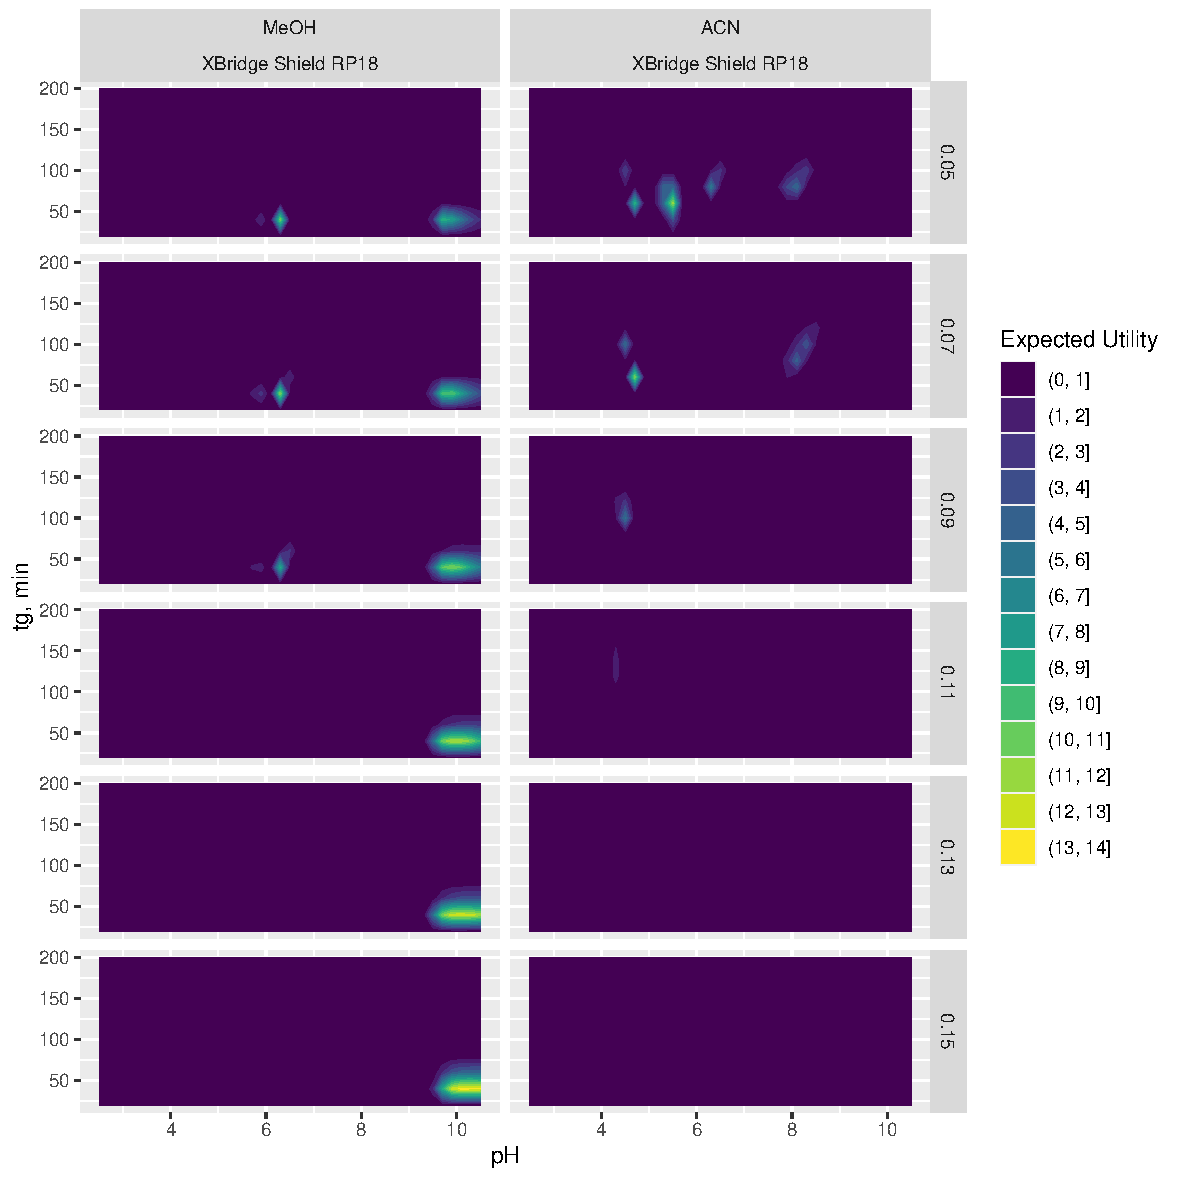
\includegraphics{../figures/casestudy1/utilitymap/utilitymap1.pdf}

\newpage{}

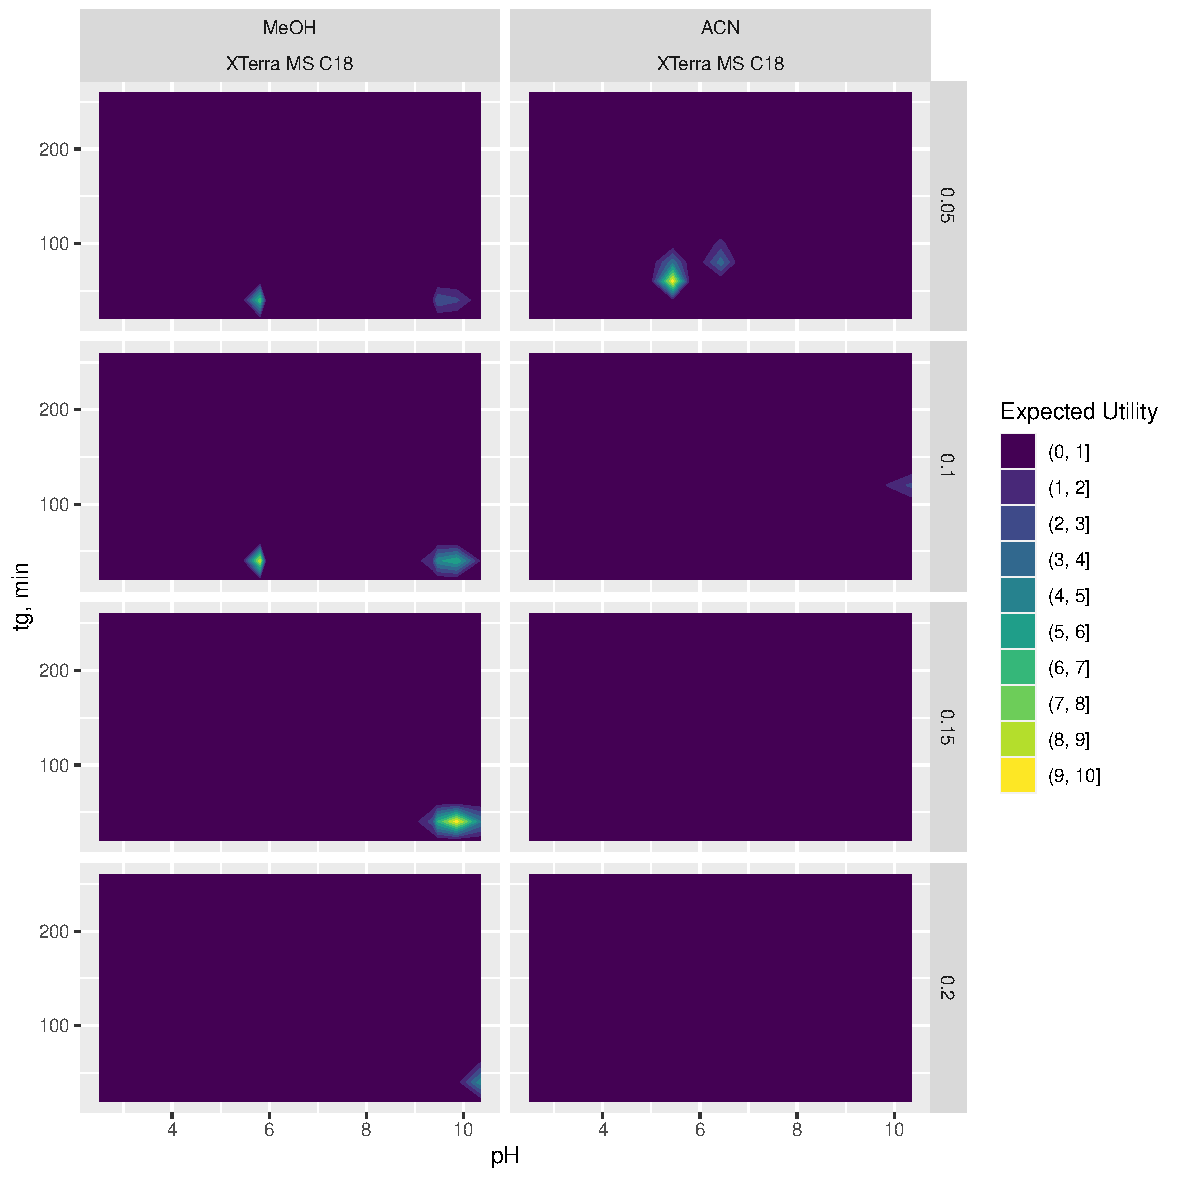
\includegraphics{../figures/casestudy1/utilitymap/utilitymap2.pdf}

\newpage{}

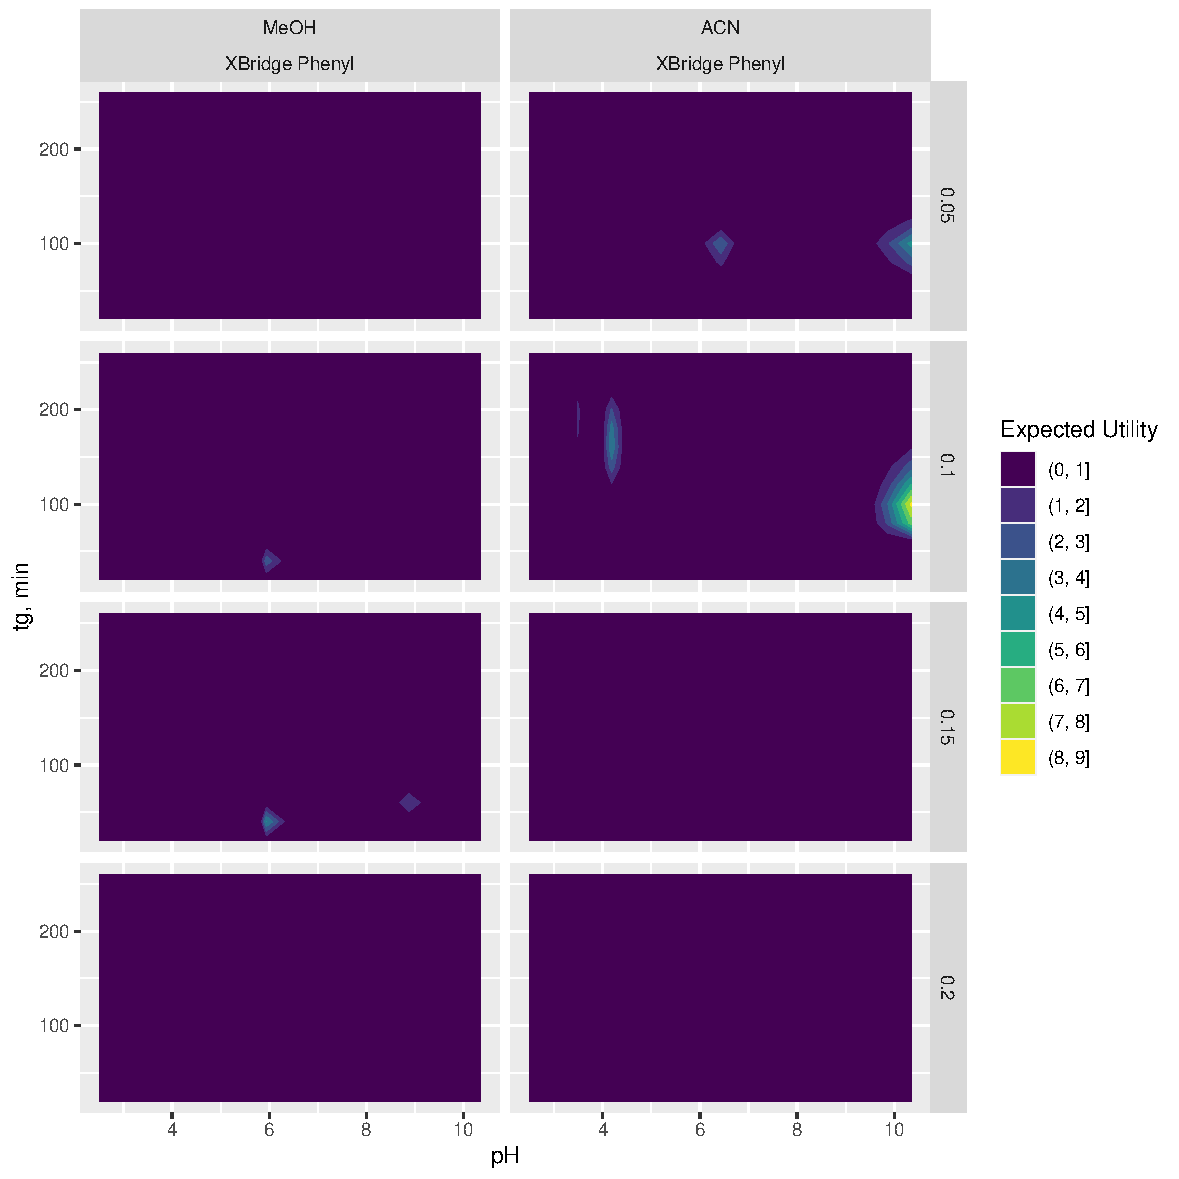
\includegraphics{../figures/casestudy1/utilitymap/utilitymap3.pdf}

\newpage{}

\includegraphics{../figures/casestudy1/utilitymap/utilitymap4.pdf}

\newpage{}

\includegraphics{../figures/casestudy1/utilitymap/utilitymap5.pdf}

\newpage{}

\hypertarget{figure-s11.-the-expected-utility-maps-based-on-limited-data-predictions.}{%
\section{Figure S11. The expected utility maps based on limited data
predictions.}\label{figure-s11.-the-expected-utility-maps-based-on-limited-data-predictions.}}

The expected utility map for each column:

\includegraphics{../figures/casestudy2/utilitymap/utilitymap1.pdf}

\newpage{}

\includegraphics{../figures/casestudy2/utilitymap/utilitymap2.pdf}

\includegraphics{../figures/casestudy2/utilitymap/utilitymap3.pdf}

\newpage{}

\includegraphics{../figures/casestudy2/utilitymap/utilitymap4.pdf}

\newpage{}

\includegraphics{../figures/casestudy2/utilitymap/utilitymap5.pdf}

\newpage{}

\hypertarget{licenses}{%
\section*{Licenses}\label{licenses}}
\addcontentsline{toc}{section}{Licenses}

\begin{itemize}
\tightlist
\item
  Code \& copy; 2023, Paweł Wiczling, licensed under BSD-3.
\item
  Text \& copy; 2023, Paweł Wiczling, licensed under CC-BY-NC 4.0.
\end{itemize}

\hypertarget{original-computing-environment}{%
\section*{Original Computing
Environment}\label{original-computing-environment}}
\addcontentsline{toc}{section}{Original Computing Environment}

\begin{verbatim}
R version 4.1.3 (2022-03-10)
Platform: x86_64-w64-mingw32/x64 (64-bit)
Running under: Windows 10 x64 (build 22621)

Matrix products: default

locale:
[1] LC_COLLATE=Polish_Poland.1250  LC_CTYPE=Polish_Poland.1250   
[3] LC_MONETARY=Polish_Poland.1250 LC_NUMERIC=C                  
[5] LC_TIME=Polish_Poland.1250    

attached base packages:
[1] stats     graphics  grDevices utils     datasets  methods   base     

other attached packages:
[1] cmdstanr_0.5.3   kableExtra_1.3.4 dplyr_1.1.3     

loaded via a namespace (and not attached):
 [1] tidyselect_1.2.0     xfun_0.32            colorspace_2.0-3    
 [4] vctrs_0.6.2          generics_0.1.3       htmltools_0.5.3     
 [7] viridisLite_0.4.1    yaml_2.3.7           utf8_1.2.3          
[10] rlang_1.1.0          pillar_1.9.0         glue_1.6.2          
[13] withr_2.5.0          distributional_0.3.1 matrixStats_0.62.0  
[16] lifecycle_1.0.3      stringr_1.5.0        posterior_1.3.1     
[19] munsell_0.5.0        gtable_0.3.1         ragg_1.2.5          
[22] rvest_1.0.3          codetools_0.2-18     evaluate_0.16       
[25] knitr_1.40           fastmap_1.1.0        fansi_1.0.4         
[28] scales_1.2.1         backports_1.4.1      checkmate_2.2.0     
[31] webshot_0.5.4        jsonlite_1.8.7       abind_1.4-5         
[34] farver_2.1.1         systemfonts_1.0.4    textshaping_0.3.6   
[37] tensorA_0.36.2       ggplot2_3.4.2        digest_0.6.29       
[40] stringi_1.7.8        grid_4.1.3           cli_3.6.1           
[43] tools_4.1.3          magrittr_2.0.3       tibble_3.2.1        
[46] pkgconfig_2.0.3      data.table_1.14.8    xml2_1.3.3          
[49] rmarkdown_2.16       svglite_2.1.1        httr_1.4.5          
[52] rstudioapi_0.14      R6_2.5.1             compiler_4.1.3      
\end{verbatim}



\end{document}
